% !TeX TS-program = latex
\RequirePackage{fix-cm}
%Journal of Mathematical Imaging and Vision
\documentclass[twocolumn]{svjour3}

\pdfoptionpdfminorversion=7

\smartqed  % flush right qed marks, e.g. at end of proof

\usepackage{times}
\usepackage{bm,bbm}
\usepackage{amsmath,amssymb}
\usepackage{graphicx,subfigure}
\usepackage{url}
\usepackage{units}
\usepackage{cite,balance}
\usepackage{comment}
\usepackage{multirow}
\usepackage{booktabs}
\usepackage{microtype}
\usepackage{siunitx}
\usepackage{color}
\usepackage{float}
%\usepackage{auto-pst-pdf}

\usepackage{mathptmx}

\usepackage{array}
\usepackage{varwidth}


\usepackage[normalem]{ulem} %%%% para tachar texto

%-----------------------
%Bibliography style
%\usepackage[numbers]{natbib}

%\newtheorem{definition}{Definition}
%\newtheorem{proposition}{Proposition}
\newcommand{\at}[2][]{#1|_{#2}}
%\newcommand{\K}{\text{K}}

\newcommand{\mc}[1]{\multicolumn{1}{c}{#1}}
\newcommand{\argmin}{\operatorname*{\text{arg min }}}

\ifpdf
\graphicspath{{/Users/acfrery/Documents/Alunos/Julia Cassetti/Figures/PaperTesis}{/Users/acfrery/Documents/Alunos/Julia Cassetti/Figures/PaperTesis/ConModificacionAlejandro}{/Users/acfrery/Documents/Alunos/Julia Cassetti/Figures/PaperTesis/Viejos}}
\else
\graphicspath{{/Users/acfrery/Documents/Alunos/Julia Cassetti/Figures/PaperTesis}{/Users/acfrery/Documents/Alunos/Julia Cassetti/Figures/PaperTesis/ConModificacionAlejandro}{/Users/acfrery/Documents/Alunos/Julia Cassetti/Figures/PaperTesis/Viejos}}
\fi

\begin{document}

\title{An Improved Minimum-Distance Texture Estimator for Speckled Data under the $\mathcal{G}^0$ Model
\thanks{This work was partially supported by CNPq and Fapeal.}
}
%\subtitle{Do you have a subtitle?\\ If so, write it here}

%\titlerunning{Short form of title}        % if too long for running head

\author{Julia~Cassetti         \and
Alejandro~C.~Frery %etc.
}

%\authorrunning{Short form of author list} % if too long for running head

\institute{Julia Cassetti \at
Instituto de Desarrollo Humano, Universidad Nacional de General Sarmiento, Pcia. de Buenos Aires, Argentina. \\
Tel.: (54 11) 4469-7701/7702/7703\\
Fax: Fax: (54 11) 4469-7734\\
\email{julia.cassetti@gmail.com}           %  \\
%             \emph{Present address:} of F. Author  %  if needed
\and
Alejandro C.\ Frery\at
School of Mathematics and Statistics, Victoria University of Wellington\\
PO Box 600, Wellington 6140 New Zealand\\
\email{alejandro.frery@vuw.ac.nz}
}

\date{Received: 29 May 2020 / Accepted: date}
% The correct dates will be entered by the editor

\maketitle

\begin{abstract}
The $\mathcal G^0$ distribution is an apt model for speckled data, such as SAR imagery, because it possesses the ability to characterize areas with different degrees of texture. 
In the monopolarized case, this distribution depends on three parameters: the texture, the scale, and the number of looks. 
The first one is related to the roughness of the image, so its estimation deserves special attention.
This paper proposes and compares estimation methods of the texture parameter in intensity format. 
We treat the multilook case. The proposal is to estimate this parameter by minimizing the triangular distance between the $\mathcal G^0$ density and an estimate of the underlying density function using asymmetric kernels.    
We assess the properties of these estimators with analytic results and simulation. 
We use actual images to evaluate the performance of our proposal.
\keywords{Synthetic aperture radar\and parameter estimation\and kernel estimation\and minimum distance estimator\and texture analysis.}
% \PACS{PACS code1 \and PACS code2 \and more}
% \subclass{MSC code1 \and MSC code2 \and more}
\end{abstract}

\section{Introduction}
\label{intro}

Remote sensing with Synthetic Aperture Radar (SAR) data has become a vital tool for environmental studies because it produces high-resolution images of targets and landscapes. 
It has several advantages over optical and infrared systems due to its ability to acquire images independently of the sunlight and weather conditions. 
For this reason, these images have a wide range of practical applications: environmental monitoring~\cite{White1991,Brisco2013}, and
earthquake study to map the surface deformation~\cite{Yinghui2017}, among others.  
%quality-assessment methods of multisensor SAR data fusion is investigated in~\cite{Abdikan2014}. 
Nevertheless, SAR images have the disadvantage of having speckle noise, which appears from the use of coherent illumination~\cite{SARImageStatisticalModelingPartISinglePixelStatisticalModels}. 
This kind of noise is a characteristic of technologies that
employ coherent illumination, such as microwaves, sonar, laser, and ultrasound. 
Speckle noise makes the analysis and interpretation of this kind of image a challenging task.
%But SAR images have the disadvantage of having speckle noise, which makes the analysis and interpretation of these kinds of images a challenging task.

The multiplicative model has been successfully used in modeling SAR images.
It describes the observed data as the product of two statistically independent random variables representing the target information and the speckle noise respectively. 
In this context, the $\mathcal{G}^0$ model has proved to describe textured and extremely textured areas better than other models~\cite{Frery97,MejailJacoboFreryBustos:IJRS}. 
Three parameters index this model: 
one directly associated with the texture, 
other being a scale parameter, 
and the third related to the signal-to-noise ratio.

The texture is of paramount importance, as it describes the target roughness locally.
In particular, it can be related to the number of elementary backscatterers~\cite{AGeneralizedGaussianCoherentScattererModelforCorrelatedSARTexture} and, as such, its estimation is essential.

Several works have studied parameter estimation under the $\mathcal{G}^0$ model. 
Among the estimation techniques available, moments (or analogy) and maximum likelihood estimators are among the most popular. 
%Bian~\cite{Bian2013} proposes a method based on fractional lower-order statistics to estimate a polarimetric SAR covariance matrix in an alpha-stable distribution.
Refs.~\cite{VasconcellosFrerySilva:CompStat,CribariFrerySilva:CSDA} describe attempts to improve the performance of these estimators concerning bias and mean squared error using either resampling or analytic procedures. More recently, using a connection between the Mellin's transform, several estimators based on logcumulants and logmoments have been proposed in~\cite{MellinAnalysisPolSAR,BujorTrouveValetNicolas2004,khan2014}. 

Bustos et al.~\cite{BustosFreryLucini:Mestimators:2001} and
Allende et al.~\cite{AllendeFreryetal:JSCS:05} studied the performance of maximum likelihood estimators under the $\mathcal{G}^{0}$ model for amplitude data, showing that they critically lose robustness for moderated outliers in extremely textured areas, whereas in textureless areas this occurs for severe outliers.
As expected, the lack of robustness is more pronounced for small samples. 
They proposed M and AM estimators for the texture with good performance under contamination, but they suffer from numerical problems, especially with small samples.

Tison et al.~\cite{Tison2004} showed that estimators based on logcumulants 
are well-suited to model amplitude single-look data from urban areas, where very large values are frequently observed.
Nevertheless, that work overlooks the fact that estimation under the $\mathcal G^0$ distribution is more sensitive to very small values rather than to extremely large ones.
In this work, we explore this fact and propose suitable solutions using kernels.

A good estimator should have good behavior if the data come from the assumed model, and it should not present large deviations against small perturbation from the assumed model.
In this sense, Refs.~\cite{APSAR2013ParameterEstimationStochasticDistances,gambini2015} are recent attempts at obtaining robust estimators for the textured parameter of the $\mathcal{G}^0$ model for intensity data.

In general, the approach is to find the parameters that minimize dissimilarity measures ($d$) between the actual density function $f_{\theta}$, which depends on the $\theta$ parameter, and an estimation of the underlying density function $\widehat{f}$. 
These are the minimum distance estimators (MDE), defined as:
\begin{align}
\label{MDEGeneral}
\widehat{\theta}=
\argmin_{\theta\in\Omega}
%\mathop{\rm argmin} \limits_{\theta\in\Omega} 
d(f_{\theta}, \widehat{f}),
\end{align}
where $\theta\in\Omega$ is the parameter to be estimated,
and $\Omega$ is the parameter space. 
In this oncoming, two elements are needed: a measure of distance and $\widehat{f}$.

Wolfowitz~\cite{wolfowitz1953, wolfowitz1957} studied this class of estimators and showed that, under general conditions, they are strongly consistent. 
Beran~\cite{Beran1977} proposed an MDE estimator using Hellinger's distance between a theoretical model and a nonparametric density estimator using symmetric kernels. 
The work showed that this estimator is asymptotically efficient for certain parametric families of densities. 
Parr and Schucany~\cite{parr1982} show that, under certain conditions, the MDE estimator between the empirical distribution function and theoretical distribution function is strongly consistent. 
Cao et al.~\cite{cao1995minimum} proposed to minimize a distance between the theoretical density function and $\widehat{f}$ using the classic symmetric kernel estimator to estimate $f$. 
They showed, under specific considerations, the strong consistency of these estimators, and studied its asymptotic normality for the $L^2$ metric.

Refs.~\cite{Parzen62,Roseanblatt56} presented nonparametric kernel estimators using symmetric kernels, but when the function to be estimated has bounded support, this kind of estimators may assign probability mass outside the support~\cite{Silverman1986}, leading to biased estimations in a neighborhood of the boundary.
Some authors aim to use asymmetric kernel estimators to solve this problem. 
Chen~\cite{chen1999,chensx2000} presented Beta and Gamma ($\Gamma$) kernels.
Scaillet~\cite{Scaillet2004} introduced the inverse Gaussian (IG) and reciprocal inverse Gaussian (RIG) kernels.
Bouezmarni and Scaillet~\cite{bouezmarni2005} proved the consistency under the $\Gamma$, IG and RIG kernels. 
Jin and Kawczak~\cite{Jin2003} proposed the Birnbaum-Saunders (BS) and Lognormal (LN) kernels. 
Ref.~\cite{libengue2013} also treats these kernels. 
These estimators vary their shape according to the observation. This feature allows obtaining different degrees of smoothing~\cite{Scaillet2004}, and, as they do not assign weight outside the density function support, they are free of boundary bias~\cite{chensx2000}.

In the last decade, concepts related to information theory have gained interest in image processing. 
In particular, several measures have been proposed to reflect the closeness among the models that describe samples. 
Especially the concept of stochastic divergence has found applications in areas as diverse as signal and image processing~\cite{Aviyente2007}, automatic region detection in SAR imagery~\cite{SilvaCribariFrery:ImprovedLikelihood:Environmetrics,Nascimento2009}, 
speckle filters~\cite{Penna2019}, as contrast measures. 
Unsupervised classification strategies were applied to Polarimetric Synthetic Aperture Radar (PolSAR) images in~\cite{Carvalho2019}.

Cassetti et al.~\cite{APSAR2013ParameterEstimationStochasticDistances} proposed an MDE estimator for the texture parameter of the $\mathcal{G}^0$ model and assessed different stochastic distance with a nonparametric estimation of the underlying density function using histograms. 
Gambini et al.~\cite{gambini2015} proposed to estimate $f$ using the IG asymmetric kernel with a bandwidth chosen empirically; 
they found the estimator by minimizing Eq.~\eqref{MDEGeneral} by inspecting a grid of values of $\alpha$. 
The authors concluded that the triangular distance is the best suited for this problem, and showed that their proposal outperforms the Logcumulant estimator in terms of mean squared error, bias, convergence, and robustness. 
So, the results were promising, with venues for improvement which are explored in this work.

In this paper, we improve the Gambini et al.~\cite{gambini2015} proposal. 
We use $\Gamma$ and LN kernels instead of the IG kernel, showing that the latter presents a larger integrated mean square error and a higher percentage of non-convergence cases than the others.
Regarding bandwidth choice, we use Least Squared Cross-Validation (LSCV)~\cite{Rudemo1982} for bandwidth selection in place of the empirical selection. 
Furthermore, we use a search algorithm to find the minimum of the MDE estimator instead of a loop through a grid of $\alpha$ values. 

We compare the performance of the proposed estimator for the texture parameter of the $\mathcal{G}^0$ model for intensity data with Maximum Likelihood (ML) and Logcumulants (LC) methods in terms of convergence, bias and mean squared error and sensitivity to contamination. 
We obtain excellent results, especially for small sample sizes.

The rest of the paper unfolds as follows: 
Section~\ref{sec_SAR} recalls the main features of the $\mathcal{G}^0$ model for intensity data.
%Section~\ref{pareto} shows the relationship between this model and the Pareto distribution and proposes a new estimator for the single-look case.
Section~\ref{distancekernel} presents the discussion of estimation with stochastic distances and asymmetric kernels. 
Section~\ref{simulation} presents the main results of the Monte Carlo study. Section~\ref{application} shows an application of our proposal to actual SAR images.
Section~\ref{conclusion} concludes the article discussing promising directions for future research.

\section{The $\mathcal{G}^0$ Model}
\label{sec_SAR}

The return in monopolarized SAR images can be modeled as the product of two independent random variables, one corresponding to the backscatter $X$, and other to the speckle noise $Y$. 
In this manner, $Z=X Y  $ represents the return $Z$ in each pixel under the multiplicative model.

The speckle noise in intensity format $Y$ is modeled as a $\Gamma$ distributed random variable with unitary mean and shape parameter $L\geq1$, the number of looks, while the backscatter $X$ is considered to obey a Reciprocal of Gamma law. 
These assumptions give rise to the $\mathcal{G}^{0}$ distribution for the return $Z$.
Given the mathematical tractability and expressive power of the $\mathcal{G}^{0}$ model~\cite{MejailJacoboFreryBustos:IJRS,mejailfreryjacobobustos2001} it represents an attractive choice for SAR data modeling.

The density function for intensity data is given by
\begin{equation}
f_{\mathcal{G}^{0}(z)} =\frac{L^{L}\Gamma ( L-\alpha
	) }{\gamma ^{\alpha }\Gamma ( -\alpha ) \Gamma (
	L) }\cdot  
\frac{z^{L-1}}{( \gamma +zL) ^{L-\alpha }},%
\label{ec_dens_gI0}
\end{equation}
where $-\alpha,\gamma ,z>0$ and $L\geq 1$. 
The $r$-order moments are
\begin{equation}
\text{E}(Z^r) =\Big(\frac{\gamma}{L}\Big)^r\frac{\Gamma ( -\alpha-r )}{ \Gamma (-\alpha) }
\frac{\Gamma (L+r )}{\Gamma (L)},
\label{moments_gI0}
\end{equation}
provided $\alpha<-r$, and infinite otherwise.

Mejail et al.~\cite{MejailJacoboFreryBustos:IJRS} proved a relationship between $\mathcal G^0$ distributions and the Fisher-Snedekor $F$ law.
With this result, using standard functions available in most computational statistics environment as, for instance, the \texttt R programming language and environment~\cite{RLanguage}, the cumulative distribution function of a $\mathcal G^0(\alpha,\gamma,L)$ distributed random variable $F_{\alpha,\gamma,L}$ can be obtained as
\begin{equation}
F_{\alpha,\gamma,L}(z) = \Upsilon_{2L, -2\alpha}(-\alpha  z / \gamma),
\label{eq:CDFG0}
\end{equation}
for every $z>0$, where $\Upsilon_{2L, -2\alpha}$ is the cumulative distribution function of a Fisher-Snedekor random variable with $2L$ and $-2\alpha$ degrees of freedom.
This relationship is useful for obtaining the quantiles and entropy, among other features of this distribution.

It is essential to achieve accurate and robust estimates of $\alpha$ because it is related to the target's texture. 
Values close to zero ($\alpha \in (-3,-1)$) suggest extreme texture, as in urban areas. 
As the value decreases, the texture is also reduced going, usually, from $\alpha \in (-6,-3]$ in forest zones up to $\alpha\in(-\infty,-6)$ in textureless targets, e.g., pasture or crops. So, its estimation deserves special attention.

Maximum likelihood estimation is the classical approach for parametric estimation of a density function because it has optimal asymptotic properties in terms of bias and variance, and well-known asymptotic distributional properties.
To reduce our discussion to a single parameter, we based the forthcoming analysis on the condition of unitary mean, i.e., $E(Z)=1$, which links the texture and the brightness parameters:
\begin{align}
\label{RelationAlphaGamma}
\gamma^* =-\alpha-1.
\end{align}

Let $Z_1,\dots, Z_n$ be an independent random sample of finite size $n$ from the $\mathcal G^0(\alpha,\gamma^*,L)$ distribution.
A maximum likelihood estimator of $\alpha$ for $L$ known, denoted $\widehat\alpha_{\text{{ML}}}$, is any value in $(-\infty,-1)$ that maximizes the loglikelihood function:
\begin{align}
\hat{\alpha}_{\text{{ML}}}=&\argmin_{\alpha \in (-\infty,-1)}\log \Gamma(L-\alpha)-
\alpha\log(-1-\alpha)-\log\Gamma(-\alpha) \nonumber \\
&\mbox{}+\frac{\alpha-L}{n} \sum_{i=1}^n\log(-1-\alpha+L Z_i).
\label{ML}
\end{align}
Notice that we are interested in finite sample size cases, for which we do not have to take into account the possibility of infinite distributional variance.
We limit the search space to cases with finite distributional mean by avoiding the region $[-1,0)$.

%We employed the Broyden-Fletcher-Goldfarb-Shanno (BFGS) method~\cite{Luenberger2008}, which does not require the derivative of~\eqref{ML}.
We employed the L-BFGS-B version of the Broyden-Fletcher-Goldfarb-Shanno (BFGS) method~\cite{Luenberger2008} to find the optimum of this function taking as a starting point $\alpha_0$ the alpha moment estimator when it exists. Otherwise we consider $\alpha_0=-1.5$. This algorithm is a quasi-Newton type optimization method that allows box constraints and is widely used in Computer Graphics and Scientific Computing~\cite{FEI2014}. 
These methods do not need the Hessian matrix but use an approximation that is updated in each iteration and, thus, they only require the function and its gradient. 

Function~\eqref{ML} is, in general, unimodal, but, depending on the sample, it may be monotonically decreasing or flat~\cite{FreryCribariSouza:JASP:04}. 
This behavior is responsible for the failure of algorithms to converge to a global maximum.


\section{Minimum distance estimator and asymmetric kernels}
\label{distancekernel}

The Minimum Distance Estimator (MDE) approach is a nonparametric methodology that proposes estimators by finding the value of the parameters that make the theoretical model as close as possible to the information provided by the sample. 
There are two elements involved: one is the measure of distance that allows quantifying proximity, and the other is the information that comes from the sample.

Regarding the sample information, some measures link the empirical distribution function and the theoretical model, and others measure the discrepancy between a nonparametric estimate of the underlying density function and the actual density. 
In general, the distribution function is absolutely continuous, so it may be convenient to consider MDE estimators in terms of the density function. 

Information theory provides divergence measures to discriminate between density functions in a statistical sense. 
Salicr\'u et al.~\cite{Salicru1994} proposed a family of such measures, called $(h,\phi)$-divergences, that includes the Kullback-Leibler divergence,  
the $\phi$-divergences presented by Csisz\'ar~\cite{Csiszar1967}, 
and the generalizations of the $J$- and $R$-divergences defined by Taneja ~\cite{Taneja1989}, among others.
These $(h,\phi)$-divergences can be easily turned into distances, and into statistical tests.

Cassetti et al.~\cite{APSAR2013ParameterEstimationStochasticDistances} used the notion of minimizing a stochastic distance to propose a new estimator for the $\alpha$ parameter in the $\mathcal{G}^0$ model. 
This estimator is defined as
\begin{equation}
\widehat{\alpha}_n=\argmin_{\alpha\in\Omega} d(f_{\mathcal{G}^0}, \widehat{f}_n),
\label{MDE}
\end{equation}
where $\Omega$ is the parameter space, $d$ is a dissimilarity measure or stochastic distance between the theoretical density function $f_{\mathcal{G}^0}$ and a nonparametric estimator $\widehat{f}_n$ of the underlying density function.
The authors used histograms to compute $\widehat{f}_n$, and assessed the Hellinger, Bhattacharyya, R\'enyi, and Triangular distances. 
They chose the Triangular distance because it presented the best performance.

The Triangular distance is defined as:
\begin{equation}
d_{\text{{T}}}(f_{\text{{V}}},f_{\text{{W}}})=\int_{S}\frac{\big(f_{\text{{V}}}(x)-f_{\text{{W}}}(x)\big)^2}{f_{\text{{V}}}(x)+f_{\text{{W}}}(x)}dx,
\label{DT}
\end{equation}
where $f_{\text{{V}}}$ and $f_{\text{{W}}}$ are two density functions with common support $S$.

Gambini et al.~\cite{gambini2015} estimated the underlying density function with asymmetric kernels.
In particular, the authors used the IG kernel, defined in subsection~\ref{asymmetrickernel}. 
In this work, we use $\Gamma$ and LN kernels because they outperform the IG kernel: they have less integrated mean quadratic error and fewer cases of non-convergence than the IG kernel.
%It is noteworthy that $\Gamma$ model kernels that are presented in this work.

\subsection{Gamma, Lognormal and Inverse Gaussian Kernels}
\label{asymmetrickernel}

Classical density estimation with kernels usually uses symmetric kernels. 
However, when the density has bounded support, such estimators present boundary bias. 
This bias appears because the symmetric kernels assign weight outside the support when the estimation takes place near the boundary.

%	The asymmetric kernel estimator is an alternative to solve this problem. Several authors investigated such kernels: 
%	$\Gamma$ and Beta kernels were studied by Chen in~\cite{chensx2000} and in~\cite{chen1999}, respectively; 
%	Scaillet et al.~\cite{Scaillet2004} proposed the IG and the Reciprocal Inverse Gaussian (RIG) kernels; 
%	Jin et al~\cite{Jin2003} suggested Birnbaum-Saunders (BS) and LN kernels, among others. 
%	Convergence properties were studied in~\cite{bouezmarni2005,libengue2013}. In this section, we present the asymmetric kernels used in this work.

Let $ Z = Z_1,\dots, Z_n$ be a random sample of size $n$, from an unknown density probability function $f$ with positive support, an estimate of the underlying density function is:
$$
\widehat{f}_b(z)=\frac{1}{n}\sum_{i=1}^n K_{\theta(z,b)}(Z_i),
$$ 
where $K$ is the asymmetric kernel, $b$ is the bandwidth and ${\theta}(z,b)$ is the parameter vector.

Among the many available asymmetric kernels, we used the $\Gamma$ and LN kernels defined, for every $t>0$, as:
\begin{align}
K_{{\Gamma}_{{\theta}(z,b)}}(t) & =\frac{1}{\Gamma(\frac{z}{b}+1)b^{\frac{z}{b}+1}} t^{-{z}/{b}} \exp\{-{t}/{b}\},
\label{gammakernel}\\
K_{{\text{{LN}}}_{{\theta}(z,b)}}(t) & =\frac{1}{t \sqrt{2 \pi} b} \exp\Big\{-\frac{\left(\log t - \log z -b^2\right)^2}{2b^2}\Big\},
\label{LNkernel}
\end{align}
respectively for $t,z,b>0$.

As mentioned in Section~\ref{distancekernel}, Gambini et al.~\cite{gambini2015} used the Inverse Gaussian kernel defined as
\begin{align}
K_{\text{IG}}( t; z_i,b) & =\frac{1}{\sqrt{2\pi b t^3}} 
\exp\Big\{-\frac{1}{2b z_i} \Big(\frac{t}{z_i}+\frac{z_i}{t}-2\Big)\Big\}.
\end{align}

The rationale for using these kernels is the following:
the $\mathcal{G}^0$ model embeds the $\Gamma^{-1}$ distribution;
the $\mathcal{G}^H$ model (also used for describing SAR data; cf.~\cite{PolarimetricSegmentationBSplinesMSSP}) considers the IG distribution to model the backscatter;
the Lognormal distribution is a widely used empirical model to describe SAR data~\cite{Gao2010}. 

The bandwidth is a sensitive choice in nonparametric density estimation. 
Gambini et al.~\cite{gambini2015} chose, empirically, $b=n^{-1/2}/5$. 
In this work, we propose the Least Square Cross-Validation~\cite{Wu1997} (LSCV) method to find an appropriate value.

Figure~\ref{EstimacionLNyGAyIG} shows an estimation example of the $\mathcal{G}^0$ model. 
We generated a sample from a $\mathcal{G}^0$ distribution of size $n=25$, $L = 8$, $\alpha=-5$ and $\gamma=4$. 
The solid black line is the actual density function. 
These kernels fit reasonably well the theoretical density function, even for a small sample size. 
The IG kernel presents a good approximation to the true density function at the center of the function, although with heavier tails. 
The $\Gamma$ and LN kernels show a better fit, the latter with higher kurtosis than the other kernels.

\begin{figure}[hbt]
\centering
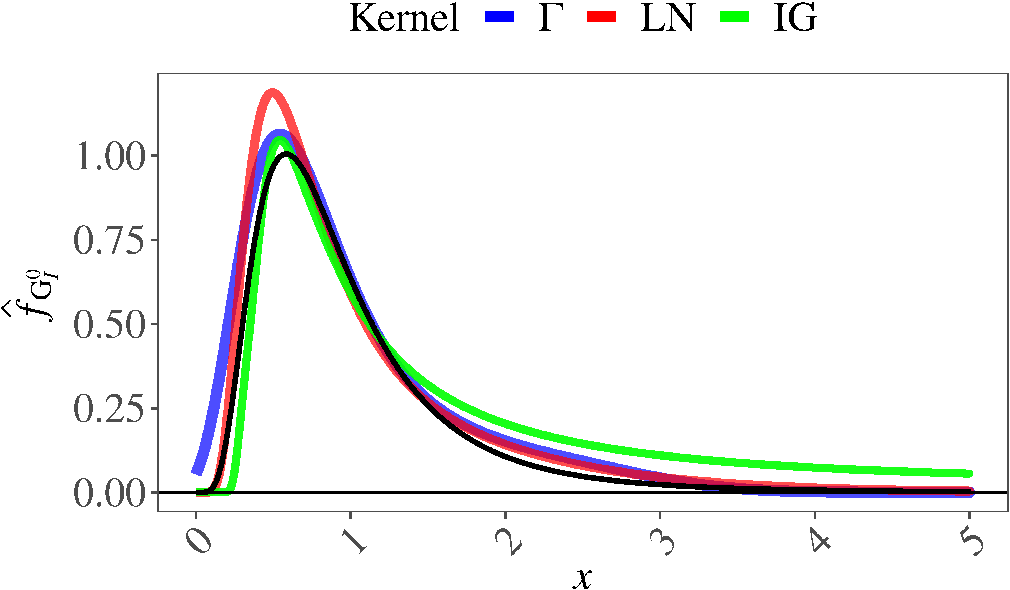
\includegraphics[width=\linewidth]{NucleosGALNyIG}
\caption{$\widehat{f}_{\mathcal{G}^0}$ for $L=8$, $\alpha=-5$, $\gamma=4$ and $n=25$ using $\Gamma$, LN, and IG kernels, and LSCV for bandwidth selection.}\label{EstimacionLNyGAyIG}
\end{figure}
%JC Programa: GraficoEstimacionDensidadConNucleos.R

It is essential to have measures that quantify the quality of the estimation. 
We used the Integrated Mean Square Error (MISE) because it measures the average behavior of the estimator on different samples. 
It is defined as
\begin{align}
\label{Mise}
\text{MISE}(\widehat{f}_b(Z_1,\ldots,Z_n))=&E\left[\int_\mathbb{R} \big(\widehat{f}_b(z,Z_1,\ldots,Z_n)-f(z)\big)^2 \right].
\end{align}

It is important to note that these kernel estimators are free of boundary bias and achieve the convergence rate $n^{-4/5}$ for the MISE.
The scale parameter is set such that the expected value of the return $Z$ is one. 
This condition leads to the following relation $\gamma_0^*=-\alpha-1$.

\subsection{Logcumulant estimator}\label{lc}

%%% ACF This paragraph is not clear
The relationship between the moments of a random variable and its characteristic function, related to the Fourier transform of the probability density function, is well-known. 
When the moments of order $k$ exist, they can be calculated through the derivatives of order $k$ of the characteristic function.

In the same sense, Nicolas et al.~\cite{nicolas2002} defined the first characteristic function of the second kind as the Mellin transform of its density when it has positive support. 

Gambini et al.~\cite{gambini2015} show that the LC estimator for the $\alpha$ parameter of the $\mathcal{G}^0$ distribution, under the relationship~\eqref{RelationAlphaGamma}, is the solution of 
\begin{equation} \label{eq:logm}
\frac{1}{n} \sum_{i=1}^n\log z_i =   -\log \frac{L}{-\widehat\alpha_{\text{{LC}}}-1} + \Psi^0(L) - \Psi^0(-\widehat\alpha_{\text{{LC}}}).
\end{equation}
The right term of the equation~\eqref{eq:logm} is a monotone decreasing function of $\alpha$. Therefore, this equation has a single root or none. 
This estimator is widely used in SAR image processing. 
Refs~\cite{MellinAnalysisPolSAR,BujorTrouveValetNicolas2004,khan2014} applied this methodology due to its nice properties and good performance. 
More recently, Nogueira et al.~\cite{Nogueira2019} used the LC estimator applied in an unsupervised algorithm for SAR image segmentation.

We compare our proposal with LC and ML estimators because these a commonplace in the literature.

\subsection{Robustness analysis -- Stylized Samples}
\label{robustez}
Among the desirable properties of a good estimator, resistance to contamination is very important in practical applications. 
That is, it can produce reasonable estimations even when a proportion of the data does not come from the assumed model. 
This situation is of particular importance in the case of small sample sizes, e.g., when using filters defined on sliding windows of size $3 \times 3$, $5 \times 5$ or, for instance, $7 \times 7$. 
These windows may contain data from areas with different textures, for example, at the edges between different regions or corner reflectors (features that produce a few very large observations with respect to the background).

In image processing and analysis, it is difficult to grant the underlying hypothesis under which the techniques being employed hold, so the ability to perform well even under deviations from these assumptions is a requirement.

In order to assess the robustness of the proposed estimators, we consider different alternatives. 
The first one is to consider that, in a small proportion $\epsilon$, the data may suffer deviations of the theoretical model. 
In this case we define random variables $W \sim \mathcal{G}^0(\alpha_1,\gamma_1^*,L)$ and $U \sim \mathcal{G}^0(\alpha_2,\gamma_2^*,L)$, where $\gamma_1^*=-\alpha_1-1$ and  $\gamma_2^*=-\alpha_2-1$. 
We consider the Bernoulli random variable $B$ with a probability of success $\epsilon$ indicating the contamination ratio.   
We define $Z=BU+(1-B)W$ by its cumulative distribution function as
$
\epsilon {F}_{\alpha_2,\gamma_2^*,L}(z)+(1-\epsilon) {F}_{\alpha_1,\gamma_1^*,L}(z)
$.
This schema considers that, on average, a small proportion $\epsilon$ of the data come from the same family but with different parameters. 

%%% ACF Was this contamination model used in this work?
Sometimes a few pixels present an extremely high return value. 
This phenomenon is produced by a double bounce of the electromagnetic signal, or by a corner reflector, and is one of the sources of contamination in SAR imagery. 
Such outliers may provoke significant errors in the estimation, as we show in an application to a real image. 
The return in such can be modeled as $Z=BC+(1-B)W$, where $C$ is a large value, and $B$ and $W$ are defined as before.

A way of assessing how the estimator $T_n(z_1,\dots,z_n)$ behaves under contamination is by fixing $n-1$ observations and allowing one to vary.
This is the EIF -- Empirical Influence Function, but it depends on the particular sample.
To avoid this, Andrews et al.~\cite{Andrews1972}, proposed using the $i^{th}$ quantile of the assumed distribution as typical observations: $z_i=F^{-1}\big((i-1/3)/(n+1/3) \big)$, $1\leq i\leq n-1$.
This is the SEIF -- Stylized Empirical Influence Function that, among others, was used by Rousseeuw and Verboven~\cite{RousseeuwCSDA} for estimation with very small samples and by Allende et al.~\cite{AllendeFreryetal:JSCS:05} for AM estimators of the texture under the amplitude $\mathcal G^0$ law.

The quantiles of a $\mathcal G^0(\alpha,\gamma,L)$ random variable can be obtained by $\Upsilon^{-1}_{2L,-2\alpha}$, the inverse of~\eqref{eq:CDFG0}, also available in most statistical computing environments.


\section{Performance Analysis}\label{simulation}

This section presents empirical results about the quality of estimators for the texture parameter under the $\mathcal G^0$ distribution. 
We will consider that an algorithm converges if it finds an estimate for $\alpha$ in the interval $[-20,-1]$.    

Figure~\ref{densidades} shows the $\mathcal{G}^0$ densities for  $\alpha=\{-20,-25\}$, $\gamma=\gamma^*$, and $L=\{3,8\}$. 
These densities are very similar since the $\mathcal{G}^0$ law converges in distribution to the $\Gamma(L,L)$ law when $\alpha \to -\infty$ and $\gamma=\gamma^*$~\cite{Frery99}. 
Thus, our approach assumes that $\alpha$ takes values in the range of $[-20,-1]$. 

\begin{figure}[hbt]
\centering
\subfigure[$L=3$]{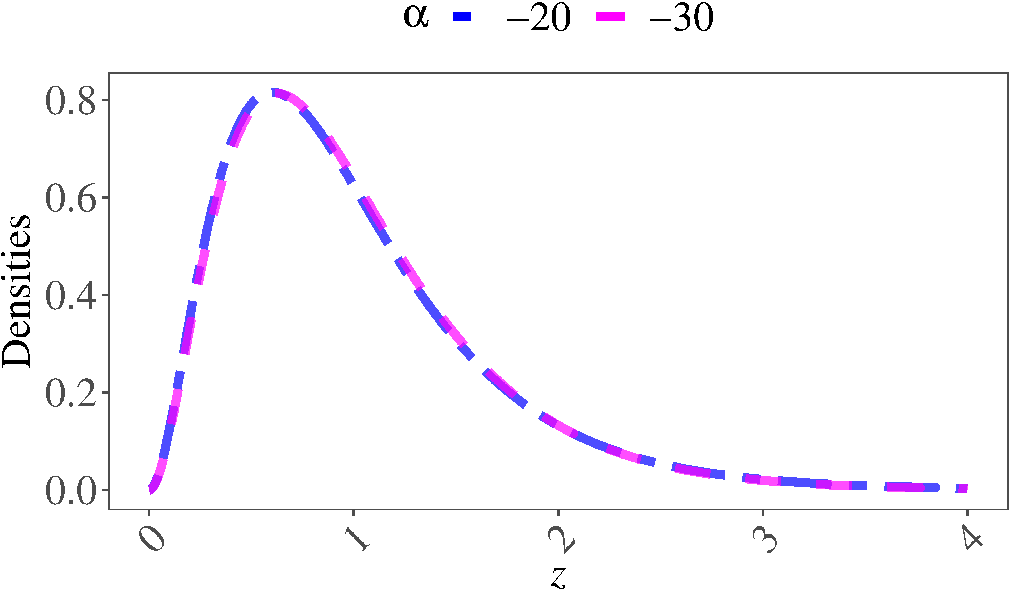
\includegraphics[width=.75\linewidth]{DensidadGI0L3}}
\subfigure[$L=8$]{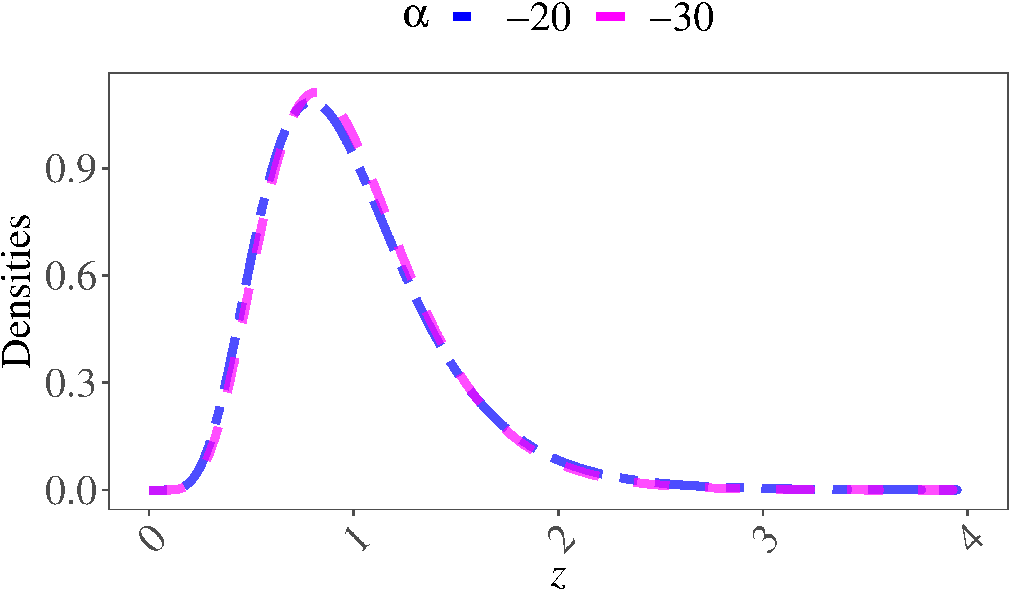
\includegraphics[width=.75\linewidth]{DensidadGI0L8}}
\caption{$\mathcal{G}^0(\alpha,\gamma^*,L)$ densities.}\label{densidades} 
\end{figure}
%JC Programa DensitiesGI02.R Es el mismo programa para L=3 y L=8. Tenès que cambiar el valor de L

Many methods of image filtering and edge detection use sliding masks to estimate parameters. 
These mask are usually of size $3 \times 3$, $5 \times 5$, $7 \times 7$, $9 \times 9$ and $11 \times 11$. 
For this reason, we chose $n=9,25,49,81$ and $121$ as the sample sizes to perform the empirical analysis.

%    It should be noted that it is of interest to find a texture parameter estimator that behaves well for small sample sizes. This aspect is interesting because many methods of image filtering or edge detection use sliding masks to estimate parameters. These mask are usually of size $3 \times 3$, $5 \times 5$, $7 \times 7$, $9 \times 9$ and $11 \times 11$.
%    
First of all, we evaluate the performance of the $\Gamma$, LN, and IG kernels studying MISE and the percentage of non-convergence cases, in order to choose the kernel that produces the best fits of the data. 
We use the LSCV method to find the bandwidth, and, for IG kernel, we also review the empirical bandwidth ($\text{IG}_{\text{E}}$) studied in Ref.~\cite{gambini2015}. 

Table~\ref{pp} shows the values of $\widehat{\text{MISE}}$ and non-convergence percent. 
It can be seen that IG and $\text{IG}_{\text{E}}$ present MISE values of several orders of magnitude higher than the other kernels. 
The same happens for non-convergence cases. 
The IG kernel has the highest percentage of these cases compared to the $\Gamma$ and LN kernel.

\begin{table}[hbt]  
\addtolength{\tabcolsep}{-3pt}
\caption{Estimated MISE and percentage of non-convergence cases for $L=3$.}\label{pp} 
\centering                                    
\begin{tabular}{c c S[table-format=2.2]S[table-format=2.2]S[table-format=2.2] S[table-format=2.2] @{\hskip 4mm} S[table-format=2.1]S[table-format=2.1]S[table-format=2.1]S[table-format=2.1]}                                    
	\toprule                                    
	& & \multicolumn{4}{c}{\multirow{2 }{*}{$\widehat{\text{MISE}}$}} & \multicolumn{4}{c}{\centering \% }\\
	&                          &                &               &         &     &   \multicolumn{4}{c}{non convergence cases}\\
	\cmidrule(lr){3-6}
	\cmidrule(lr){7-10}
	%\midrule
	
	$\alpha$		& $n$           & \mc{$\Gamma$} & \mc{LN}       & \mc{IG}     & \mc{$\text{IG}_{\text{E}}$}    & \mc{$\widehat{\alpha}_{\Gamma}$} & \mc{$\widehat{\alpha}_{\text{{LN}}}$}    & \mc{$\widehat{\alpha}_{\text{{IG}}}$} & \mc{$\widehat{\alpha}_{\text{{IG}}_{\text{E}}}$}\\
	\cmidrule(lr){1-2}
	\cmidrule(lr){3-6}
	\cmidrule(lr){7-10}                
	\multirow{5 }{5mm}{$-1.5$} 
	&  9       &       0.41     &     0.81     &     6.12      &     41.33     &    0     &    0.4      &    0.4       &    0 \\        
	&  25      &       0.12     &     0.18     &     2.46      &     17.02     &    0     &    0        &    0        &    0 \\
	&  49      &       0.08     &     0.54     &     1.16      &      9.67     &    0     &    0        &    0        &    0 \\
	&  81      &       0.06     &     0.08     &     0.75      &     6.13      &    0     &    0        &    0        &    0 \\
	&  121     &       0.06     &     0.08     &     0.53      &     4.00      &    0     &    0        &    0        &    0 \\
	\cmidrule(lr){3-6}
	\cmidrule(lr){7-10}                                    
	\multirow{5 }{5mm}{$-3$}    
	&  9       &       0.25     &     0.56     &     12.48     &     50.02     &    5.2    &    7.2     &   8         & 6.8 \\                    
	&  25      &       0.08     &     0.11     &     3.22      &     25.40     &    0.2    &    1       &    0.6      & 0.6 \\        
	&  49      &       0.04     &     0.07     &     0.69      &     16.40     &    0      &    0.4     &    0        &    0 \\
	&  81      &       0.03     &     0.03     &     0.25      &     11.58     &    0      &    0       &    0        &    0 \\
	&  121     &       0.02     &     0.03     &     0.17      &     8.98      &    0      &    0       &    0        &    0 \\    
	
	\cmidrule(lr){3-6}
	\cmidrule(lr){7-10}                                       
	\multirow{5 }{5mm}{$-5$}    
	&  9       &       0.24     &     0.43     &     15.32     &     63.38     &    9.6    &    13.2    &   17         &    13.2 \\                    
	&  25      &       0.07     &     0.09     &     4.65      &     32.94     &    3.4    &   5        &    2         &    1.6 \\                    
	&  49      &       0.04     &     0.06     &     0.68      &     24.41     &    1.4    &    1.2     &    1         &    0.4 \\
	&  81      &       0.03     &     0.03     &     0.29      &     18.91     &    0.4    &    0.8     &    0.2       &    0 \\
	&  121     &       0.02     &     0.02     &     0.18      &     15.92     &    0      &    0.2     &    0         &    0 \\
	
	\cmidrule(lr){3-6}
	\cmidrule(lr){7-10}                                        
	\multirow{5 }{5mm}{$-8$}    
	&  9       &       0.24     &     0.38     &     18.11     &     73.08     &    16.6    &    19     & 26.2         &    18 \\                
	&  25      &       0.07     &     0.11     &     5.13      &     40.48     &    81.8    &   11      &    8.8       &    4.2 \\            
	&  49      &       0.04     &     0.05     &     0.93      &     30.23     &    5       &    5.4    &    4.2       &    1.2 \\    
	&  81      &       0.03     &     0.03     &     0.33      &     25.71     &    4.4     &    4      &    2         &    0.2 \\    
	&  121     &       0.02     &     0.02     &     0.21      &     21.19     &    1.8     &    2      &    0.8       &    0.4 \\
	\bottomrule
\end{tabular}                                              
\end{table}    

Therefore, we chose $\Gamma$ and LN kernels to estimate the underlying density function.

The following analysis was performed through a Monte Carlo experiment, which consists of $500$ independent replications for each of several parameter values: 
$L\in\{3,8\}$ to consider multilook case,
$\alpha\in\{-1.5, -3, -5, -8\}$ to represent different levels of texture, 
and 
$n\in\{9, 25,49, 81,121,500\}$ to consider different scenarios of window sizes, and a large sample situation.

Although the variance of a $\mathcal{G}^0$-distributed random variable is infinite when $\alpha>-2$, cf.~\eqref{moments_gI0}, we need to assess the behavior of estimators in such cases.
As noted by, among others Ref.~\cite[Fig.~5]{LowCostRobustEstimationfortheSingleLookGI0ModelUsingtheParetoDistributioninpress}, one should expect that extremely heterogeneous samples as, for instance, those from urban areas, are described in this region of the parameter space.

Each replication produces estimates $\{\widehat{\alpha}_1, \dots, \widehat{\alpha}_{500}\}$ with which we compute 
the sample mean $\overline{\widehat{\alpha}}=(500)^{-1}{\sum_{i=1}^{500}{\widehat{\alpha}_i}}$, 
the sample bias $\widehat{B}(\widehat\alpha) = \overline{\widehat\alpha}- \alpha$, 
and 
the sample mean squared error $\widehat{\operatorname{mse}}=({500})^{-1}{\sum_{i=1}^{500}{(\widehat{\alpha}_i-\alpha)^2}}$.


We compare four estimators for the multilook case: 
$\widehat{\alpha}_{\text{{ML}}}$, 
$\widehat{\alpha}_{\text{{LC}}}$, 
$\widehat{\alpha}_{\Gamma}$ ($\Gamma$ kernel) and $\widehat{\alpha}_{\text{{LN}}}$ (LN kernel).

The performance of the proposed techniques is assessed twofold: in pure and contamination cases. 
%Through the Monte Carlo experiment, we evaluate the bias and the mean squared error in different stages. 
We also assess the robustness of these estimators employing their Stylized Empirical Influence Functions (SEIFs) and contaminating the data, as explained in subsection~\ref{robustez}. 
The estimators were also evaluated in terms of the percentage of situations for which there was no convergence, and by their computational cost. 
For $\widehat{\alpha}_{\text{{LN}}}$ we also account, as a case of non-convergence, for situations where no solution was found for equation~\eqref{eq:logm}.


\subsection{Computational Information}

Table~\ref{NoConvMLyNGyLNyLC_L=3} shows the percentage of non-convergence cases for $L=3$; the situation for $L=8$ yields similar values and, thus, is not reported for brevity.
It can be seen that the $\widehat{\alpha}_{\text{{ML}}}$ and $\widehat{\alpha}_{\text{{LC}}}$ estimators have the highest values of lack of convergence followed by  $\widehat{\alpha}_{\text{{LN}}}$ and $\widehat{\alpha}_{\Gamma}$.

\begin{table}[hbt]
\caption{Percentage of non-convergence cases,  $L=3$.}\label{NoConvMLyNGyLNyLC_L=3}
\centering
\begin{tabular}{c*6{r}}
	\toprule        
	$\alpha$ & $n$ & $\widehat{\alpha}_{\text{{ML}}}$ & $\widehat{\alpha}_{\Gamma}$ & $\widehat{\alpha}_{\text{{LN}}}$ &  $\widehat{\alpha}_{\text{{LC}}}$\\
	\cmidrule(lr){1-2}\cmidrule(lr){3-6}
	\multirow{2 }{*}{$-1.5$} 
	&   $9$ & $0$ & $0$ & $0.4$ &  $2.8$\\
	&  $25$ & $0$ & $0$ & $0$ & $0.2$\\
	\cmidrule(lr){1-2}\cmidrule(lr){3-6}
	\multirow{5 }{*}{$-3$} 
	&   $9$ & $13$    & $5.2$  & $7.2$  &  $28.4$\\ 
	&  $25$ & $1$     & $0.2$  & $1$    &  $11.4$\\
	&  $49$ & $0.2$   & $0$    & $0.4$  & $3.8$\\ 
	&  $81$ & $0$     & $0$    & $0$    & $2.4$\\ 
	& $121$ & $0$     & $0$    & $0$    & $0.2$\\ 
	\cmidrule(lr){1-2}\cmidrule(lr){3-6}
	\multirow{5 }{*}{$-5$} 
	&   $9$ & $26.8$  & $9.6$  & $13.2$ &  $35.2$\\ 
	&  $25$ & $10$    & $3.4$  & $5$    & $28.6$\\ 
	&  $49$ & $3.4$   & $1.4$  & $1.2$  & $18.6$\\ 
	&  $81$ & $0.2$   & $0.4$  & $0.8$  & $15.8$\\ 
	& $121$ & $0.4$   & $0$    & $0.2$  & $9.6$\\ 
	& $500$ & $0$     & $0$    & $0$    & $0.6$\\ 
	\cmidrule(lr){1-2}\cmidrule(lr){3-6}
	\multirow{5 }{*}{$-8$} 
	&   $9$  & $39.6$ & $16.6$ & $19$   & $44.2$\\ 
	&  $25$  & $28.6$ & $9$    & $11$   & $36.4$\\ 
	&  $49$  & $18.4$ & $5$    & $5.4$  & $31.6$\\ 
	&  $81$  & $12$   & $4.4$  & $4$    & $27.2$\\ 
	& $121$  & $5.8$  & $1.8$  & $2$    & $24.6$\\ 
	& $500$  & $0$    & $0$    & $0.2$  & $9$\\
	\bottomrule     
\end{tabular}
\end{table}    

Such a lack of convergence is more pronounced for homogeneous ($\alpha=-8$) and textured ($\alpha=-5$) areas. 
This issue had been observed for amplitude data in~\cite{FreryCribariSouza:JASP:04} for $\widehat{\alpha}_{\text{{ML}}}$, and is related to the decreasing curvature of the likelihood function.

Table~\ref{tablaDeTiemposmediosMLyGAyLNyLC} shows the mean system time, in seconds, for five hundred replications for each estimator, considering $\alpha=-5$ and sample $n=81$. 
Albeit $\widehat{\alpha}_{\Gamma}$ and $\widehat{\alpha}_{\text{{LN}}}$ require much more processing time than the others estimators, the former fail to converge about half of the times that the last.

\begin{table}[hbt]
\caption{Mean system time for uncontaminated data, $L=3$ and $n=81$. }
\label{tablaDeTiemposmediosMLyGAyLNyLC}
\centering
\begin{tabular}{cccc}
	\toprule
	ML& $\Gamma$ & LN & LC \\
	\cmidrule(lr){1-4}
	$0.003$& $1.87$ & $1.87$ &$0.003$ \\
	\bottomrule
\end{tabular}

\end{table}

\subsection{Simulation Results -- Pure Cases}

Figure~\ref{SesgoyECMSinContL=3} shows the bias and mean square error (MSE) for uncontaminated data, $L=3$, and varying sample size. 
The results are shown in the semilogarithm scale. 
The iterations considered are those where all methods converge. 

We also plot the confidence interval of approximately \SI{95}{\percent} level for each estimate, using the percentile method described in Ref.~\cite{Buckland1983}. 
This method consists in using the percentile $(\alpha/2)$ and $(1-\alpha/2) $ of the distribution of $\widehat{\alpha}$. 
This method was evaluated by~\cite{Buckland1983} in the case where the underlying distribution is exponential, where the symmetry of the distribution fails. 
The author shows that this interval has a better performance than using the normal approximation. 

It can be seen that, for a fixed $n$ and as $\alpha$ decreases, both  $\widehat{\text{Bias}}$ and $\widehat{\text{MSE}}$ increase in most methods. 
It is important to note that $\widehat{\alpha}_{\text{{ML}}}$ and $\widehat{\alpha}_{\text{{LC}}}$ on the one hand, 
and $\widehat{\alpha}_{\Gamma}$ and $\widehat{\alpha}_{\text{{LN}}}$ on the other hand, have similar behavior in both bias and MSE in most cases. 
This similar behavior can also be observed in the confidence intervals: $\widehat{\alpha}_{\text{{ML}}}$ and $\widehat{\alpha}_{\text{{LC}}}$ produce wider intervals than the other estimators, showing that they are less accurate than MDE.

For extremely heterogeneous $(\alpha > -3)$ and heterogeneous areas $(\alpha \in (-6,-3])$, the MDE estimators have a better performance than the rest. 
For moderately heterogeneous areas, all methods have similar behavior; however, MDE has a lower MSE. 
For homogeneous areas, $\widehat{\alpha}_{\text{{ML}}}$ is the one with the smallest bias, although the MSE is comparable to the MDE estimators except for moderate size samples where the MSE is the largest.

\begin{figure*}[hbt]
\centering
\subfigure[\label{SesgoSinContL=3}$\widehat{\text{Bias}}$]{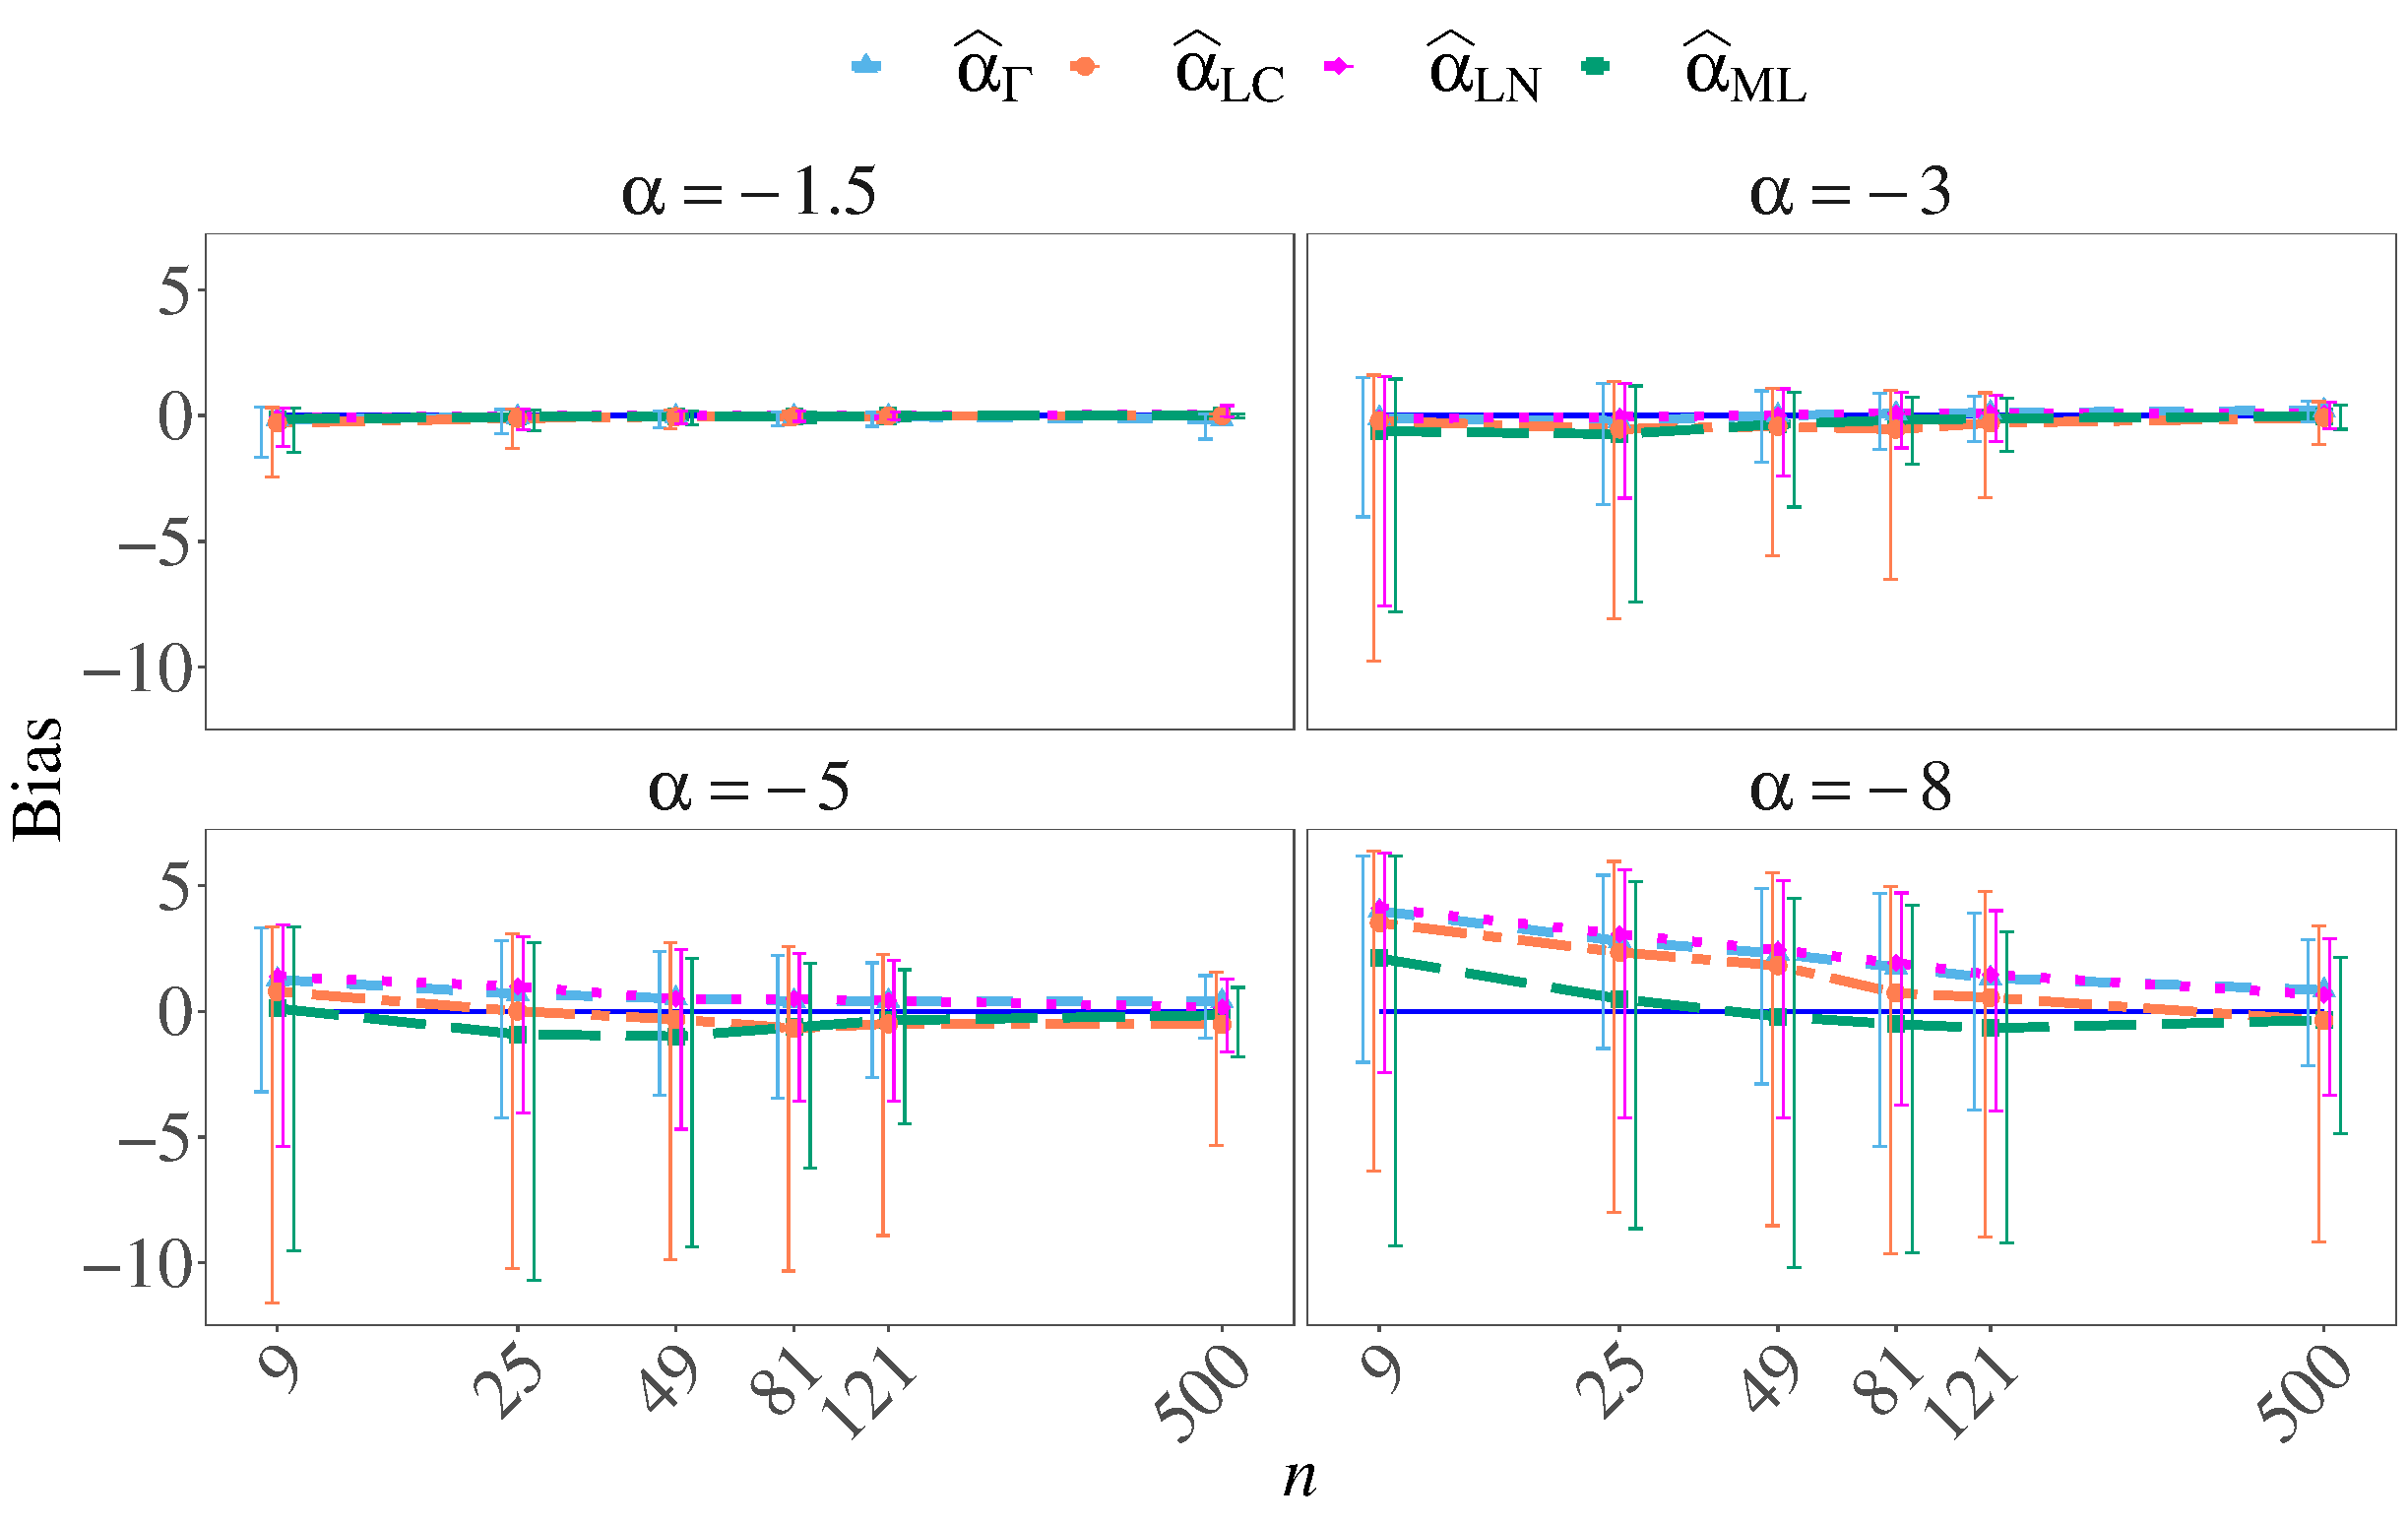
\includegraphics[width=0.49\linewidth]{GraficoSesgoMVyGAyLNyLC_L=3SinCont_BarrasErroryPercentil}}
\subfigure[\label{ECMSinContL=3}$\widehat{\text{MSE}}$]{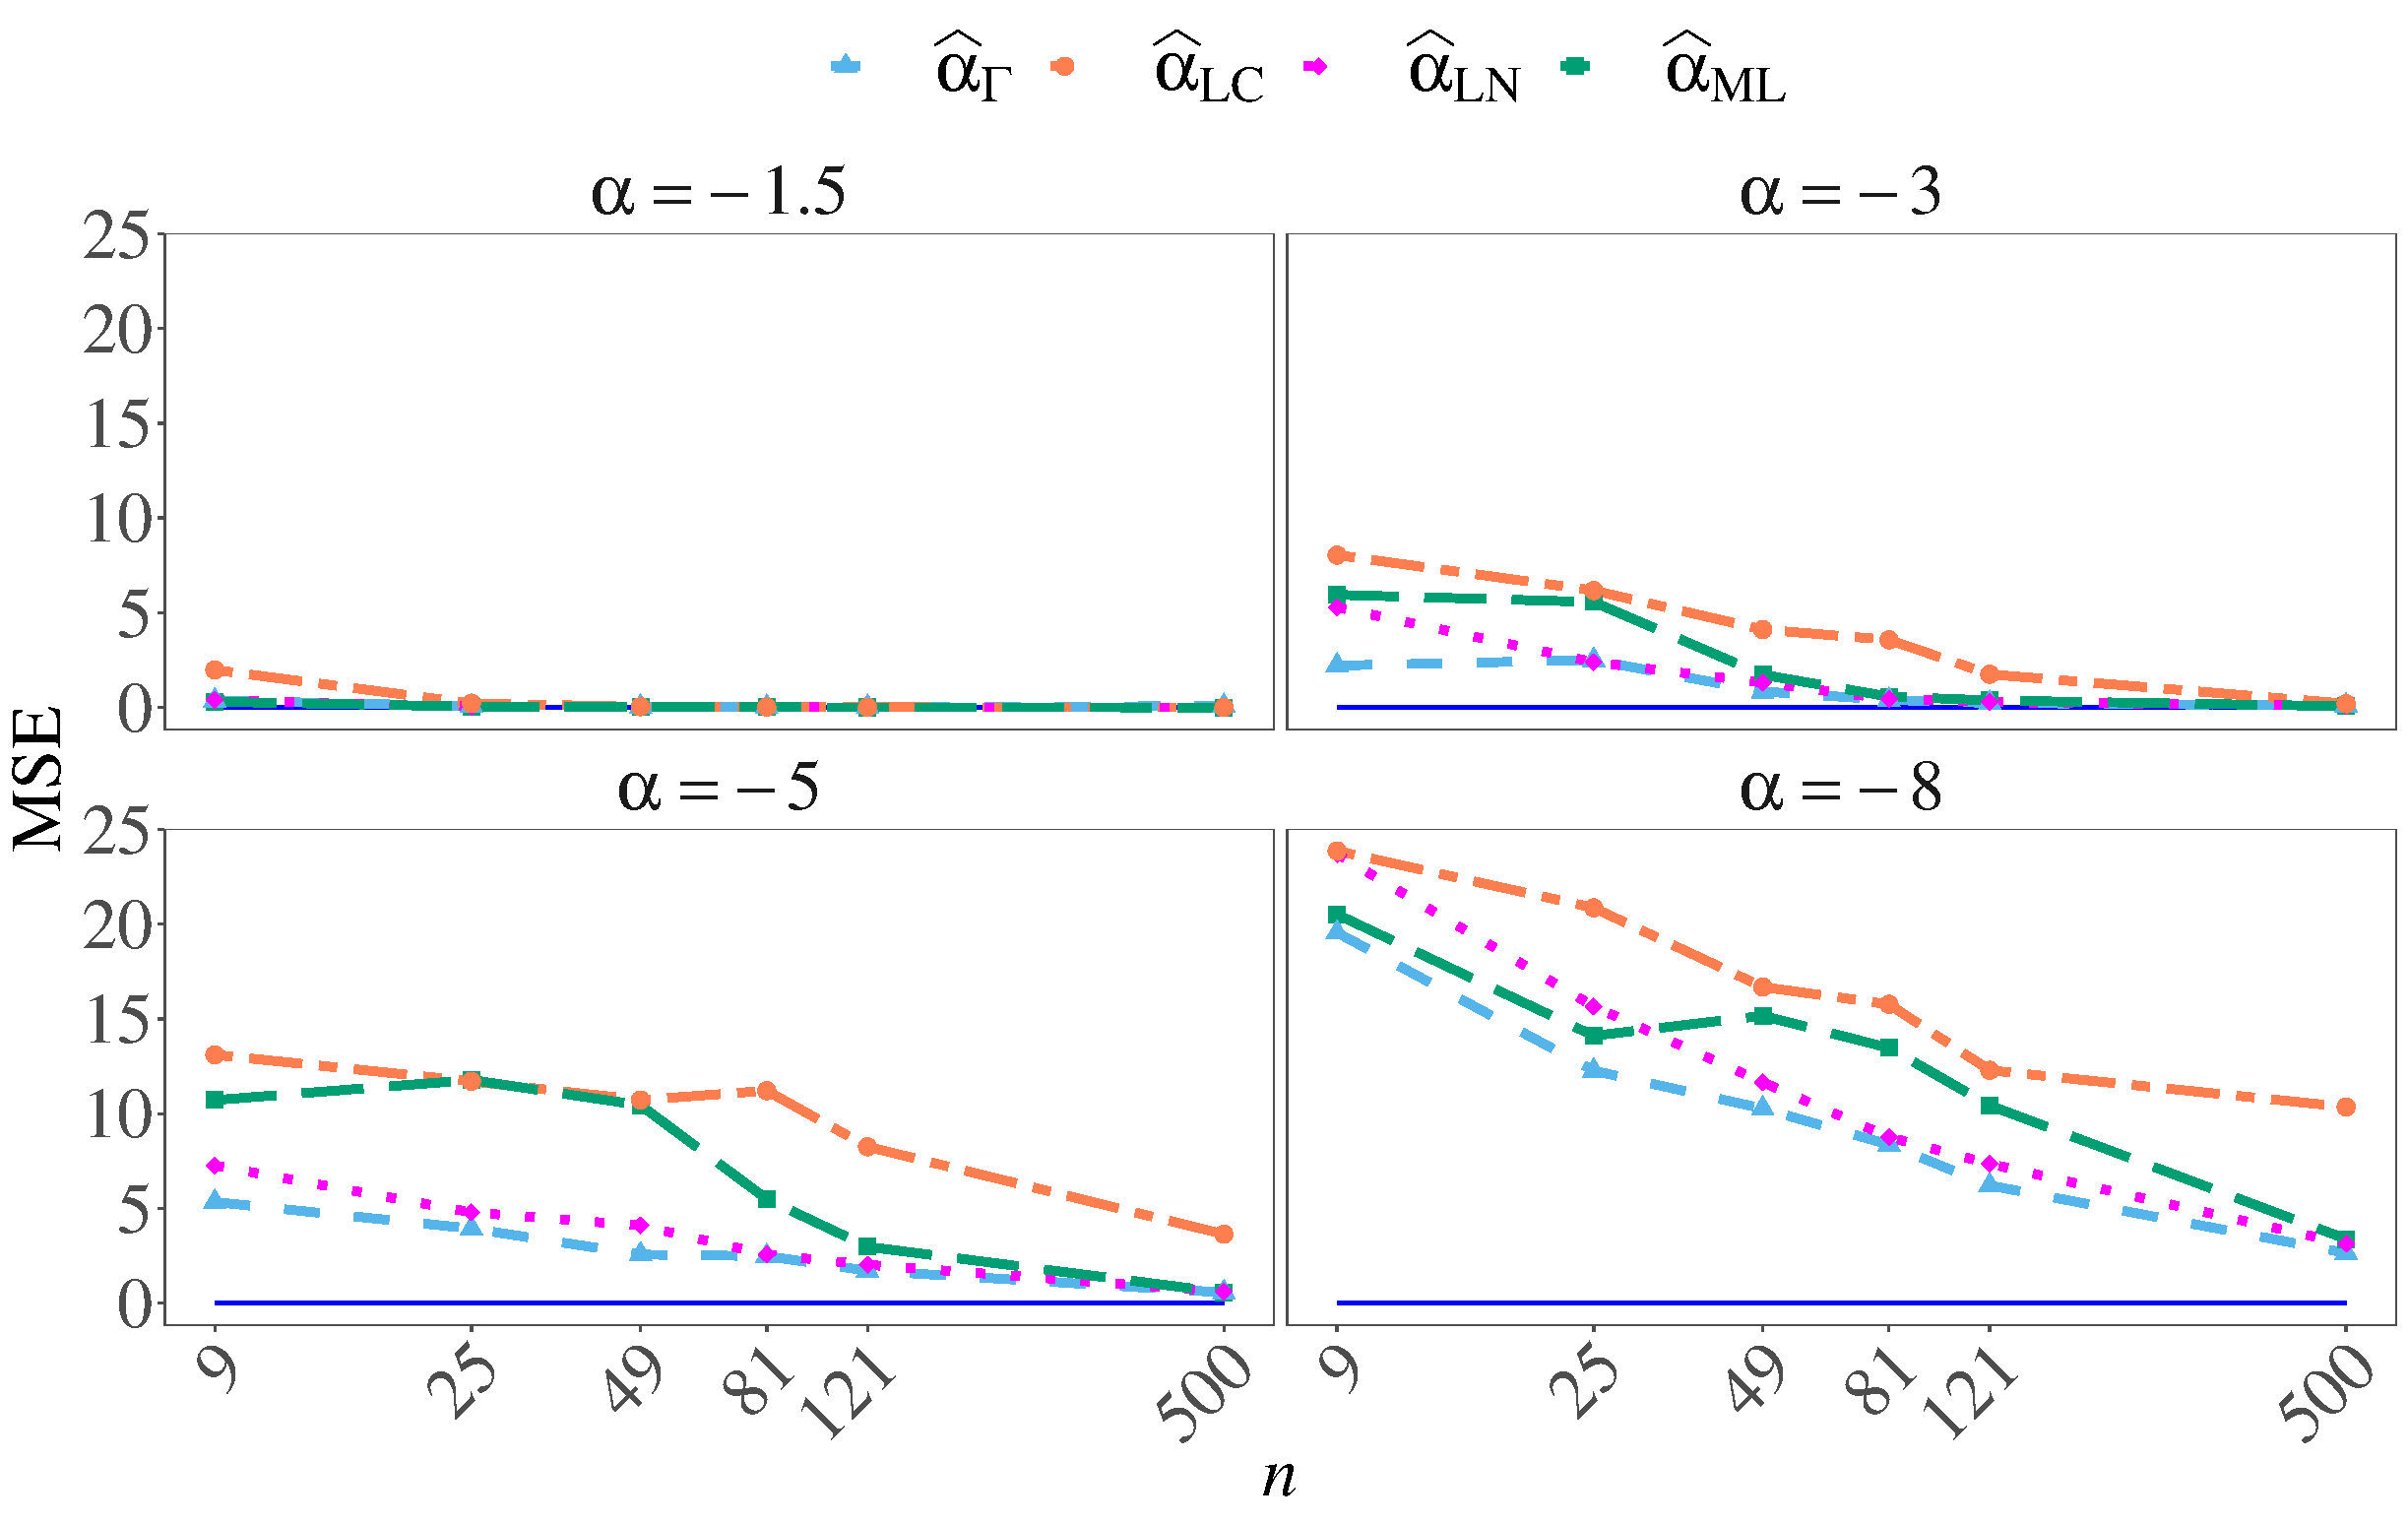
\includegraphics[width=0.49\linewidth]{GraficoECMMVyGAyLNyLC_L=3SinCont_BarrasErroryPercentil}}
\caption{Sample Bias and MSE with uncontaminated data and $L=3$.}\label{SesgoyECMSinContL=3} 
\end{figure*}    
%JC Programa: GraficoSesgoSinCont_L3BarrasErroryPercentil.R

A similar analysis was done for the case $L=8$. Figs.~\ref{SesgoSinContL=8} and~\ref{ECMSinContL=8} show that $\widehat{\alpha}_{\text{{ML}}}$ has the best performance for homogeneous
areas in terms of bias, while $\widehat{\alpha}_{\text{{LN}}}$ outperforms the rest in extremely textured areas and with moderate texture.

\begin{figure*}[hbt]
\centering
\subfigure[\label{SesgoSinContL=8}$\widehat{\text{Bias}}$]{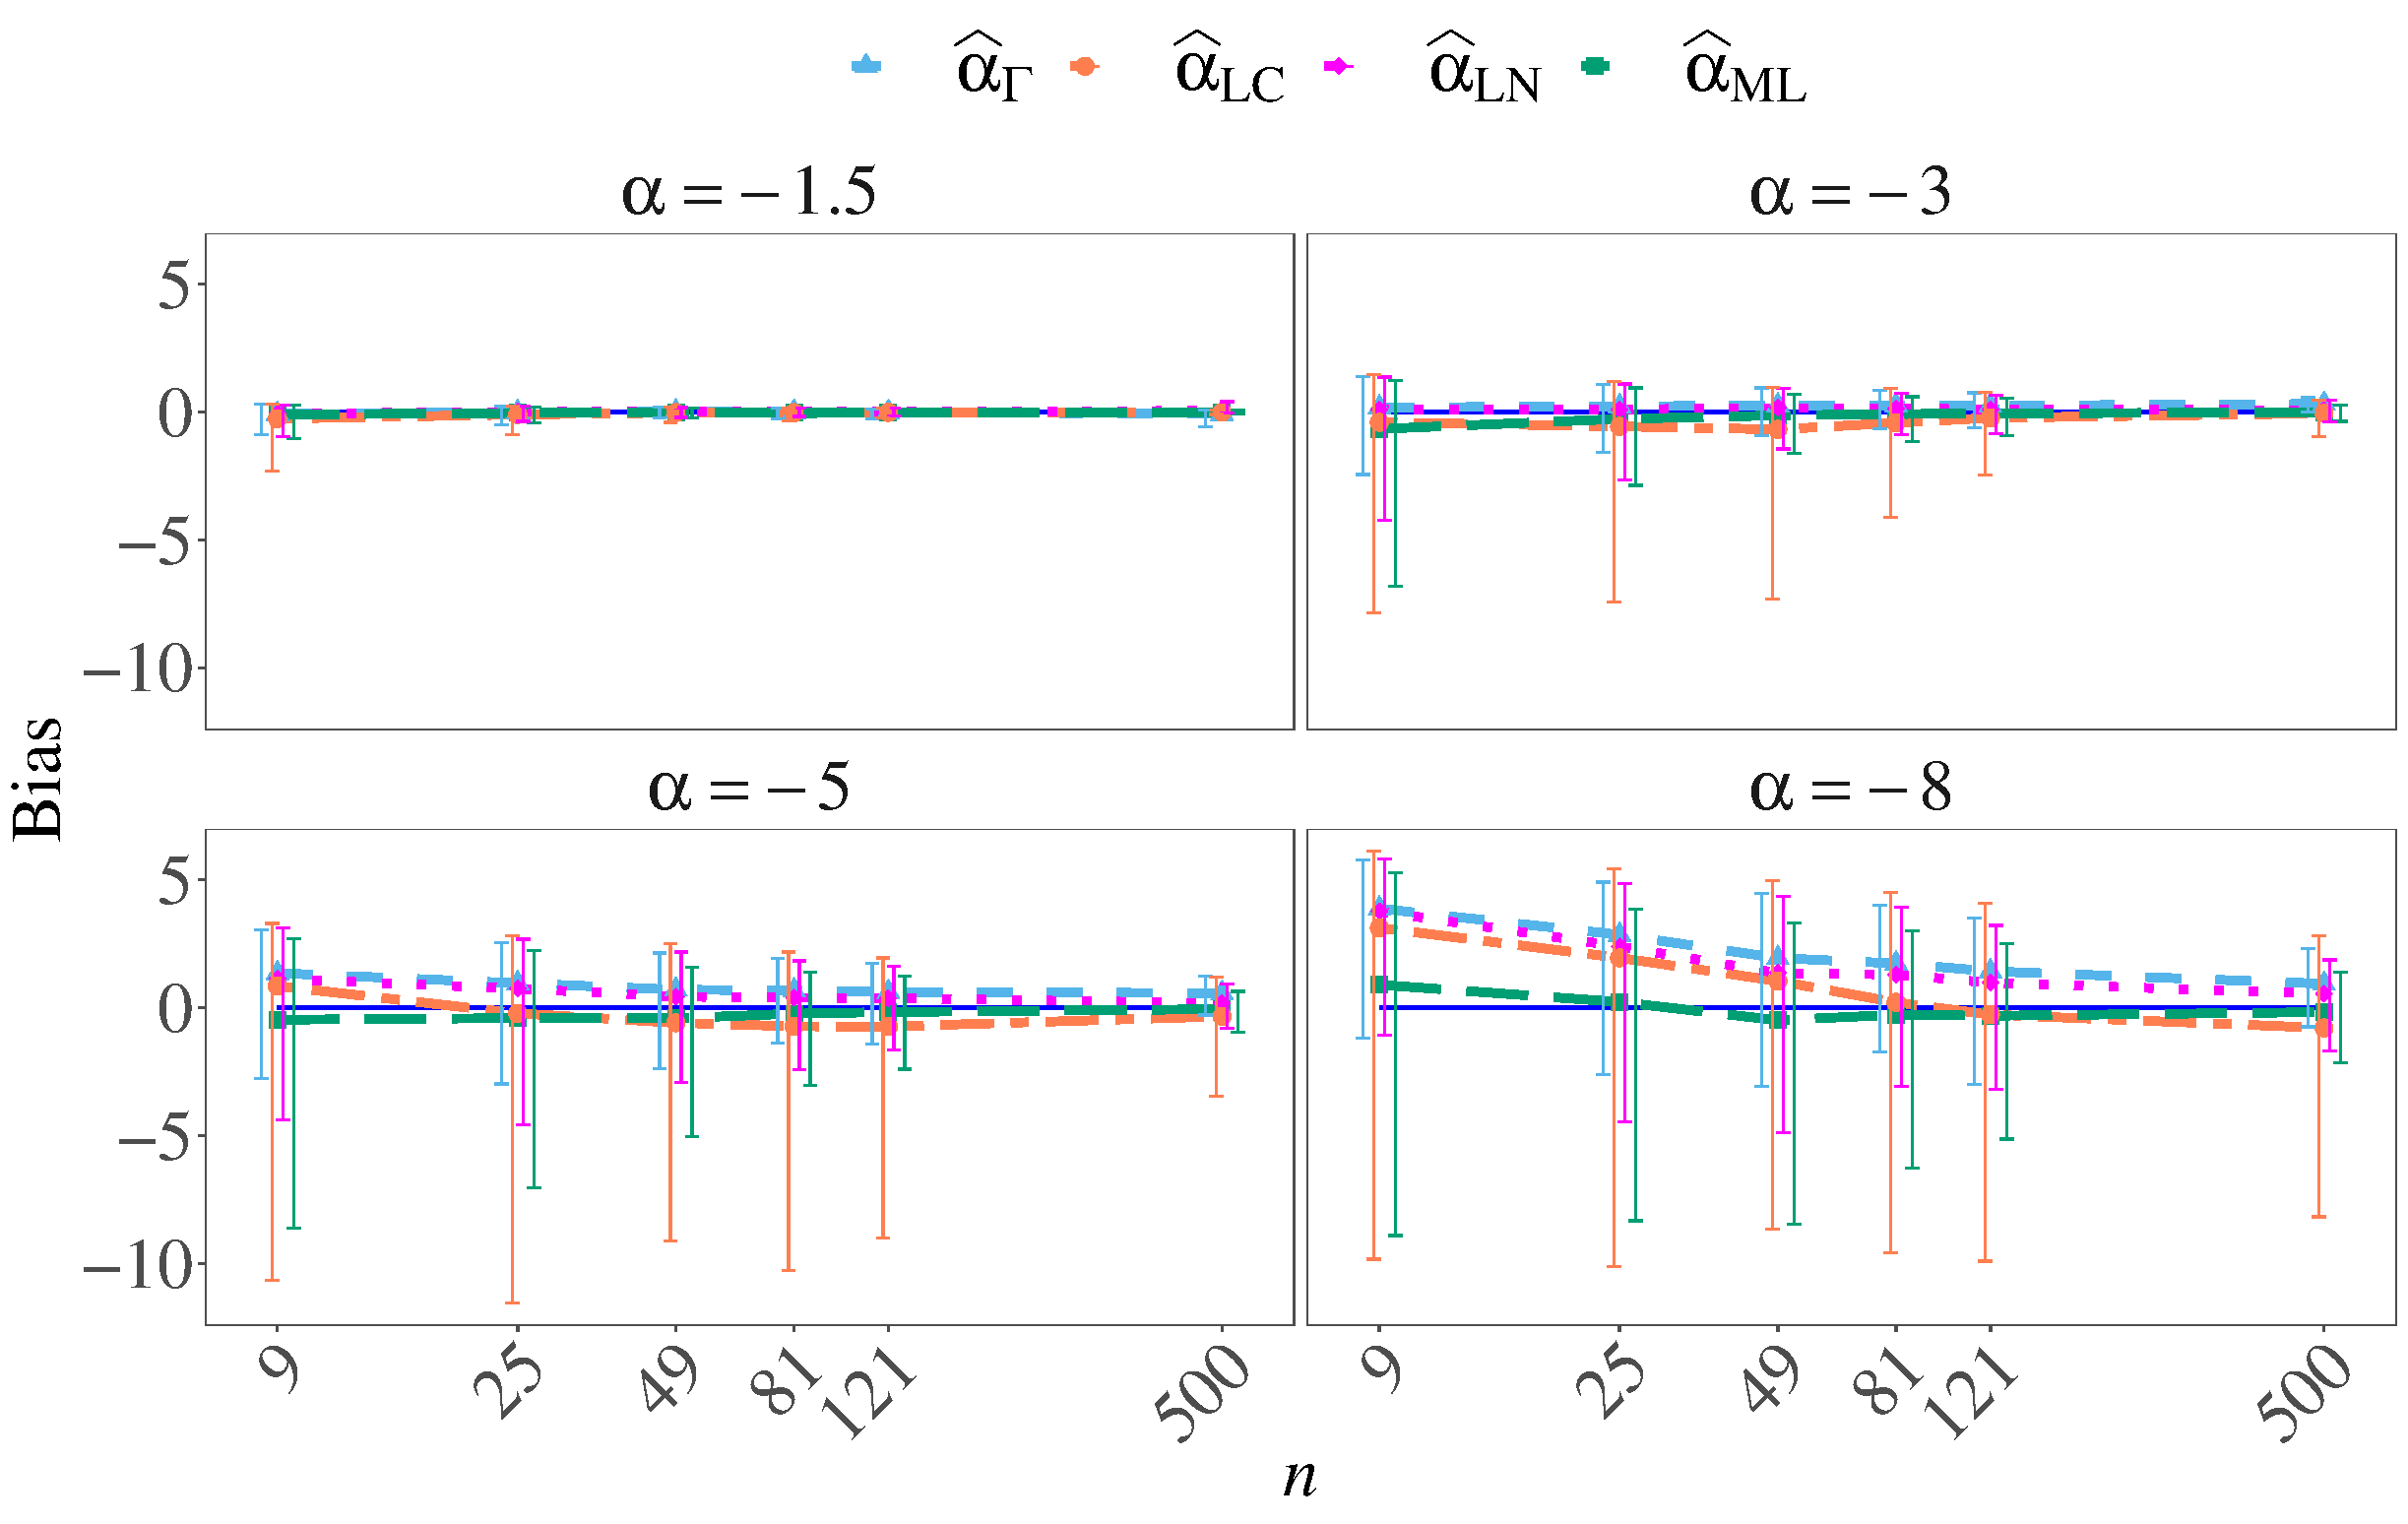
\includegraphics[width=0.49\linewidth]{GraficoSesgoMVyGAyLNyLC_L=8SinCont_BarrasErroryPercentil}}
\subfigure[\label{ECMSinContL=8}$\widehat{\text{MSE}}$]{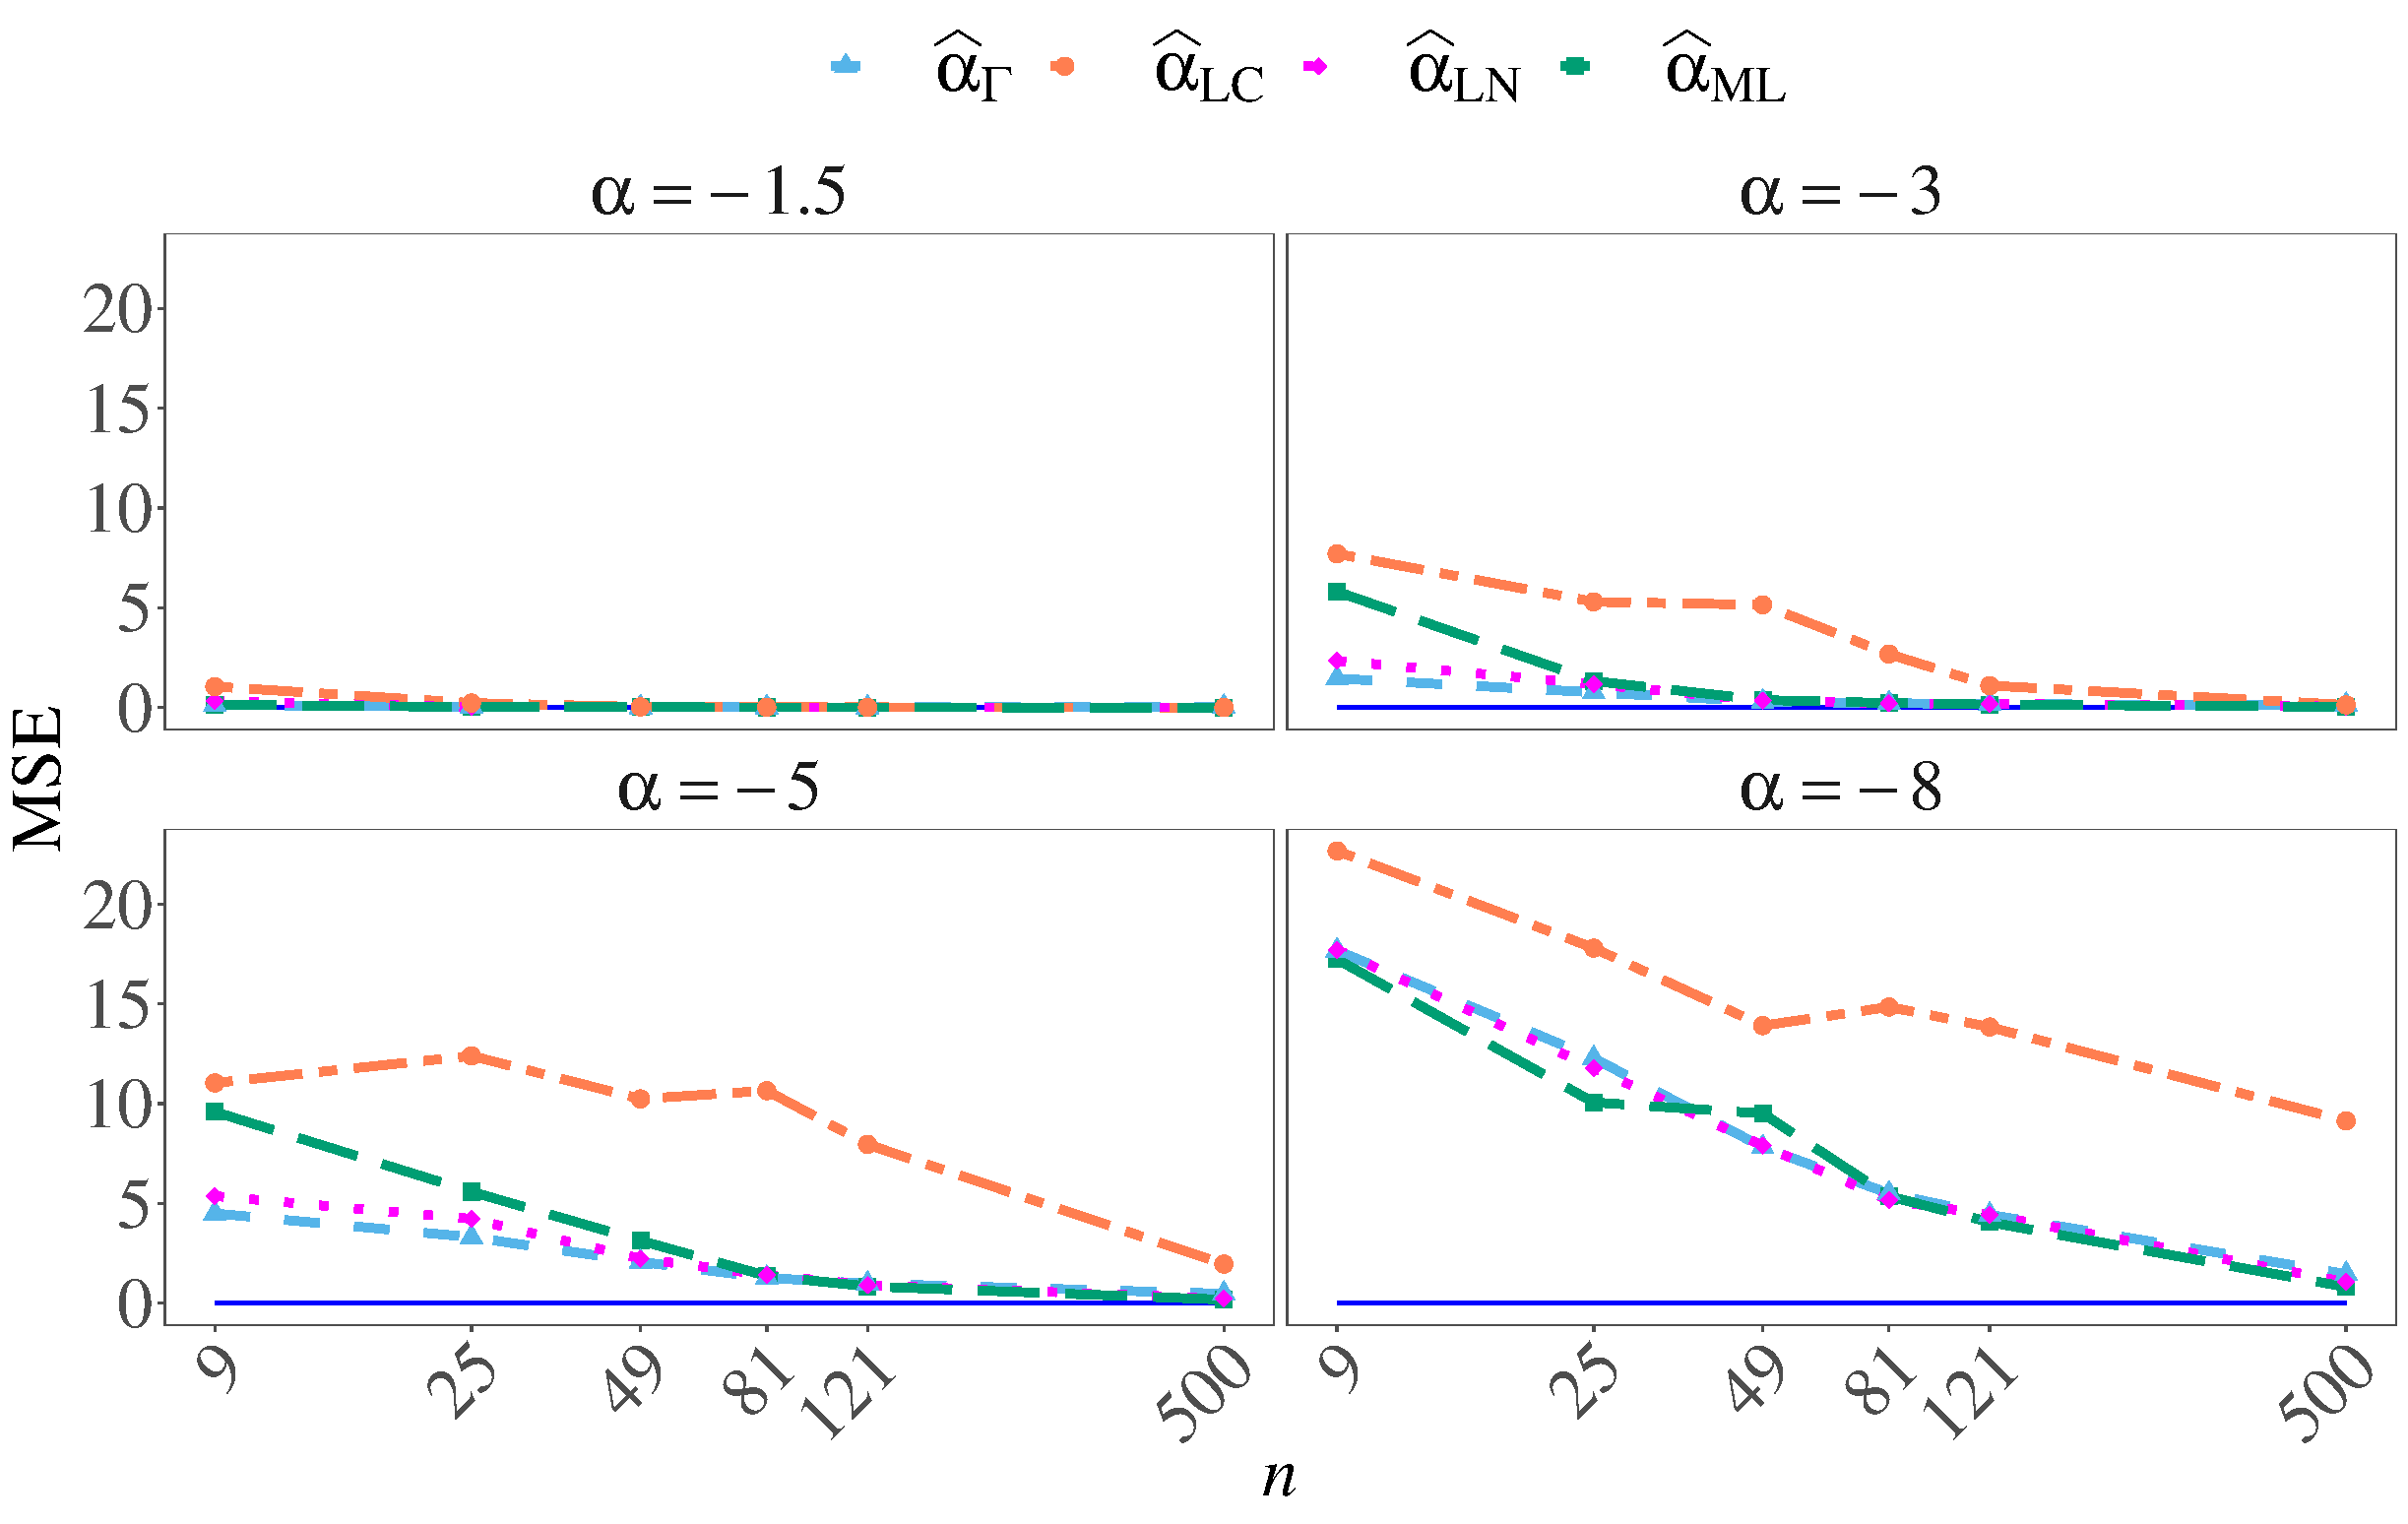
\includegraphics[width=0.49\linewidth]{GraficoECMMVyGAyLNyLC_L=8SinCont_BarrasErroryPercentil}}
\caption{Bias and MSE estimates for uncontaminated data and $L=8$.}\label{SesgoyECMSinContL=8} 
\end{figure*}
%JC Programa: GraficoSesgoSinCont_L8BarrasErroryPercentil.R


Fig.~\ref{Fig:DistributionL=3_alfa=-3} shows estimates of the density of these estimators for $\alpha=-3$ and $L=3$. 
As the sample size increase, the mean of these estimators approaches the true value of the texture parameter, and their distributions become more symmetric. 
Moreover, from $n=49$ onwards the shape of the $\widehat{\alpha}_{\text{{LN}}}$ distribution is very similar to that of $\widehat{\alpha}_{\text{{ML}}}$.

\begin{figure}[hbt]
\centering
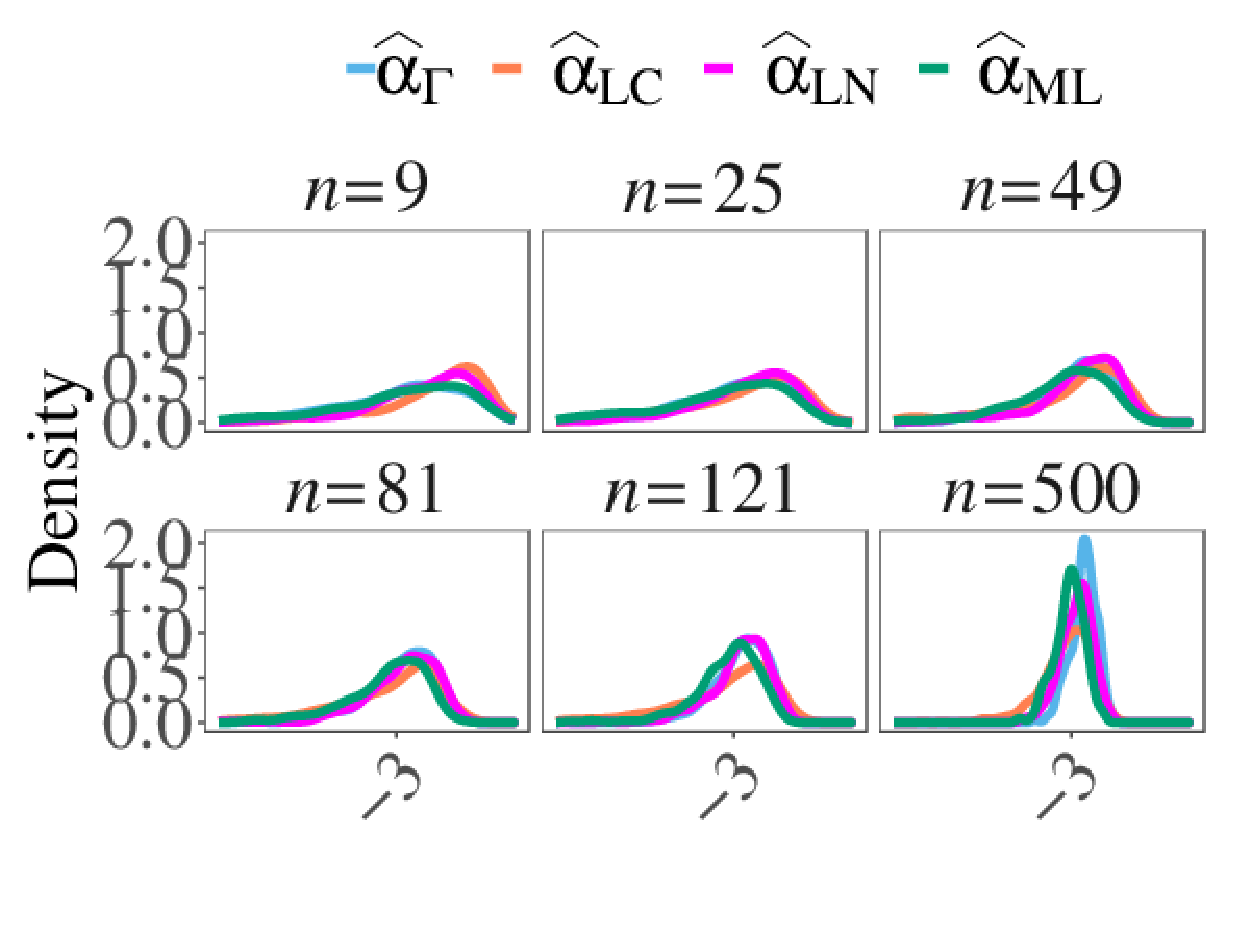
\includegraphics[width=1\linewidth]{DensidadEstimadorNoCont}
\caption{\label{Fig:DistributionL=3_alfa=-3} Sample density of estimators for $\alpha=-3$ and  $L=3$ }
\end{figure}
%JC Programa:DensityPropuestaNoCont.R	

In order to investigate the asymptotic behavior of these estimators, we studied estimates of their density functions for $n=500$ and all the texture parameters. 
The result of this analysis is shown in Fig.~\ref{Fig:Densities_n500}, where
the vertical blue lines indicate the true value. 
Notice that the ranges of the $y$-axis are different among the plots. 
The heavytailnedess of these densities is noticeable.
For $\alpha=-1.5$, all are quite concentrated around the true parameter value. 
As the texture parameter reduces, the densities more spread.
This issue has been previously noted in Refs.~\cite{APSAR2013ParameterEstimationStochasticDistances,CribariFrerySilva:CSDA,AllendeFreryetal:JSCS:05,FreryCribariSouza:JASP:04}, among others.
The estimator which suffers the least with the texture reduction is $\widehat{\alpha}_{\text{{ML}}}$, due to its optimal asymptotic properties.      

\begin{figure}[hbt]
\centering
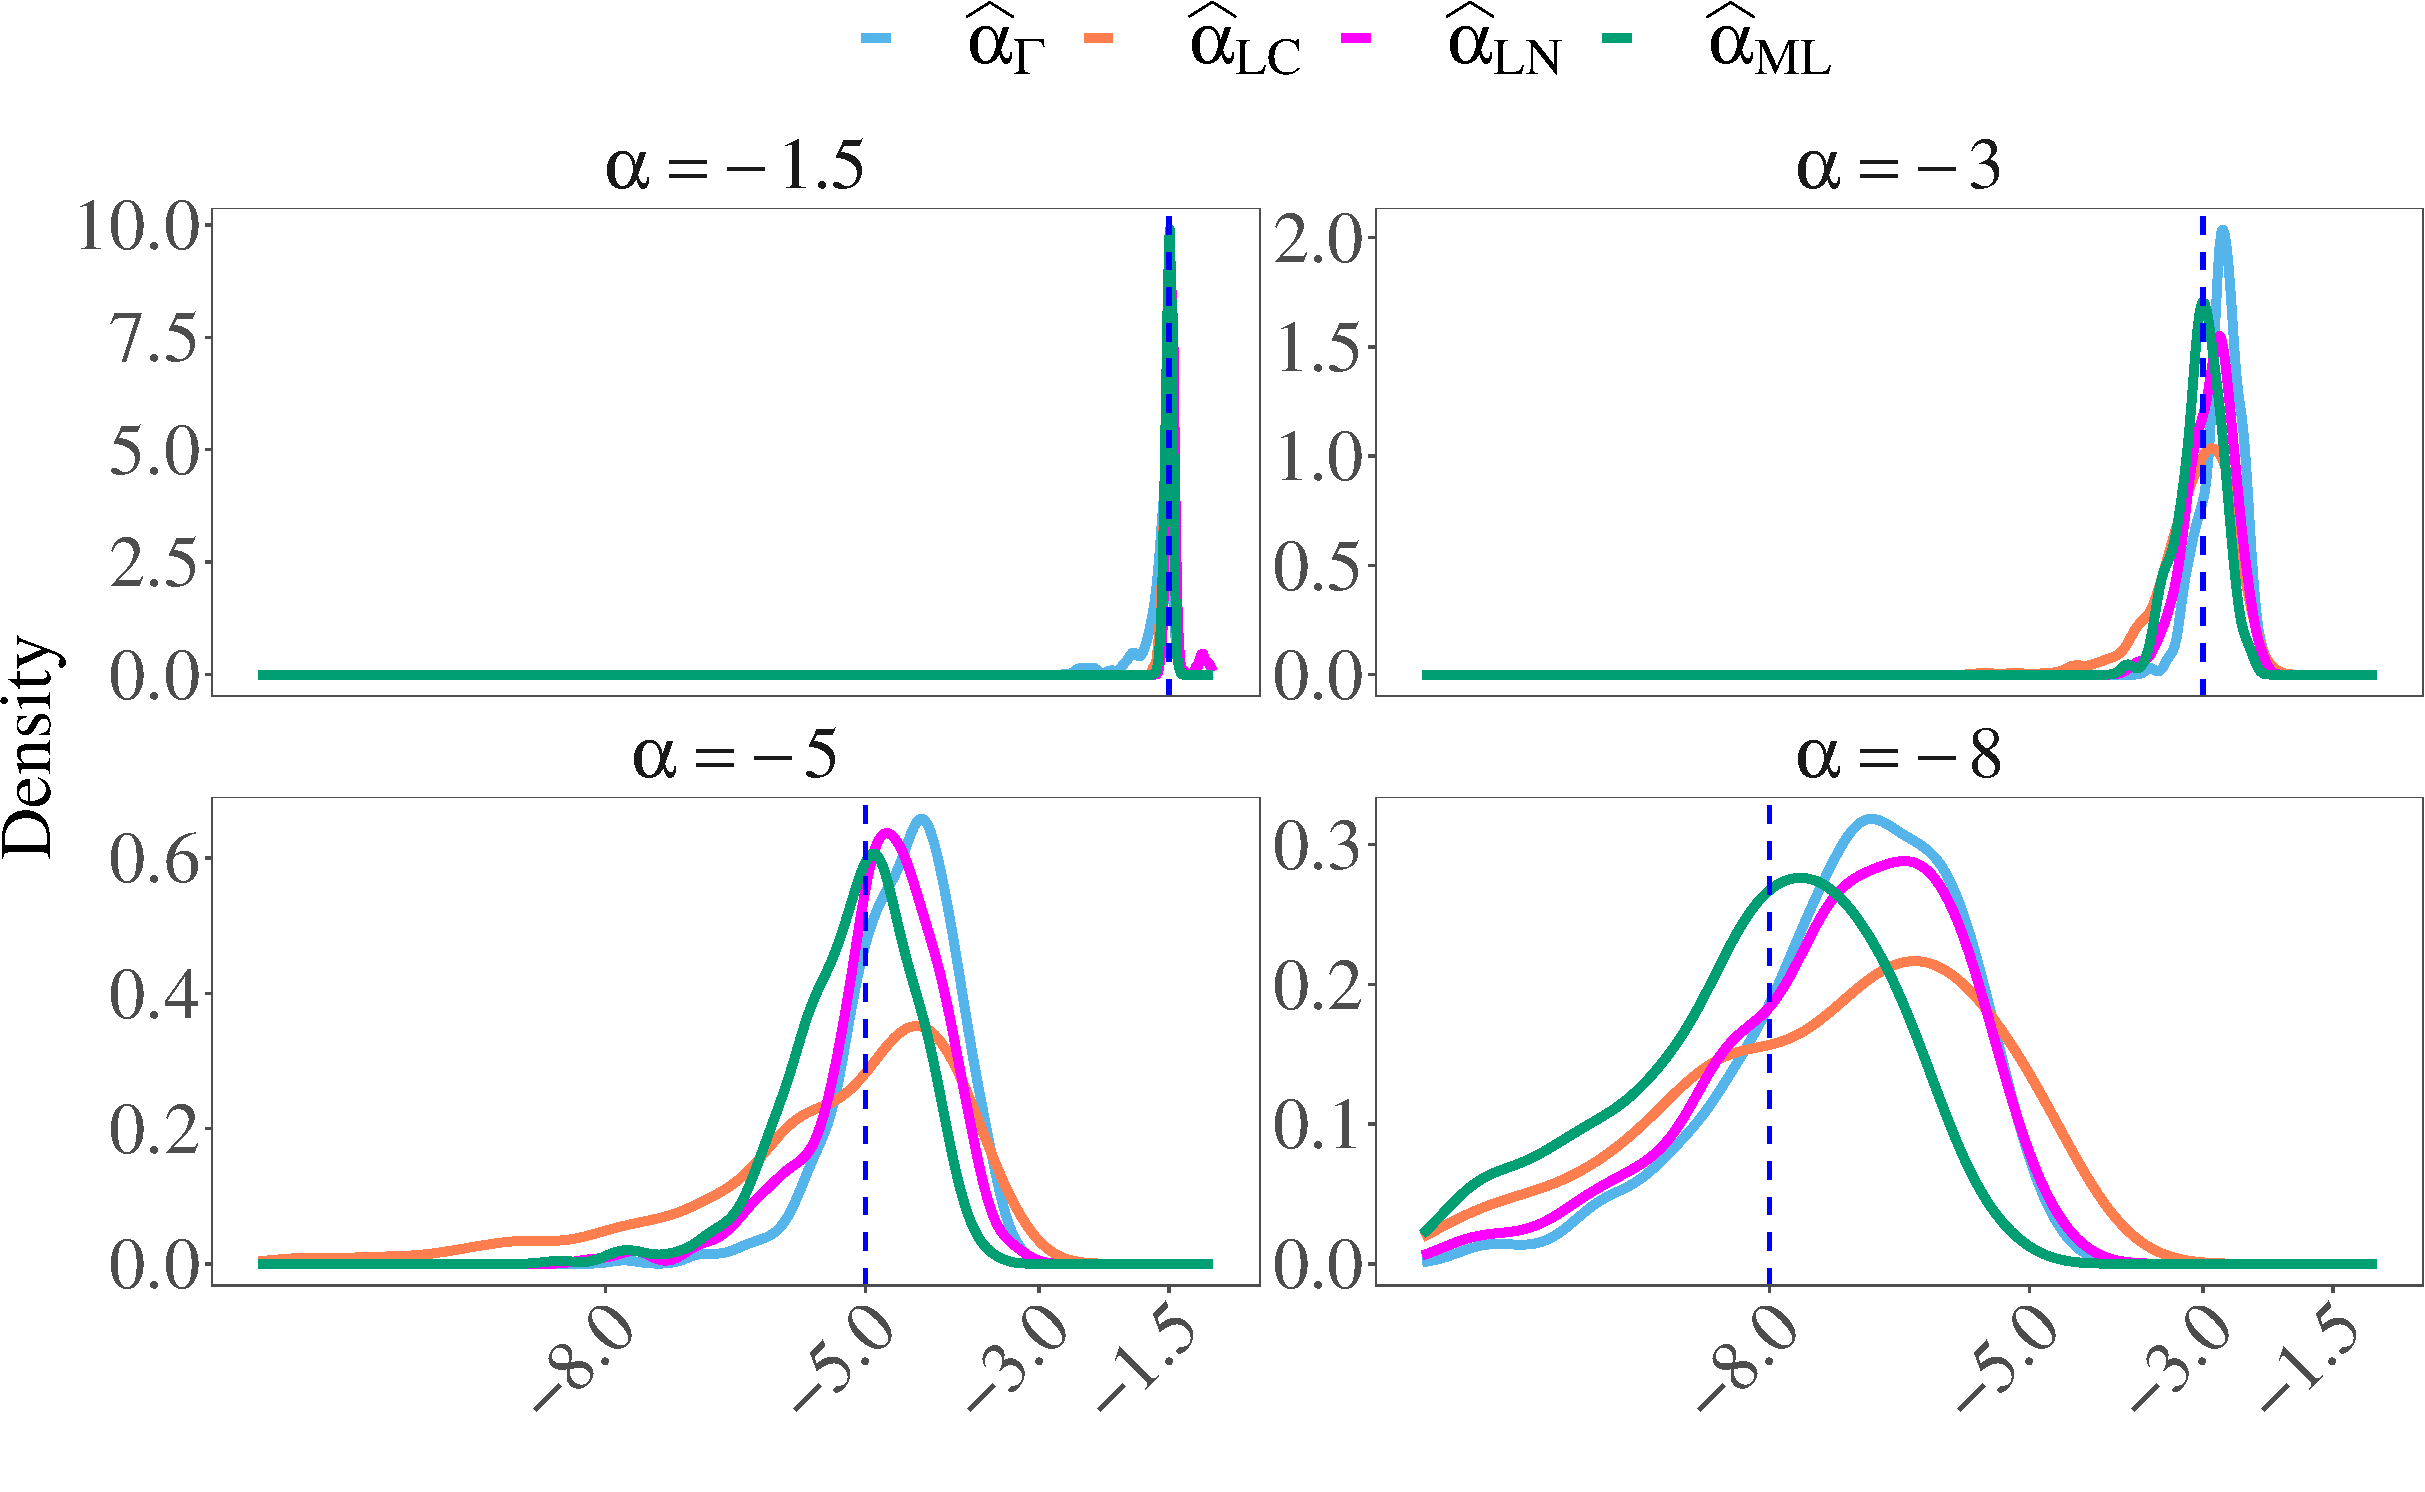
\includegraphics[width=1\linewidth]{Asymptotic_n500_TodoAlfa}
\caption{\label{Fig:Densities_n500} Sample density of the estimators for $n=500$. }
\end{figure}
%JC Programa:AsymptoticDensityNoCont_n500.R	

Table~\ref{tab:SkewKurt} presents the skewness and kurtosis values for simulated data and $L=3$. 
The skewness is negative in all the cases, except for $\alpha=-1.5$ and $n=121,500$ for the $\widehat{\alpha}_{\text{{LN}}}$ estimator. 
As the sample size increases, the skewness decreases in absolute value. 
For textured and homogeneous areas $\widehat{\alpha}_{\text{{ML}}}$, $\widehat{\alpha}_{\Gamma}$ and $\widehat{\alpha}_{\text{{LN}}}$ present similar asymmetry. 
In extremely textured areas, $\widehat{\alpha}_{\text{{ML}}}$ and $\widehat{\alpha}_{\text{{LC}}}$ are more symmetric than the other estimators.
All the estimators present large values of kurtosis in most cases, showing heavytailedness and concentration around the mean, especially for extremely and moderately textured zones.

\begin{table*}[htb]
%\addtolength{\tabcolsep}{-4pt}
\centering
\caption{Skeweness and Kurtosis for simulated data, $L=3$}
\begin{tabular}{rr c*4{S[table-format=3.2]}  c*4{S[table-format=3.2]}}
	\toprule
	& \multicolumn{4}{c}{Skewness} & \multicolumn{4}{c}{Kurtosis} \\
	\cmidrule(lr){3-6} \cmidrule(lr){7-10}
	{$\alpha$} & {$n$}     & \multicolumn{1}{c}{$\widehat{\alpha}_{\text{{ML}}}$} & \multicolumn{1}{c}{\centering $\widehat{\alpha}_{\Gamma}$} & \multicolumn{1}{c}{$\widehat{\alpha}_{\text{{LN}}}$}  & \multicolumn{1}{c}{$\widehat{\alpha}_{\text{{LC}}}$}  &  
	\multicolumn{1}{c}{$\widehat{\alpha}_{\text{{ML}}}$} & \multicolumn{1}{c}{$\widehat{\alpha}_{\Gamma}$} & \multicolumn{1}{c}{$\widehat{\alpha}_{\text{{LN}}}$}  & \multicolumn{1}{c}{$\widehat{\alpha}_{\text{{LC}}}$}  \\
	\cmidrule(lr){1-2} \cmidrule(lr){3-6} \cmidrule(lr){7-10}
	\multirow{6}[2]{*}{$-1.5$} 
	&9     & $-4.86$ & -3.75 & -6.95 & -8.67 & 42.51 & 26.45 & 70.19 & 98.31 \\
	&5     & $-1.49$ & -1.91 & -2.73 & -5.03 & 6.27  & 8.58  & 20.79 & 47.22 \\
	&49    & $-0.89$ & -1.91 & -1.07 & -2.42 & 3.80  & 9.58  & 5.25  & 14.47 \\
	&81    & $-0.70$ & -2.23 & -0.38 & -1.55 & 3.42  & 12.21 & 4.16  & 7.76 \\
	&121   & $-0.64$ & -3.02 & 0.31  & -1.12 & 3.60  & 16.93 & 6.42  & 5.55 \\
	&500   & $-0.38$ & -2.21 & 2.82  & -0.51 & 3.16  & 8.41  & 11.47 & 3.54 \\		
	\cmidrule(lr){1-2} \cmidrule(lr){3-6} \cmidrule(lr){7-10}
	\multirow{6}[2]{*}{$-3$} 
	&9     & $-2.39$ & -2.36 & -3.42 & -3.38 & 10.28 & 11.25 & 17.03 & 15.95 \\
	&25    & $-3.07$ & -4.64 & -4.12 & -2.99 & 15.68 & 37.20 & 26.88 & 13.94 \\
	&49    & $-3.87$ & -4.54 & -4.34 & -3.70 & 30.93 & 43.69 & 31.26 & 22.17 \\
	&81    & $-1.52$ & -1.84 & -1.86 & -3.09 & 6.52  & 9.81  & 9.28  & 15.13 \\
	&121   & $-2.33$ & -1.36 & -2.17 & -4.09 & 15.12 & 6.88  & 15.10 & 33.19 \\
	&500   & $-0.46$ & -0.53 & -0.53 & -1.29 & 3.29  & 3.31  & 3.33  & 6.21 \\
	
	\cmidrule(lr){1-2} \cmidrule(lr){3-6} \cmidrule(lr){7-10}
	\multirow{6}[2]{*}{$-5$} 
	&9     & $-1.94$ & -3.45 & -2.64 & -2.59 & 7.15  & 20.84 & 12.69 & 9.93 \\
	&25    & $-1.69$ & -3.05 & -2.68 & -1.93 & 6.04  & 18.47 & 14.18 & 6.41 \\
	&49    & $-1.82$ & -1.30 & -2.99 & -1.91 & 6.56  & 5.02  & 18.13 & 6.51 \\
	&81    & $-2.17$ & -2.51 & -2.07 & -1.69 & 10.59 & 15.00 & 9.22  & 5.68 \\
	&121   & $-2.21$ & -2.04 & -2.01 & -1.93 & 11.46 & 10.77 & 8.57  & 7.07 \\
	&500   & $-0.93$ & -0.85 & -1.10 & -2.13 & 4.69  & 4.62  & 5.11  & 10.37 \\		
	\cmidrule(lr){1-2} \cmidrule(lr){3-6} \cmidrule(lr){7-10}
	\multirow{6}[2]{*}{$-8$} 
	&9     & $-1.55$ & -2.68 & -2.69 & -2.20 & 4.83  & 14.01 & 11.81 & 8.00 \\
	&25    & $-0.96$ & -2.50 & -2.11 & -1.67 & 3.29  & 13.58 & 8.68  & 5.12 \\
	&49    & $-1.12$ & -2.17 & -1.92 & -1.50 & 3.63  & 9.71  & 7.90  & 4.65 \\
	&81    & $-1.09$ & -1.82 & -1.69 & -1.35 & 3.52  & 8.34  & 7.35  & 4.21 \\
	&121   & $-1.17$ & -1.35 & -1.71 & -1.26 & 4.15  & 5.38  & 7.07  & 4.27 \\
	&500   & $-1.33$ & -1.26 & -1.52 & -1.35 & 6.21  & 6.11  & 7.39  & 4.50 \\
	\bottomrule
\end{tabular}%
\label{tab:SkewKurt}%
\end{table*}%
%Prog:SkewnessKurtosisVariance.R

Table~\ref{tab:Variance} shows the variance of the estimators. 
It can be seen the decrease in variance as the sample size increases. 
For textured and homogeneous areas, the MDE estimators present lower variance than the others for all sample sizes. 
For $n=500$, all variances are comparable except for $\widehat{\alpha}_{\text{{LC}}}$, which has a larger value. 
This suggests that the asymptotic variance of the MDE estimators accompanies that of $\widehat{\alpha}_{\text{{ML}}}$.

\begin{table}[htbp]
%\addtolength{\tabcolsep}{-4pt}
\centering
\caption{Variance for simulated data, $L=3$.}
\begin{tabular}{cc c*4{S[table-format=3.2]}}
	\toprule
	& & \multicolumn{4}{c}{Variance} \\
	\cmidrule(lr){3-6}  
	{$\alpha$} & {$n$}     & \multicolumn{1}{c}{$\widehat{\alpha}_{\text{{ML}}}$} & \multicolumn{1}{c}{\centering $\widehat{\alpha}_{\Gamma}$} & \multicolumn{1}{c}{$\widehat{\alpha}_{\text{{LN}}}$}  & \multicolumn{1}{c}{$\widehat{\alpha}_{\text{{LC}}}$}  \\
	\cmidrule(lr){1-2}\cmidrule(lr){3-6}
	\multirow{6}[2]{*}{$-1.5$} 
	& 9     & 0.28  & 0.34  & 0.39  & 1.90 \\
	& 25    & 0.05  & 0.07  & 0.05  & 0.20 \\
	& 49    & 0.02  & 0.03  & 0.02  & 0.04 \\
	& 81    & 0.01  & 0.02  & 0.01  & 0.02 \\
	& 121   & 0.01  & 0.02  & 0.01  & 0.01 \\
	& 500   & 0.00  & 0.05  & 0.01  & 0.00 \\				
	\cmidrule(lr){1-2}\cmidrule(lr){3-6}
	\multirow{6}[2]{*}{$-3$} 
	& 9     & 5.58  & 2.21  & 5.30  & 8.03 \\
	& 25    & 5.03  & 2.46  & 2.40  & 5.90 \\
	& 49    & 1.62  & 0.85  & 1.31  & 3.93 \\
	& 81    & 0.54  & 0.39  & 0.44  & 3.28 \\
	& 121   & 0.36  & 0.23  & 0.27  & 1.67 \\
	& 500   & 0.06  & 0.05  & 0.07  & 0.19 \\
	\cmidrule(lr){1-2}\cmidrule(lr){3-6}
	\multirow{6}[2]{*}{$-5$} 
	& 9     & 10.75 & 3.78  & 5.39  & 12.55 \\
	& 25    & 10.98 & 3.47  & 3.83  & 11.75 \\
	& 49    & 9.49  & 2.31  & 3.87  & 10.65 \\
	& 81    & 5.11  & 2.32  & 2.33  & 10.78 \\
	& 121   & 2.86  & 1.55  & 1.86  & 8.03 \\
	& 500   & 0.54  & 0.41  & 0.58  & 3.38 \\				
	\cmidrule(lr){1-2}\cmidrule(lr){3-6}
	\multirow{6}[2]{*}{$-8$} 
	& 9     & 16.17 & 3.65  & 6.92  & 11.56 \\
	& 25    & 13.94 & 4.50  & 6.28  & 15.44 \\
	& 49    & 15.18 & 5.05  & 5.75  & 13.45 \\
	& 81    & 13.25 & 5.32  & 5.09  & 15.29 \\
	& 121   & 10.02 & 4.50  & 5.25  & 12.02 \\
	& 500   & 3.27  & 1.95  & 2.72  & 10.24 \\		
	\bottomrule
\end{tabular}%
\label{tab:Variance}%
\end{table}%
%Prog:SkewnessKurtosisVariance.R

%With the purpose of analyzing the asymptotic behavior of these estimators, we studied estimates of their density function for $n=500$. Fig.~\ref{Fig:Densities_n500} shows that the MDE estimators have similar density functions than the $\widehat{\alpha}_{\text{{ML}}}$, except in homogeneous zones where the $\widehat{\alpha}_{\text{{ML}}}$ density exhibits lower bias but greater variance, while $\widehat{\alpha}_{\text{{LC}}}$ density presents significant differences with respect to the other estimators. 

According to the study for data without contamination, we conclude that MDE estimators are competitive against the other estimators for uncontaminated data, and that they have better performance than the rest of the methods in some of the cases evaluated; this improved performance is noticeable with the $\widehat{\alpha}_{\text{{LN}}}$ estimator.

\subsection{Simulation Results -- Stylized Samples}
\label{StylizedSamples}

Figures~\ref{SEIFL3a} and~\ref{SEIFL3b} show the SEIFs for $L=3$, $n=25$ and, $\alpha=-1.5,-3$ and $\alpha=-5,-8$ respectively. 
The red ticks marks are the maximum and minimum theoretical quantiles, i.e., $F^{-1}_{\alpha,\gamma^*,L}\big(2/(3n+1)\big)$ and $F^{-1}_{\alpha,\gamma^*,L}\big((3n-4)/(3n+1)\big)$, respectively.
The horizontal line is the true value.

\begin{figure}[hbt]
\centering
\subfigure[\label{InflL3alfa-1.5n25}$\widehat{\alpha}=-1.5$]{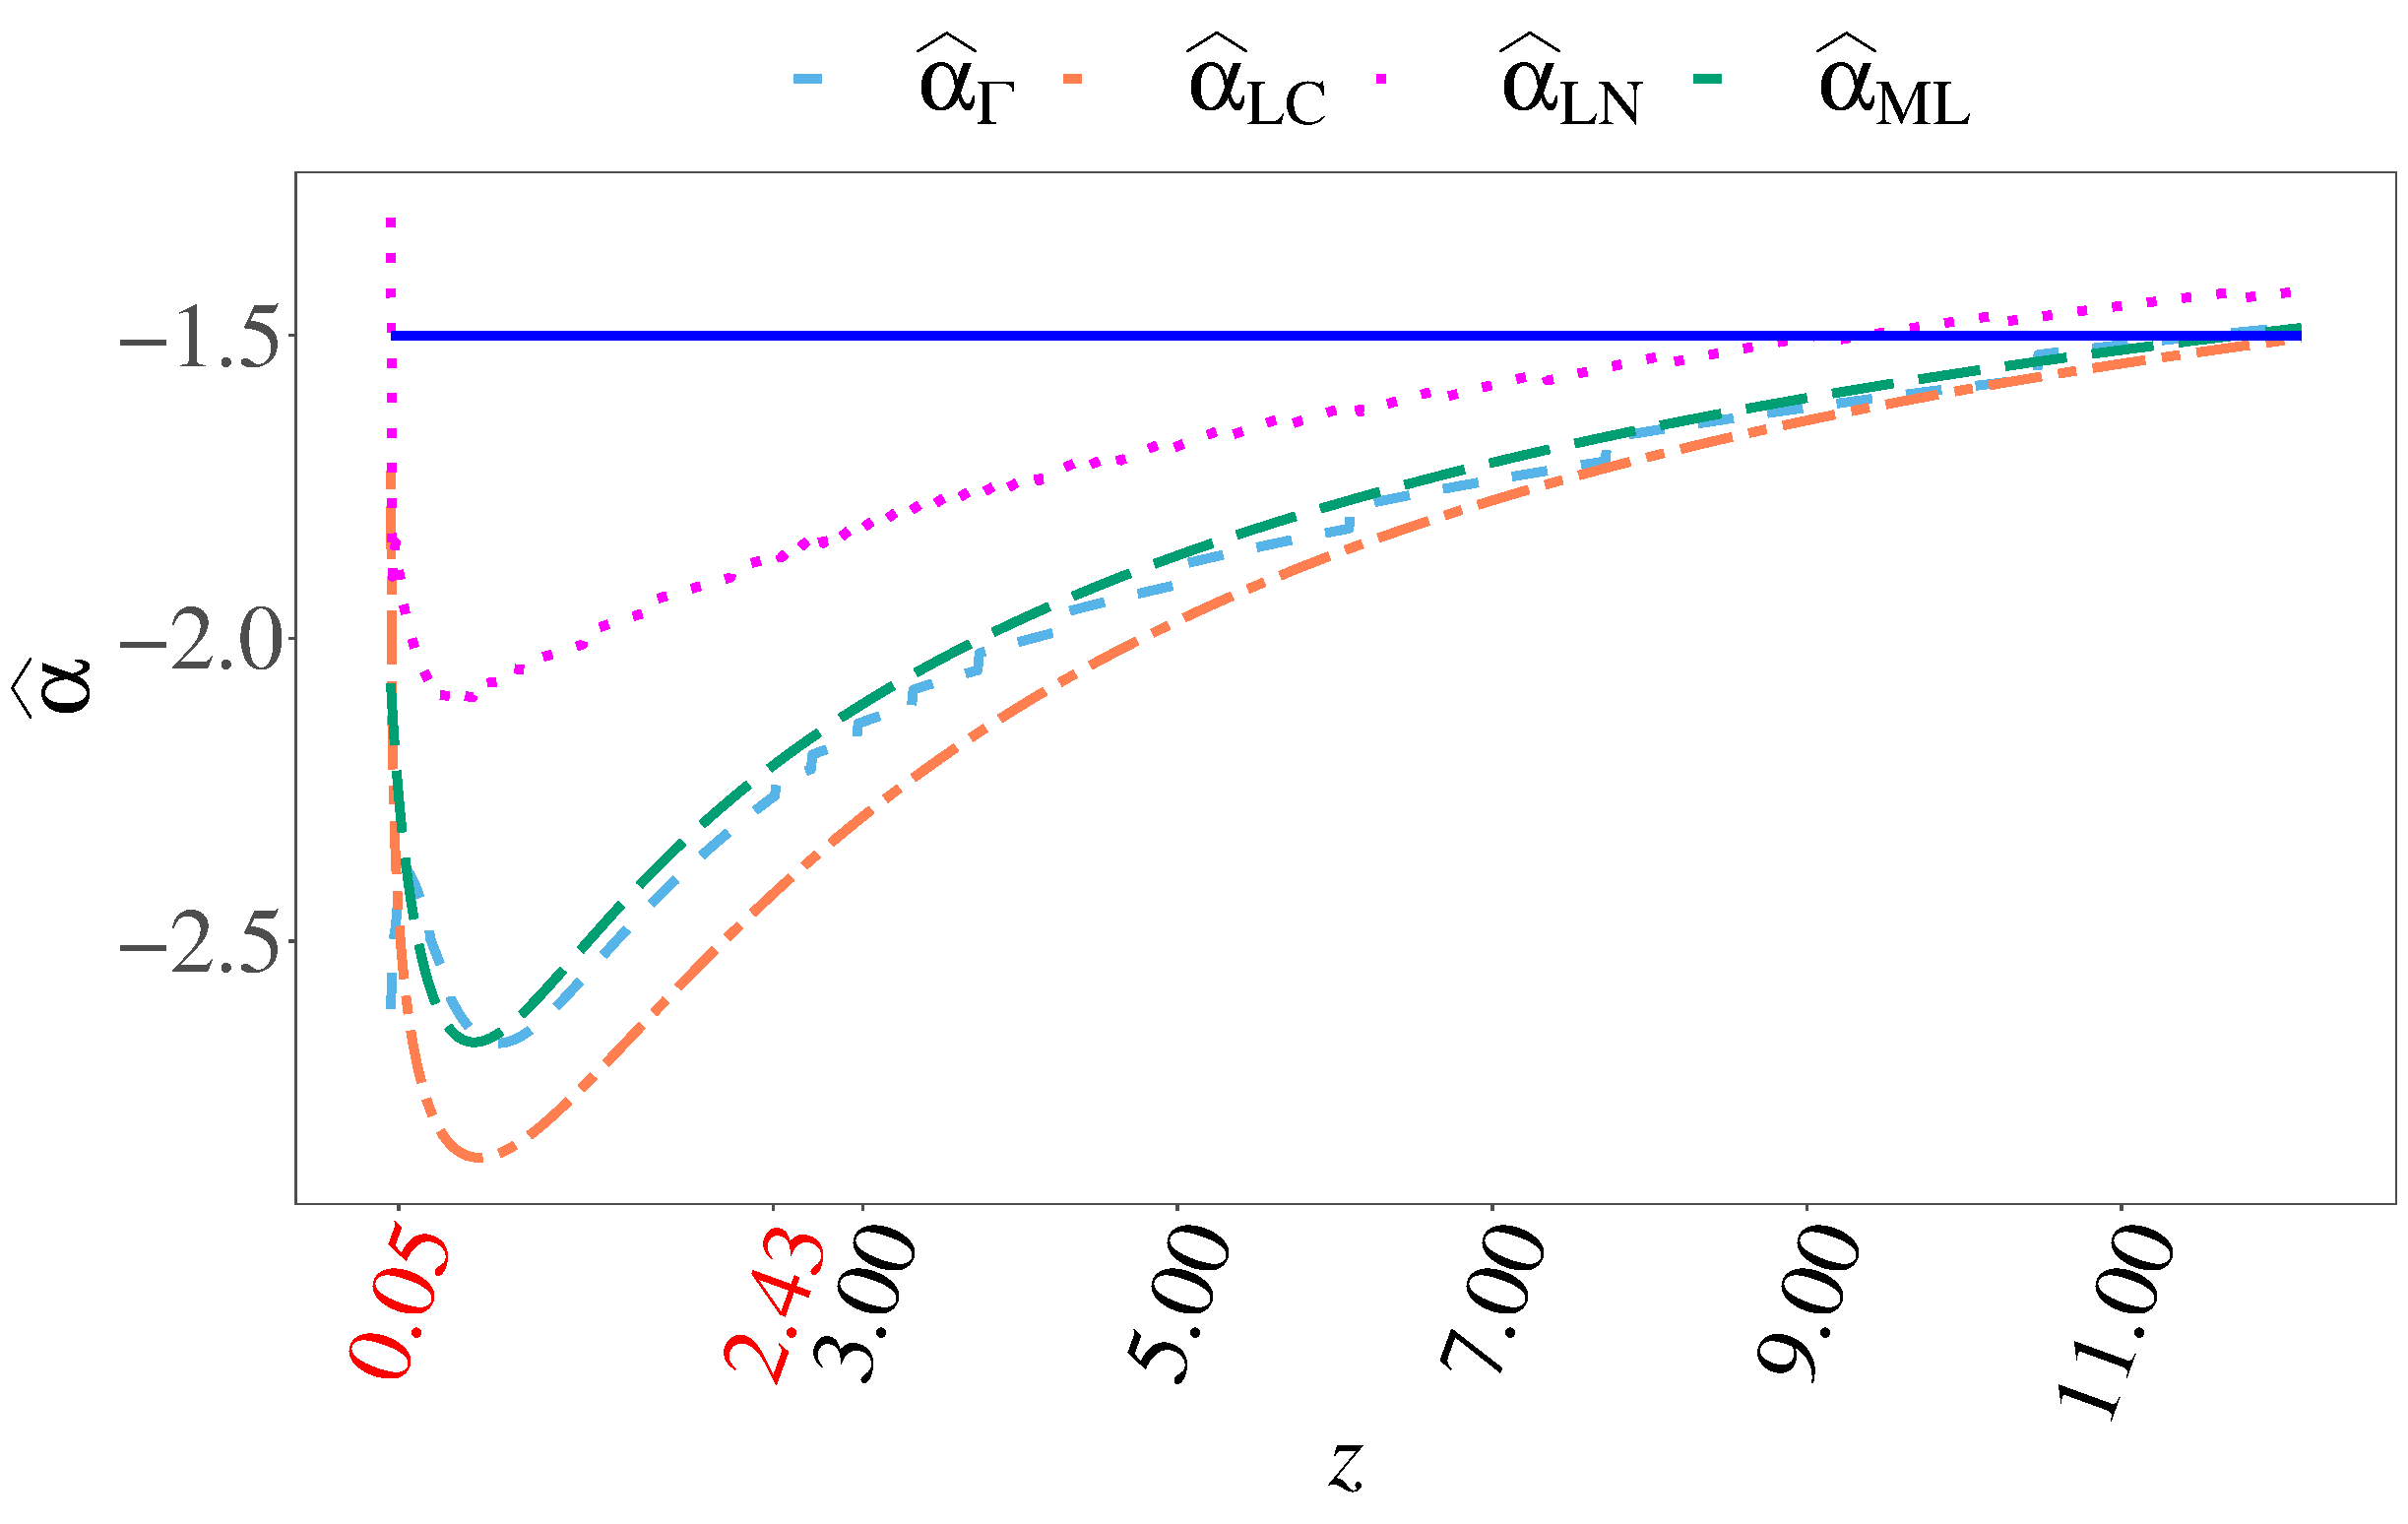
\includegraphics[width=.48\linewidth]{CurvaInfluenciaAlfa-1punto5L3n25}}%JC Programa: GraficoInvluenciaL3alfa-1punto5n25.R
\subfigure[\label{InflL3alfa-3n25}$\widehat{\alpha}=-3$]{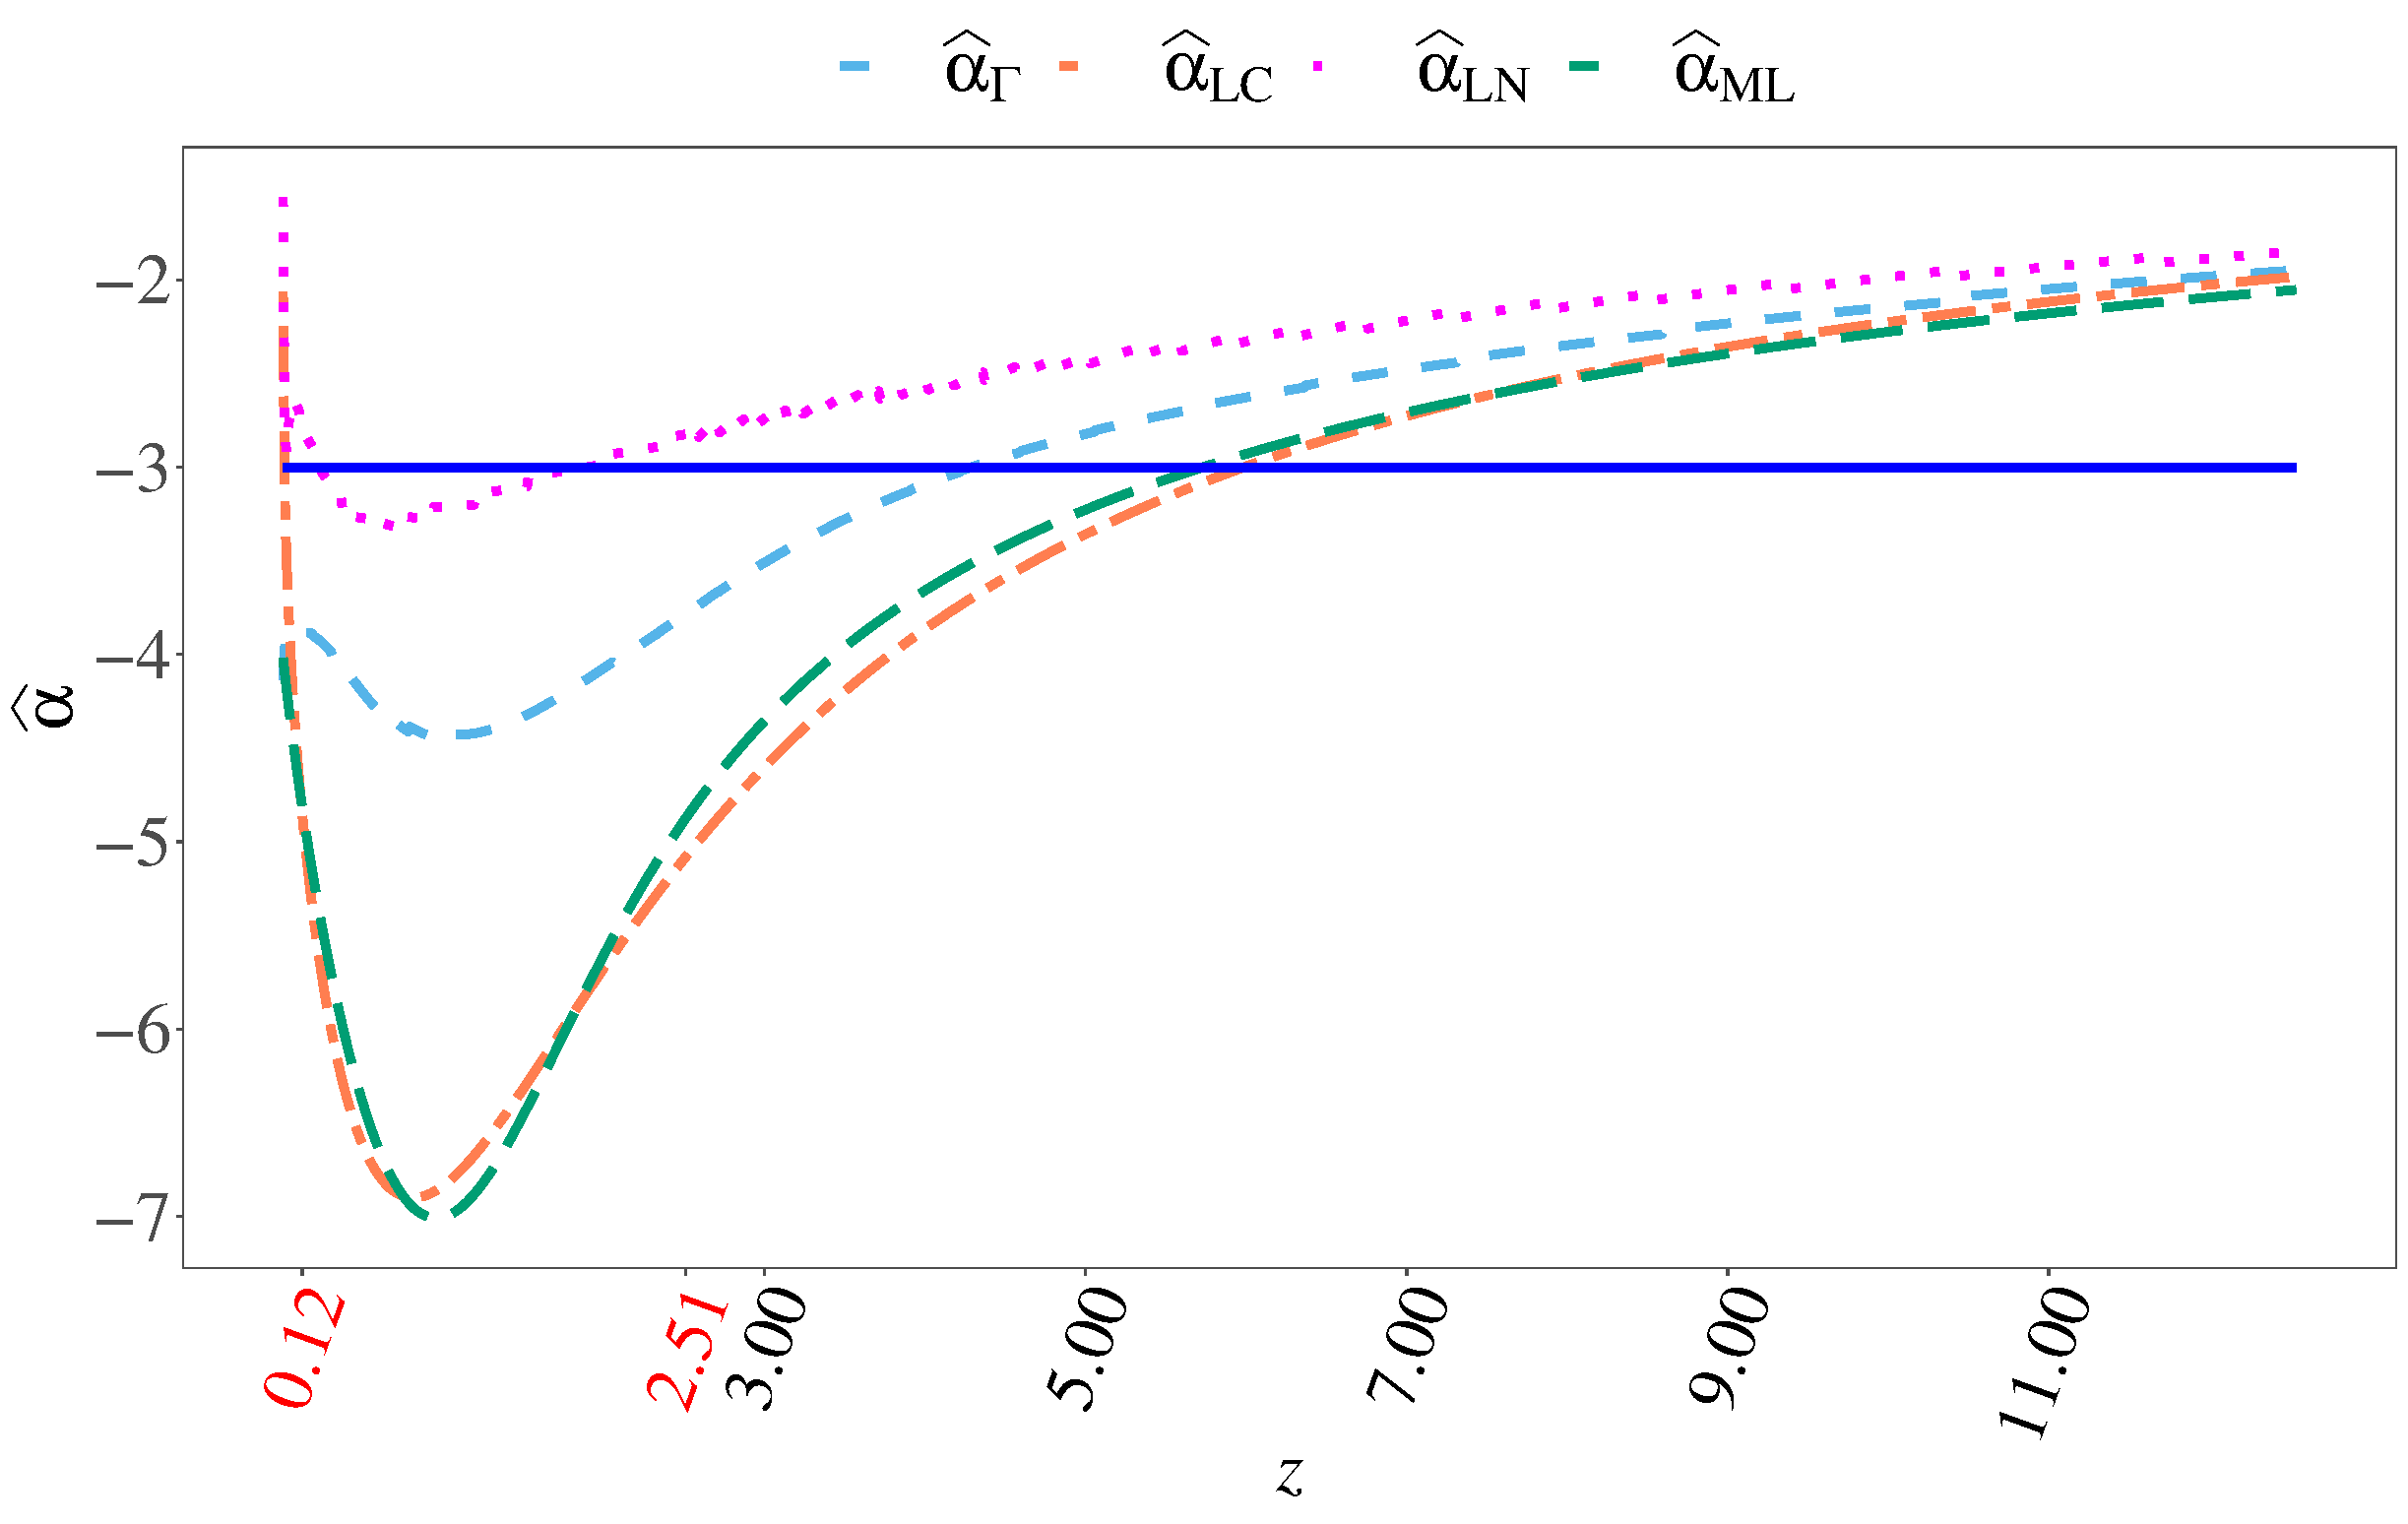
\includegraphics[width=.48\linewidth]{CurvaInfluenciaAlfa-3L3n25}}%JC Programa:GraficoInvluenciaL3alfa-3n25.R
\caption{SEIF for $\widehat{\alpha}_{\text{{ML}}}$, $\widehat{\alpha}_{\Gamma}$, $\widehat{\alpha}_{\text{{LN}}}$, $\widehat{\alpha}_{\text{{{LC}}}}$ para $L=3$, $n=25$ y $\alpha=-1.5,-3$.}\label{SEIFL3a} 
\end{figure}
%JC Programa GraficoInvluenciaL3alfa-1punto5n25.R y GraficoInvluenciaL3alfa-3n25.R

\begin{figure}[hbt]
\centering
\subfigure[\label{InflL3alfa-5n25}$\widehat{\alpha}=-5$]{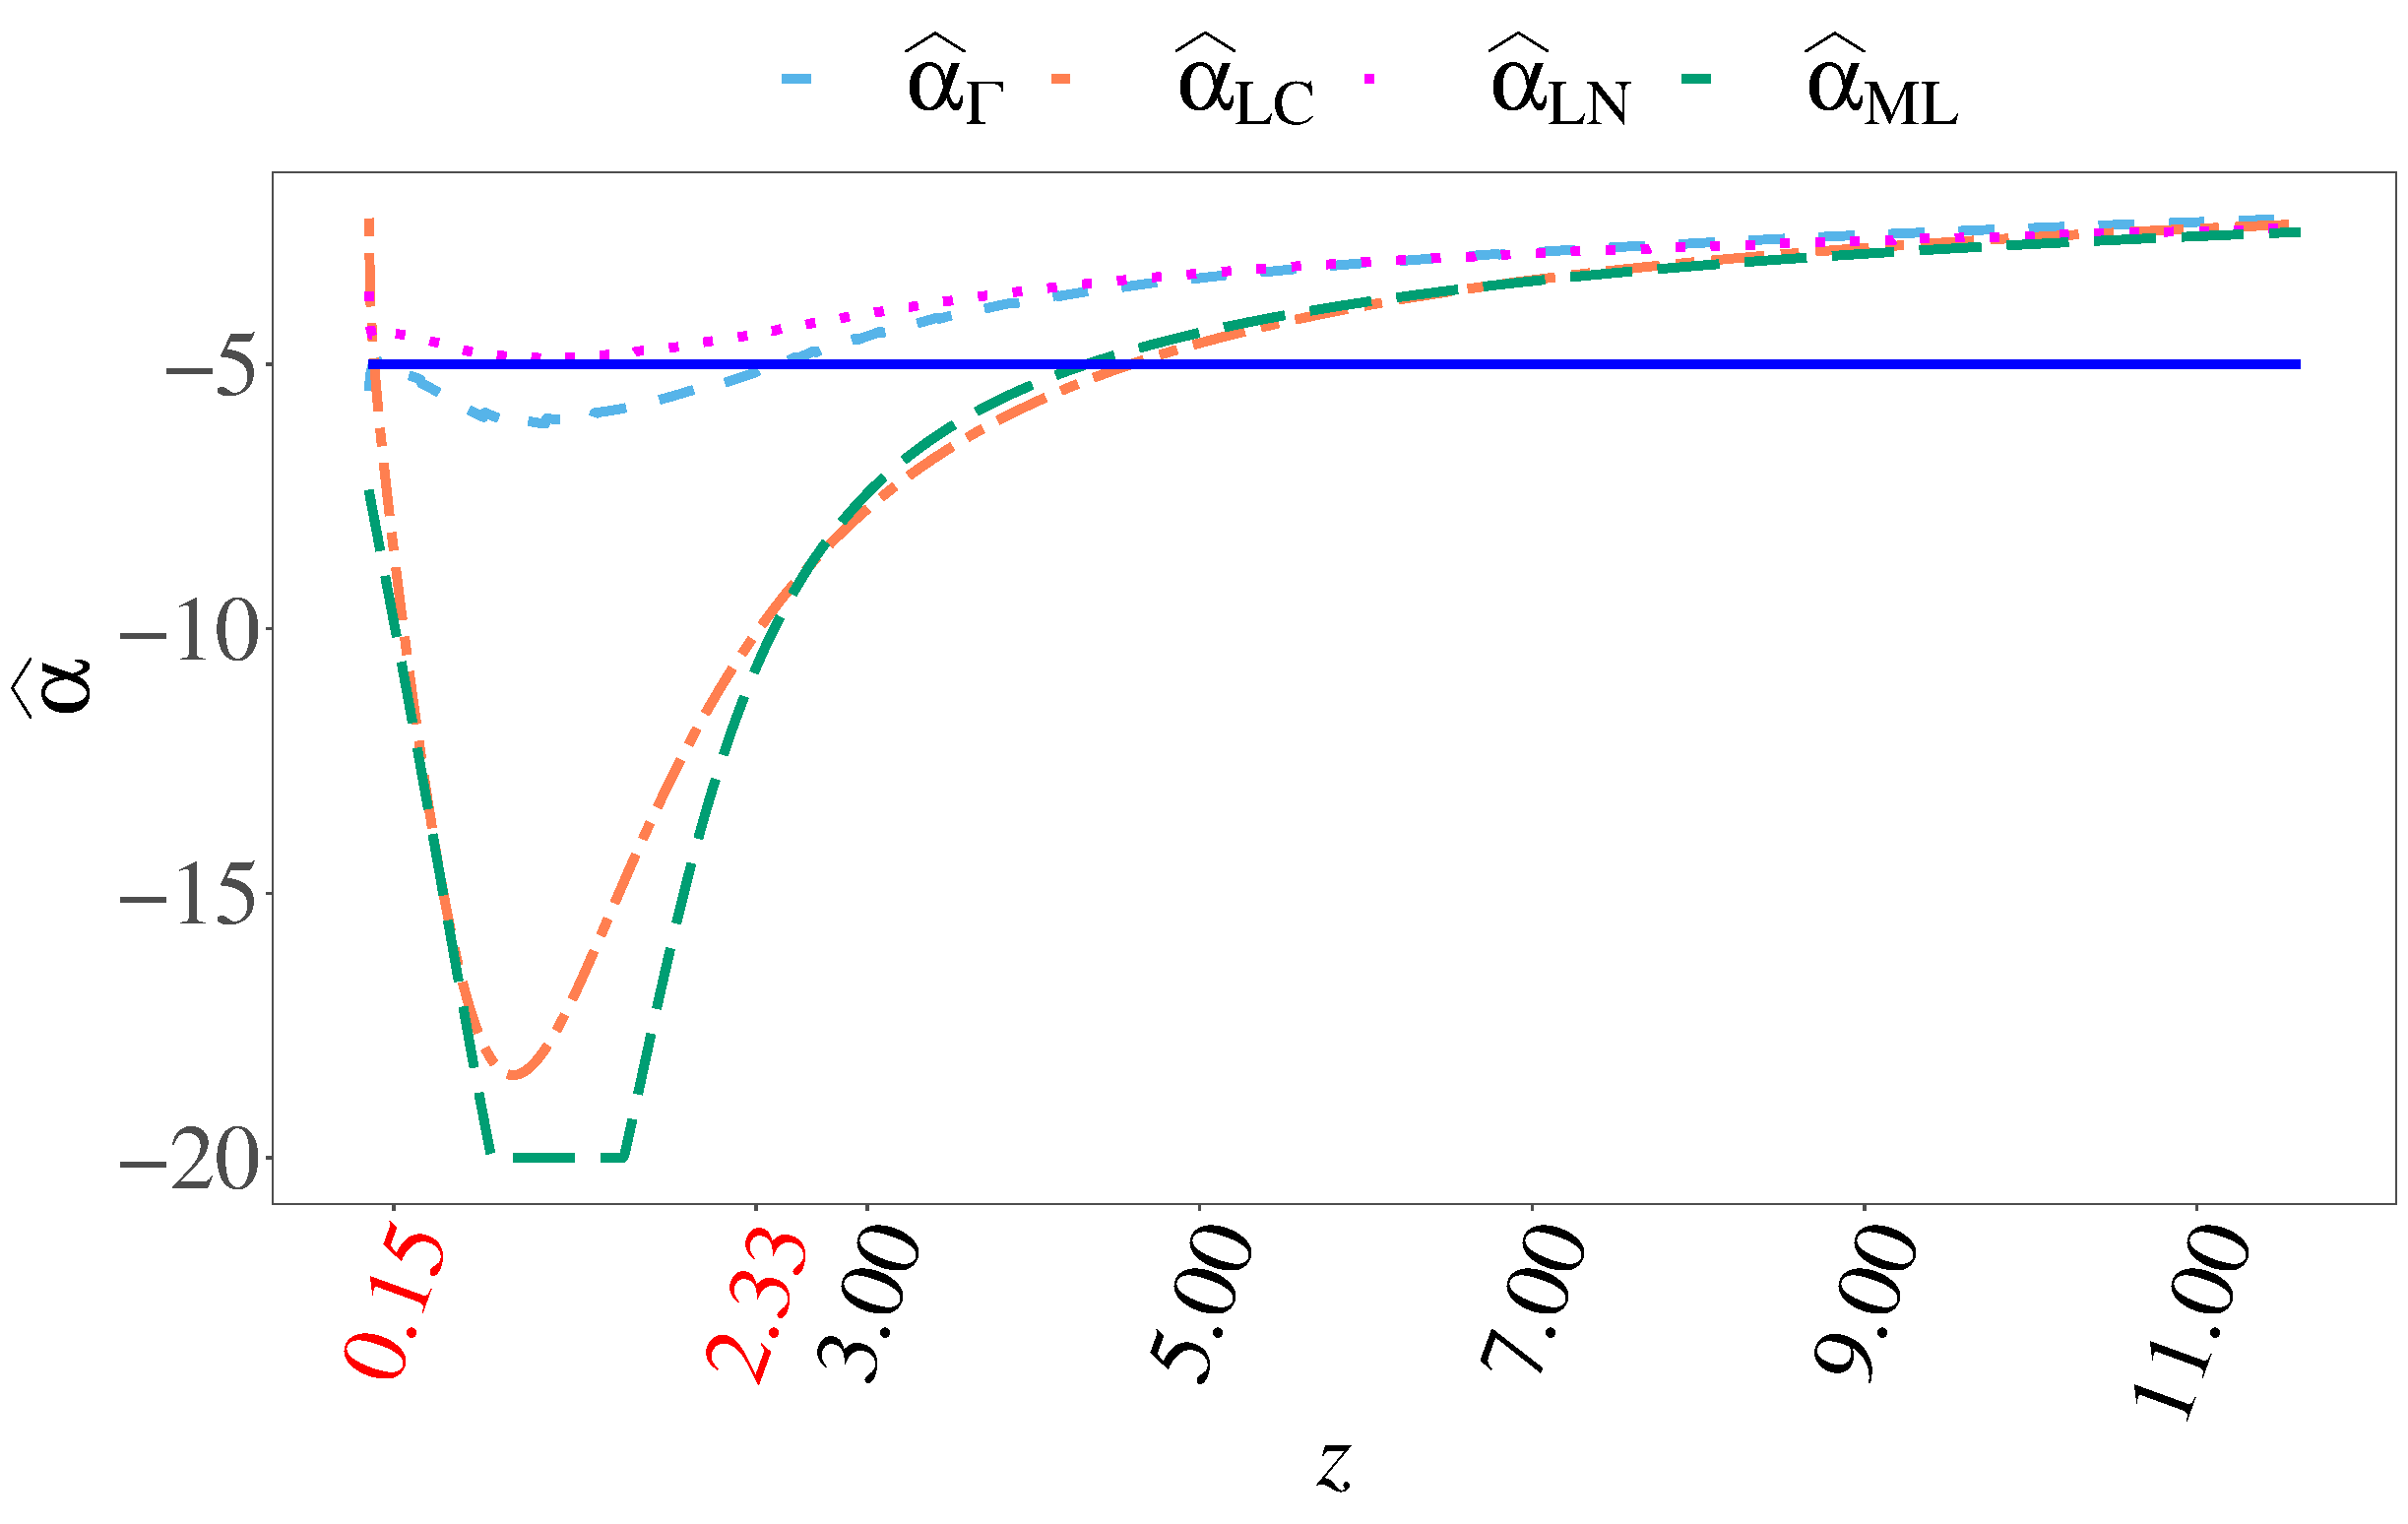
\includegraphics[width=.48\linewidth]{CurvaInfluenciaAlfa-5L3n25}}%JC Programa:GraficoInvluenciaL3alfa-5n25.R
\subfigure[\label{InflL3alfa-8n25}$\widehat{\alpha}=-8$]{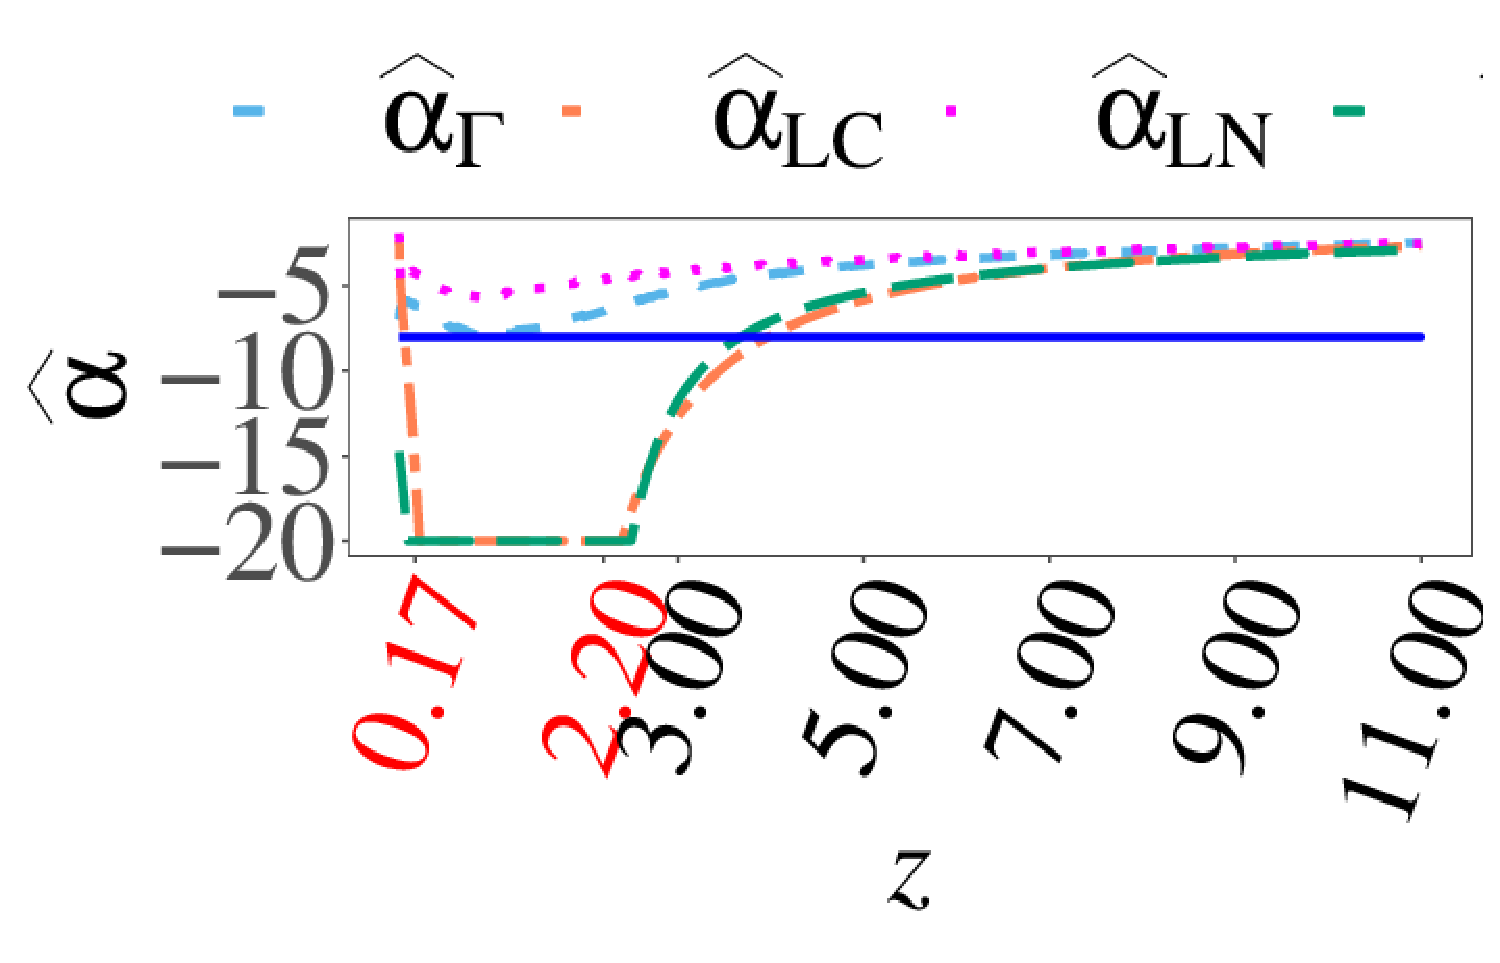
\includegraphics[width=.48\linewidth]{CurvaInfluenciaAlfa-8L3n25}}%JC Programa:GraficoInvluenciaL3alfa-8n25.R
\caption{SEIF for $\widehat{\alpha}_{\text{{ML}}}$, $\widehat{\alpha}_{\Gamma}$, $\widehat{\alpha}_{\text{{LN}}}$, $\widehat{\alpha}_{\text{{{LC}}}}$ para $L=3$, $n=25$ y $\alpha=-5,-8$.}\label{SEIFL3b} 
\end{figure}
%JC Programa GraficoInvluenciaL3alfa-5n25.R y GraficoInvluenciaL3alfa-8n25.R

\begin{figure}[hbt]
\centering
\subfigure[\label{InflL8alfa-1.5n25}$\widehat{\alpha}=-1.5$]{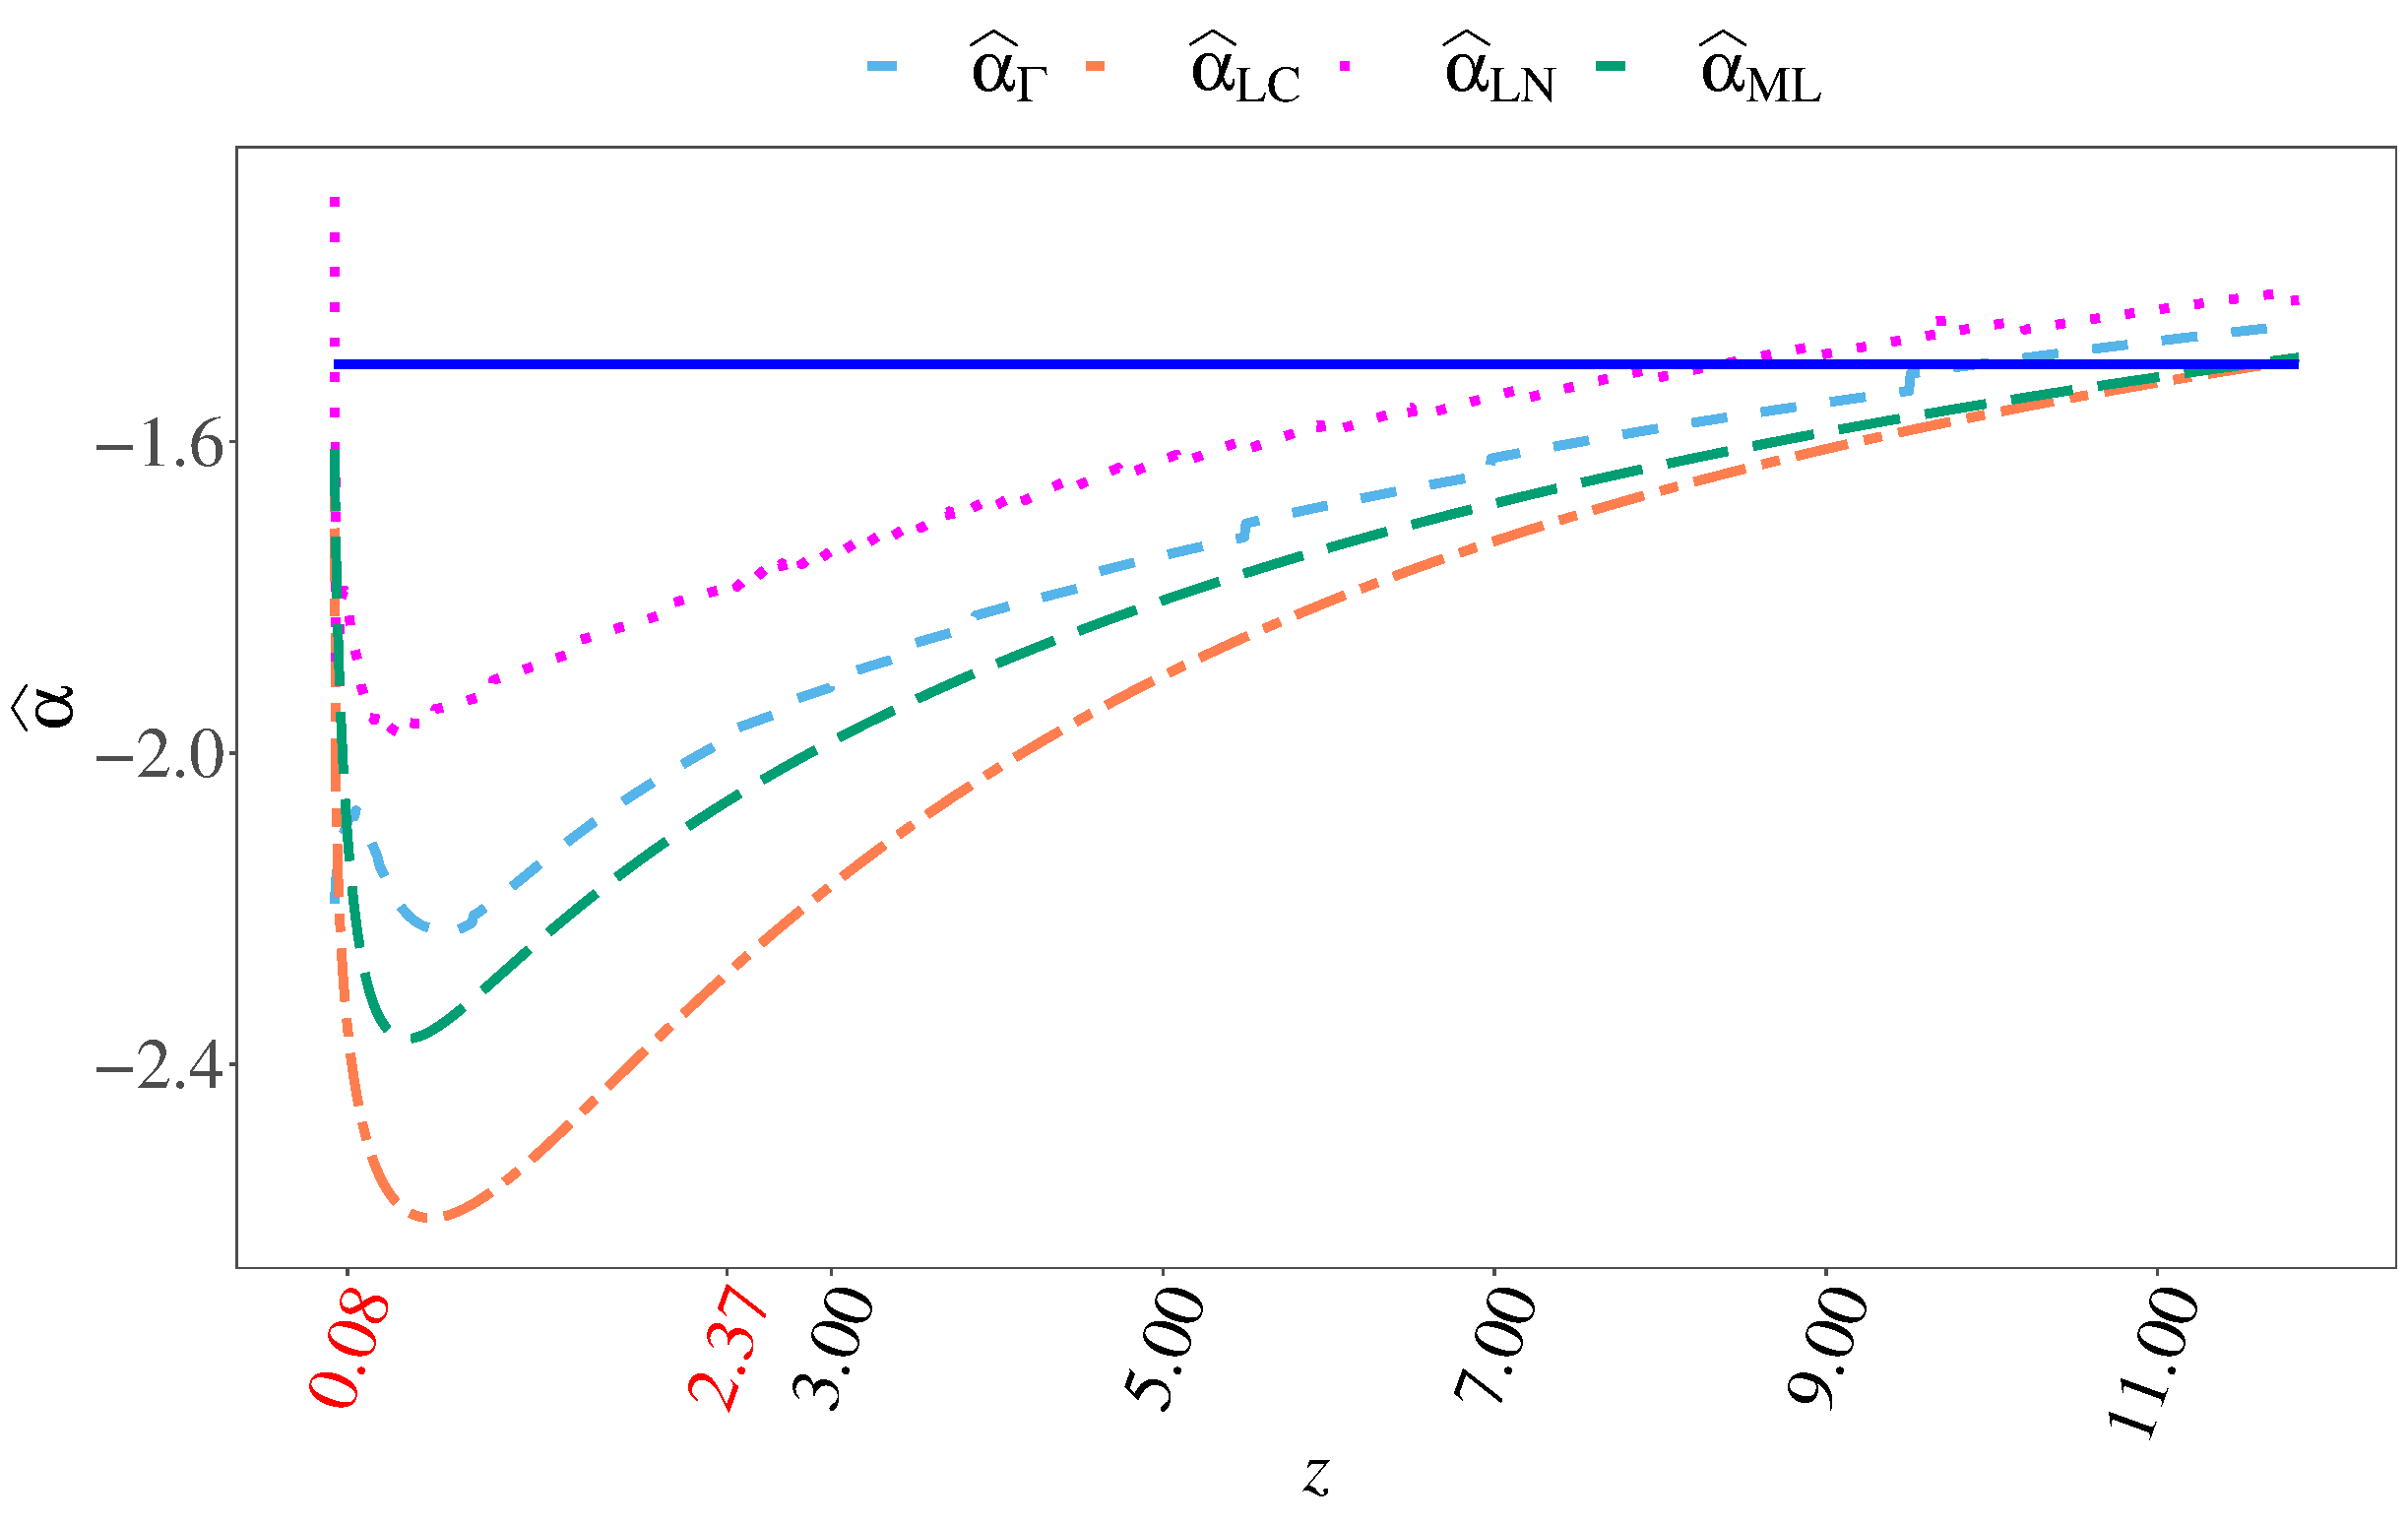
\includegraphics[width=.48\linewidth]{CurvaInfluenciaAlfa-1punto5L8n25}}%JC Programa: GraficoInvluenciaL8alfa-1punto5n25.R
\subfigure[\label{InflL8alfa-3n25}$\widehat{\alpha}=-3$]{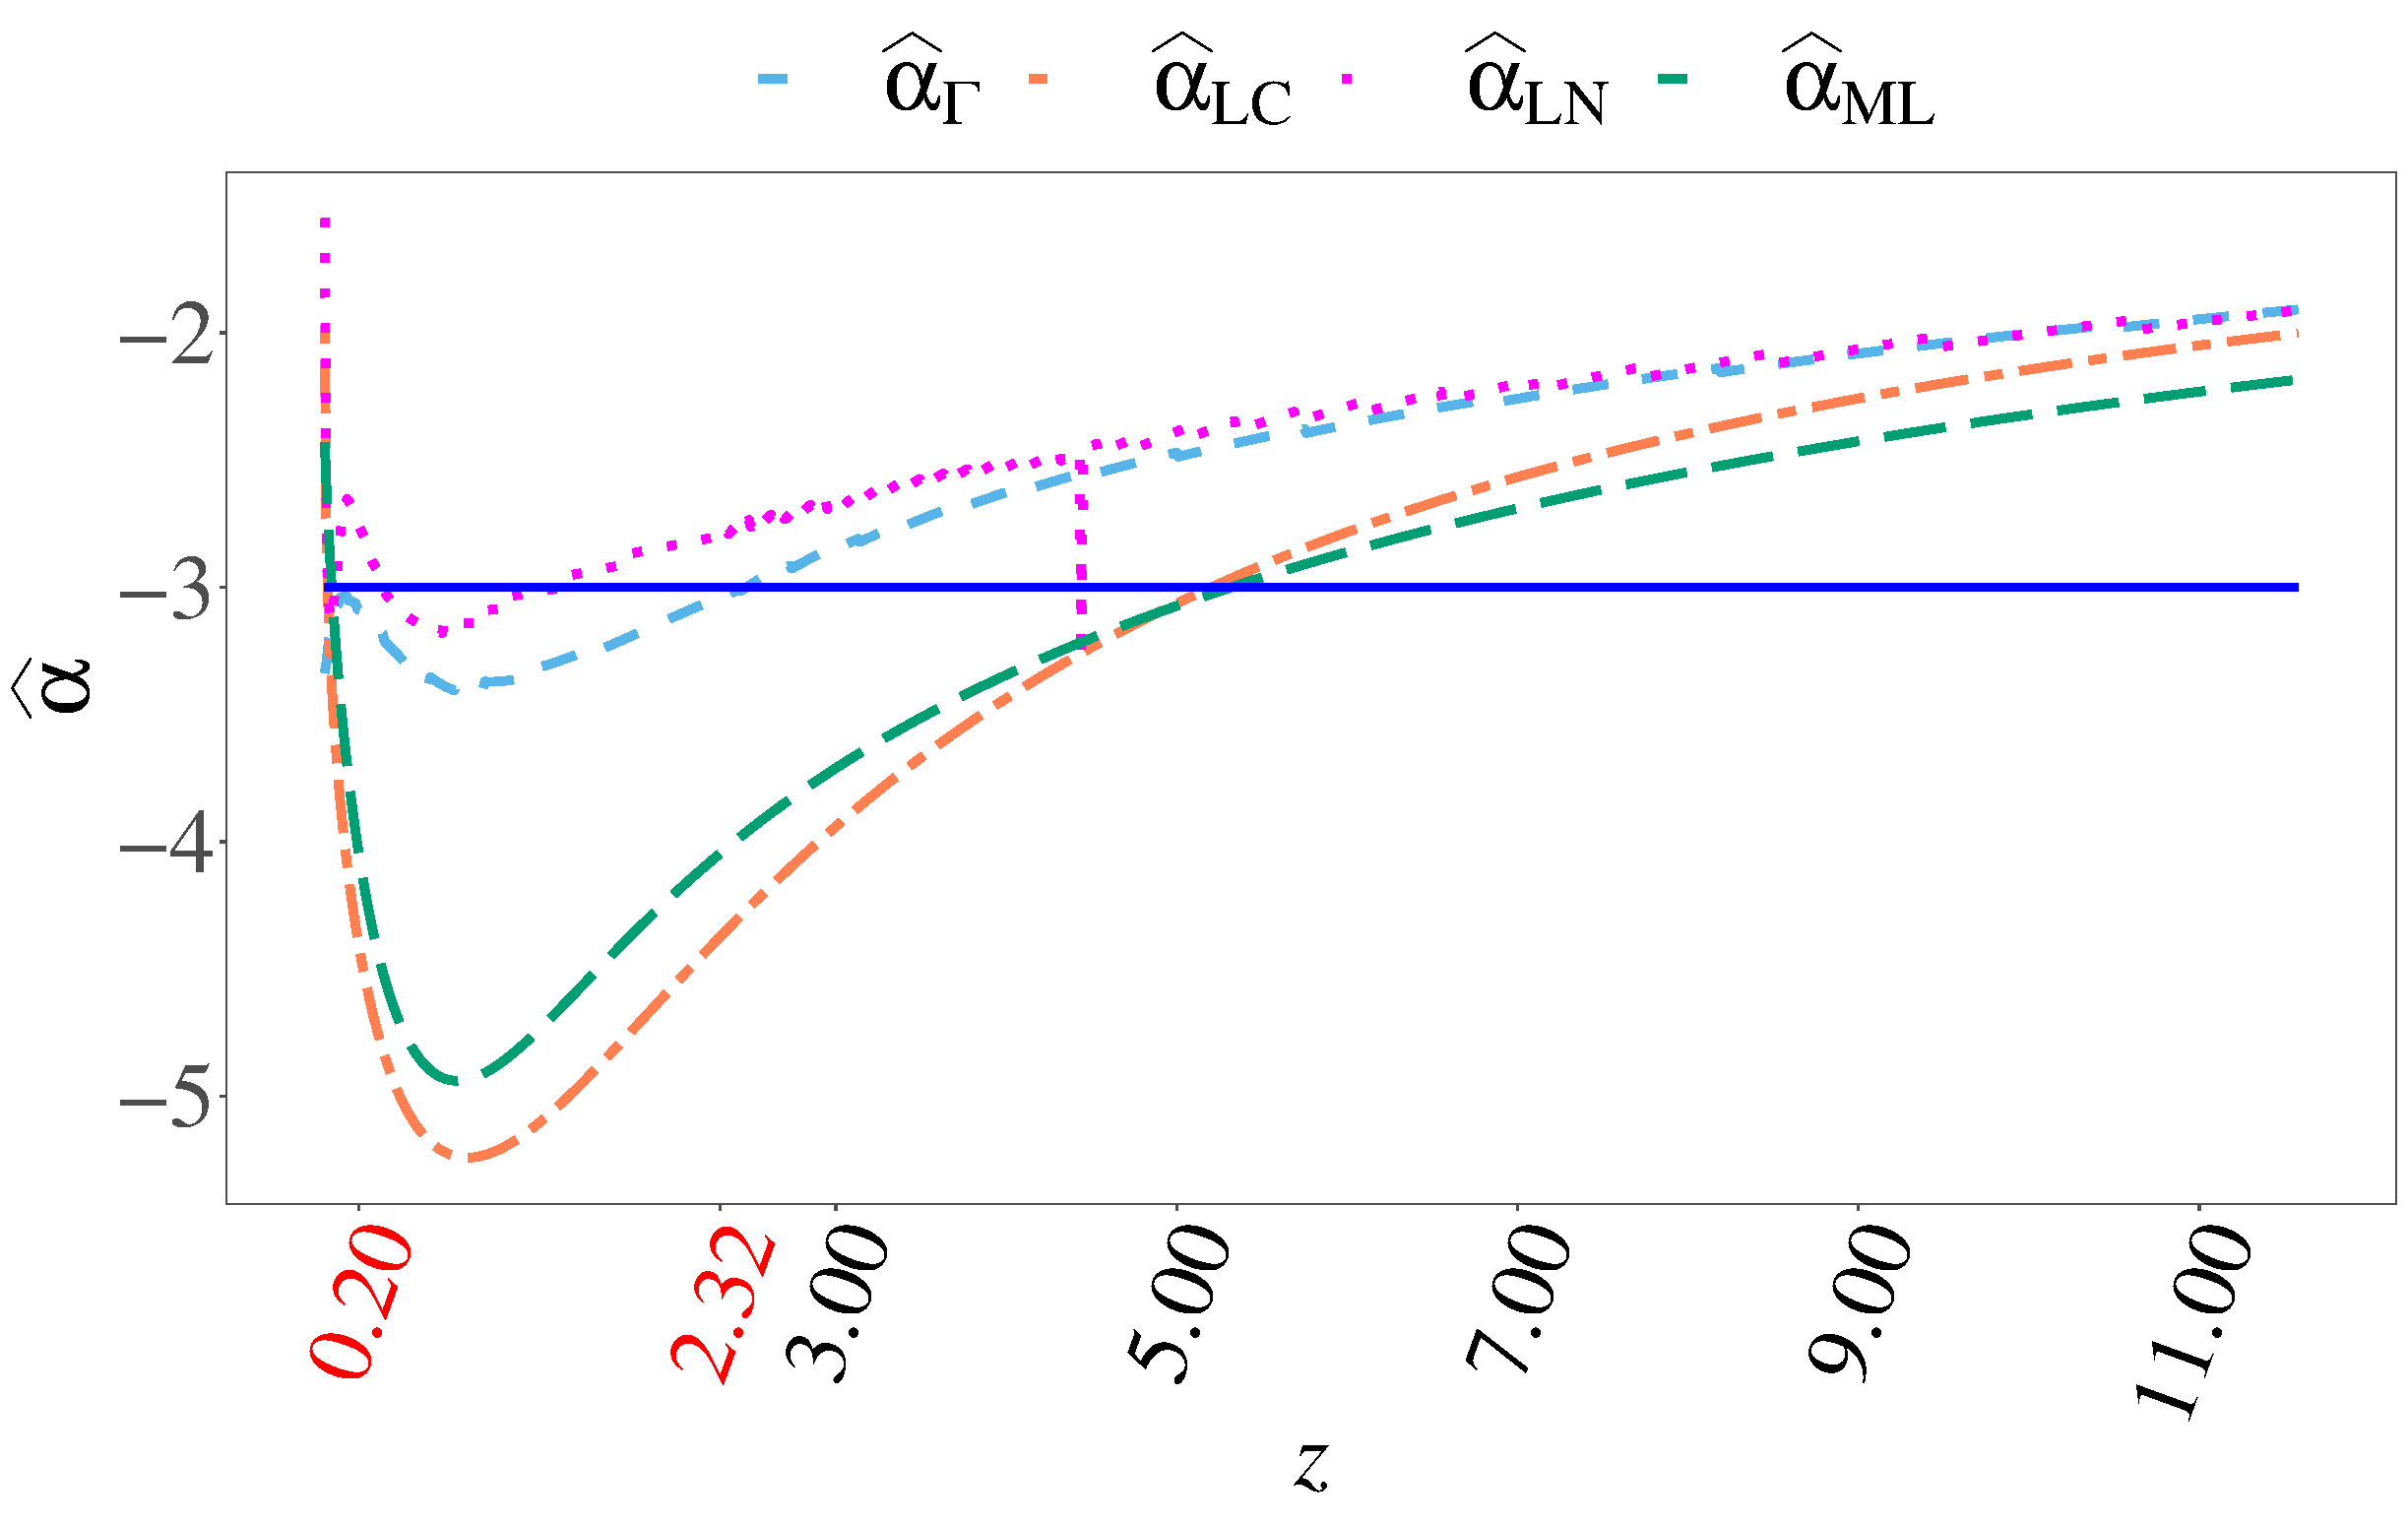
\includegraphics[width=.48\linewidth]{CurvaInfluenciaAlfa-3L8n25}}%JC Programa: GraficoInvluenciaL8alfa-3n25.R
\caption{SEIF for $\widehat{\alpha}_{\text{{ML}}}$, $\widehat{\alpha}_{\Gamma}$, $\widehat{\alpha}_{\text{{LN}}}$, $\widehat{\alpha}_{\text{{{LC}}}}$ para $L=8$, $n=25$ y $\alpha=-1.5,-3$.}\label{SEIFL8a} 
\end{figure}
%JC Programa GraficoInvluenciaL8alfa-1punto5n25.R y GraficoInvluenciaL3alfa-3n25.R


\begin{figure}[hbt]
\centering
\subfigure[\label{InflL8alfa-5n25}$\widehat{\alpha}=-5$]{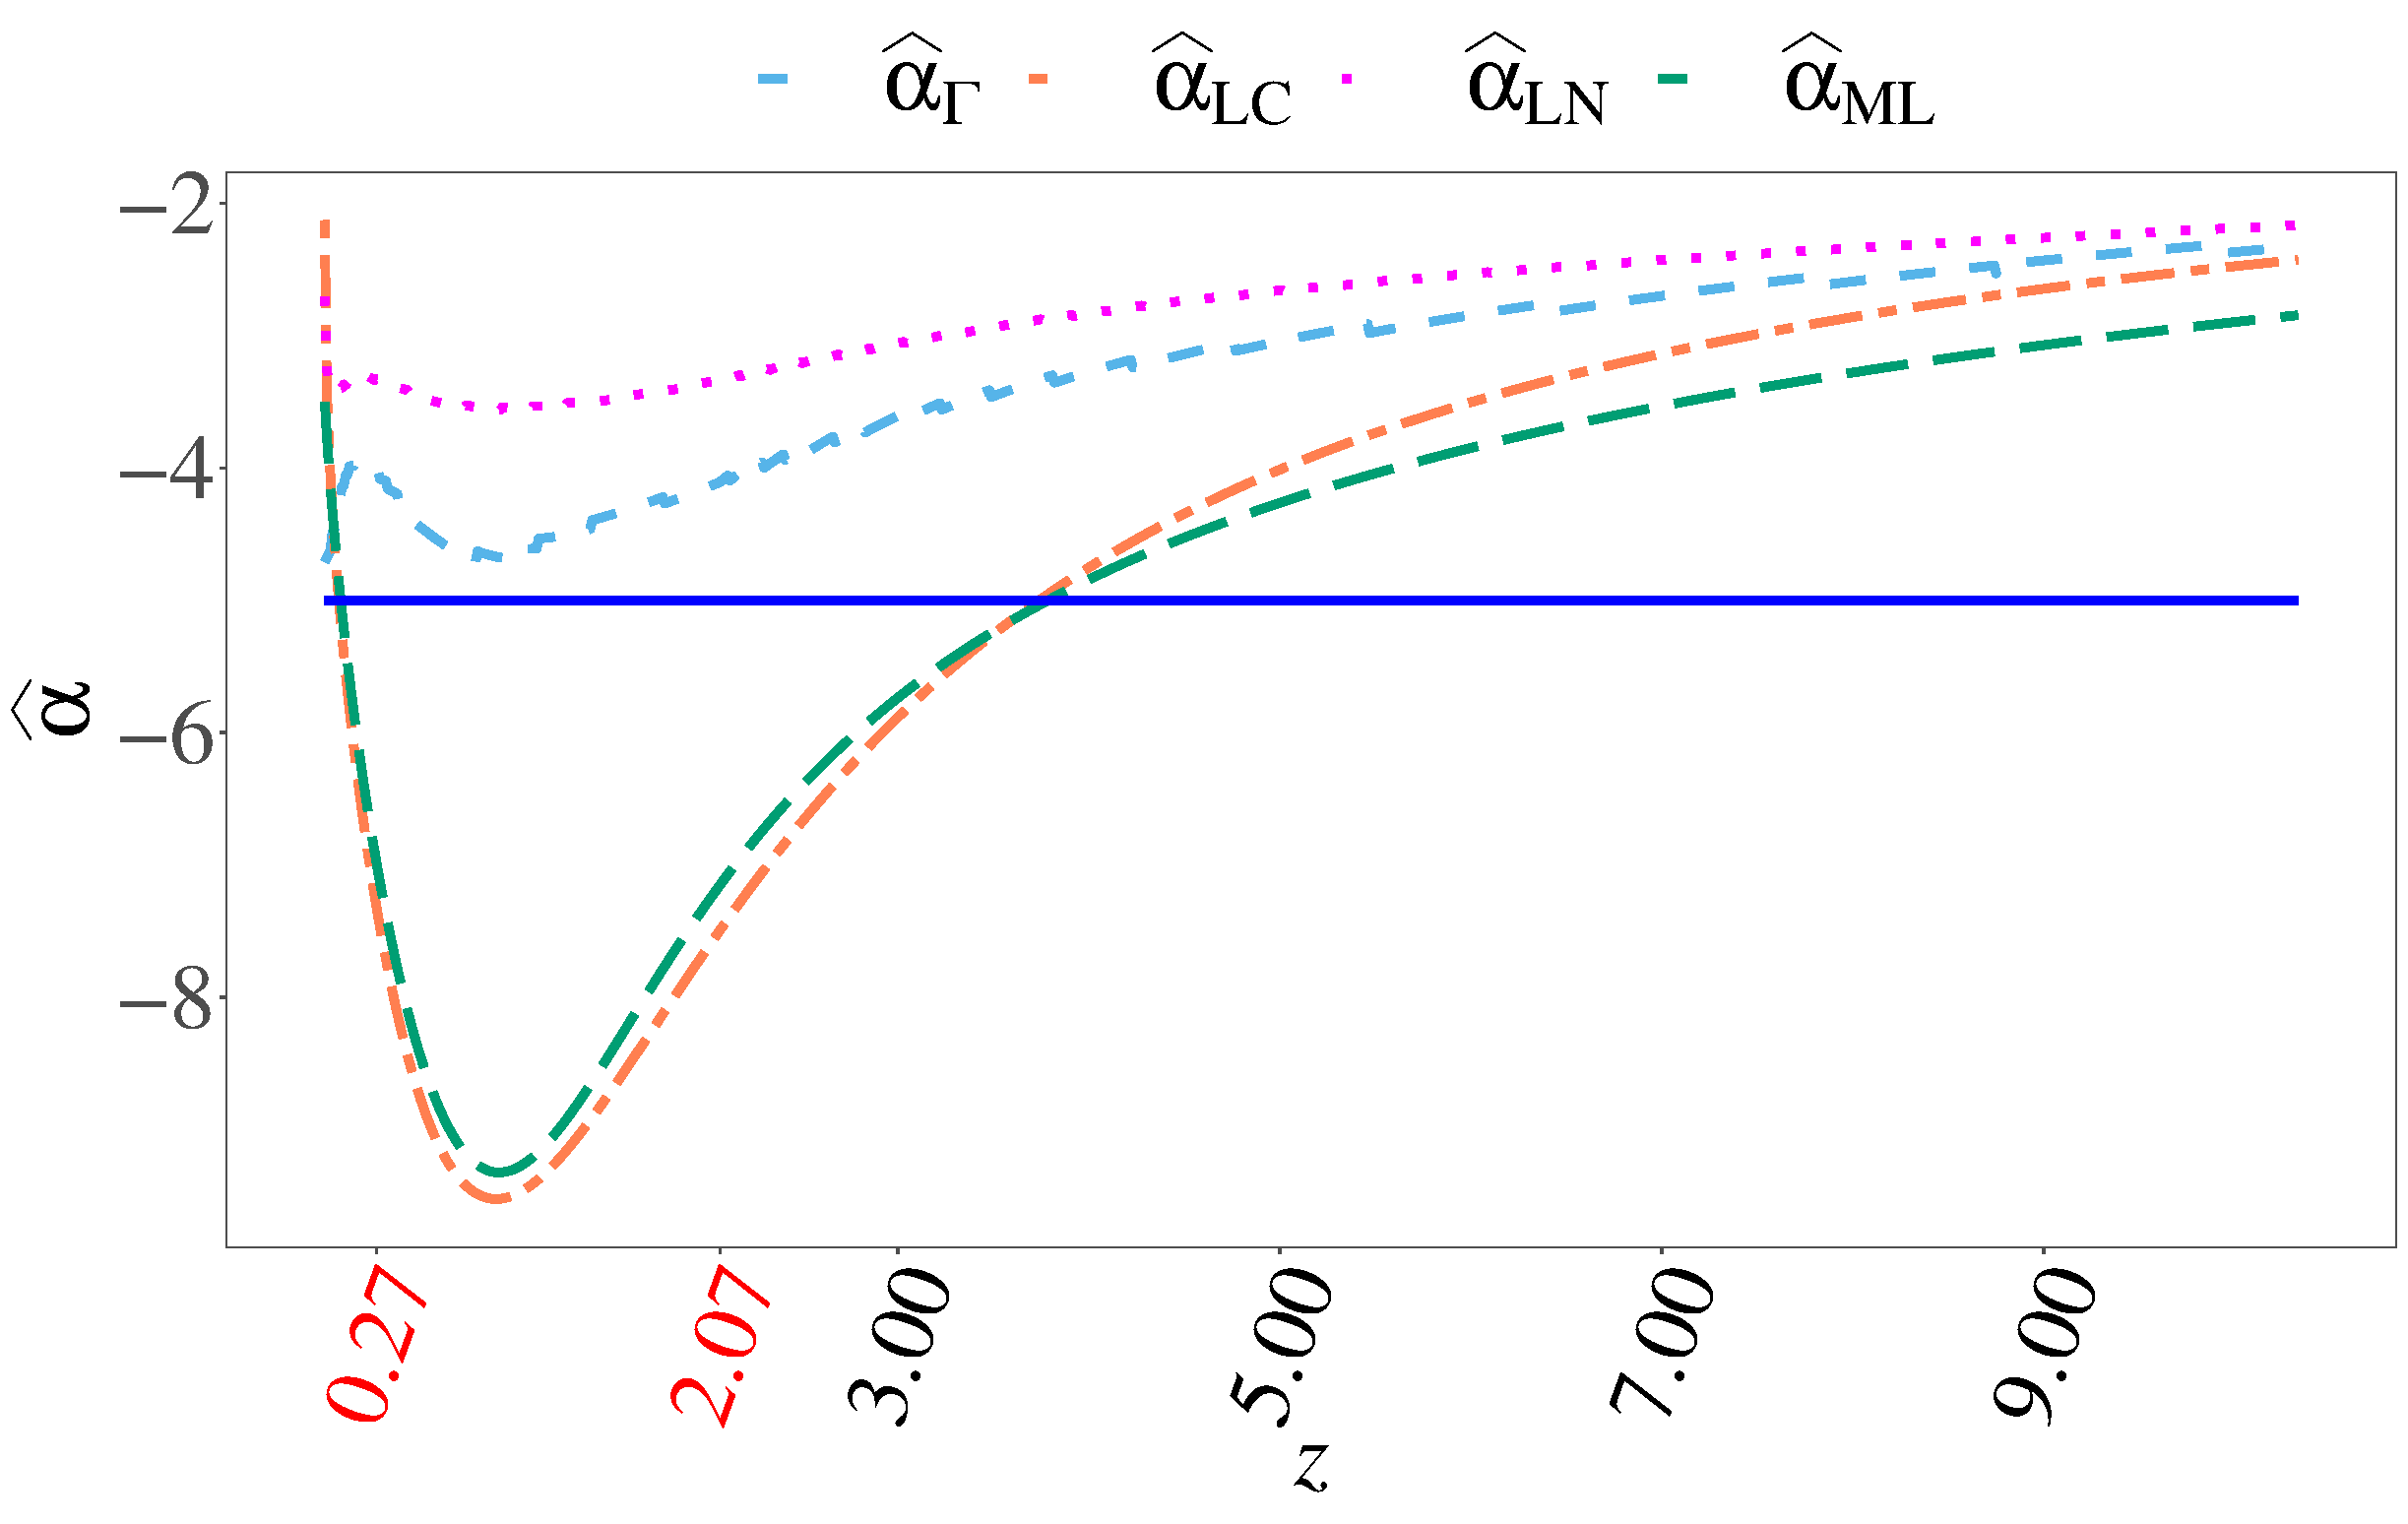
\includegraphics[width=.48\linewidth]{CurvaInfluenciaAlfa-5L8n25}}%JC Programa: GraficoInvluenciaL8alfa-5n25.R
\subfigure[\label{InflL8alfa-8n25}$\widehat{\alpha}=-8$]{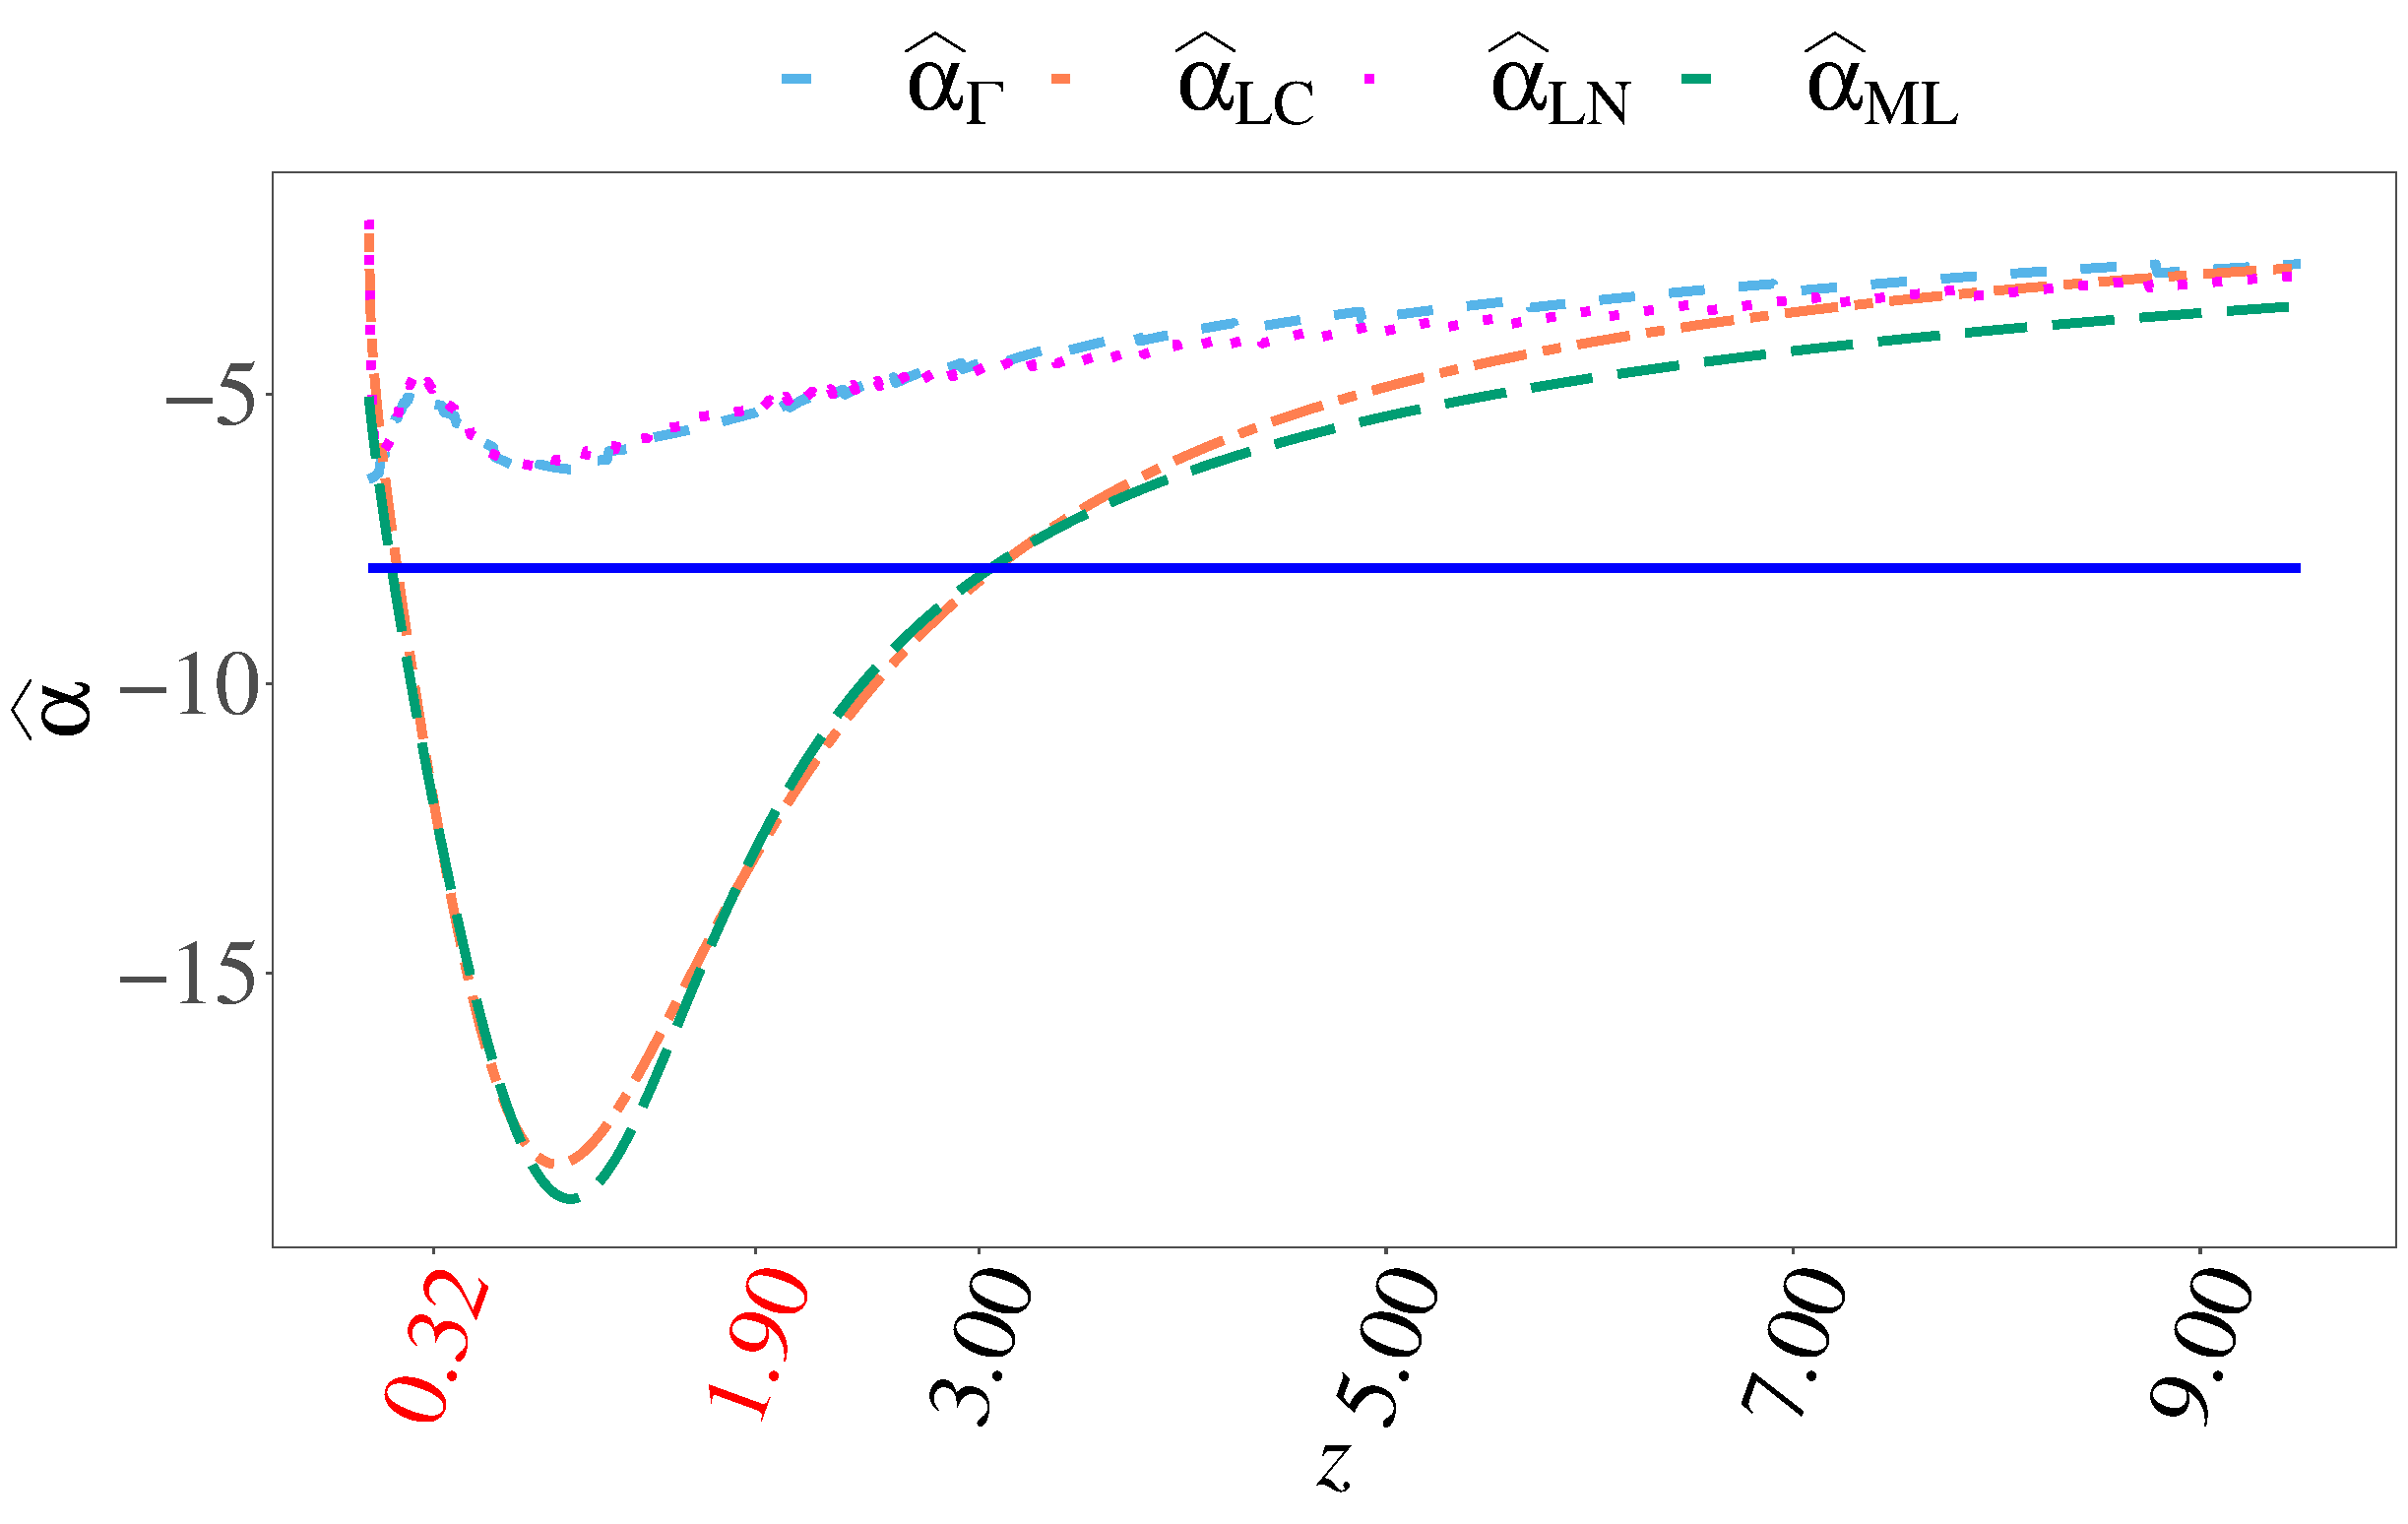
\includegraphics[width=.48\linewidth]{CurvaInfluenciaAlfa-8L8n25}}%JC Programa: GraficoInvluenciaL8alfa-8n25.R
\caption{SEIF for $\widehat{\alpha}_{\text{{ML}}}$, $\widehat{\alpha}_{\Gamma}$, $\widehat{\alpha}_{\text{{LN}}}$, $\widehat{\alpha}_{\text{{LC}}}$ para $L=8$, $n=25$ y $\alpha=-5,-8$.}\label{SEIFL8b} 
\end{figure}
%JC Programa GraficoInvluenciaL8alfa-5n25.R y GraficoInvluenciaL3alfa-8n25.R

Again, for $\alpha=-3, -5, -8$, we see a similar behavior between $\widehat{\alpha}_{\text{{ML}}}$, $\widehat{\alpha}_{\text{{LC}}}$ on the one hand, and $\widehat{\alpha}_{\Gamma}$ and $\widehat{\alpha}_{\text{{LN}}}$ on the other hand.
In extremely textured areas $\widehat{\alpha}_{\text{{LN}}}$ has the best performance, while for $z$ values lower than the last quantile and for the rest of the textures, both $\widehat{\alpha}_{\Gamma}$ and $\widehat{\alpha}_{\text{{LN}}}$ have a better performance compared to the other estimators. 
Moreover, $\widehat{\alpha}_{\text{{ML}}}$ does not converge for moderately heterogeneous and homogeneous zones, while $\widehat{\alpha}_{\text{{LC}}}$ does not converge for homogeneous zones. All estimators behave similarly for large values of $z$. 
This behavior shows the sensitivity and loss of robustness for $\widehat{\alpha}_{\text{{ML}}}$ and $\widehat{\alpha}_{\text{{LC}}}$ versus MDEs.

Figures~\ref{InflL8alfa-1.5n25}, \ref{InflL8alfa-3n25}, \ref{InflL8alfa-5n25} and~\ref{InflL8alfa-8n25} show the SEIFS for $L=8$ and the same values of $n$ and $\alpha$. 
The performance of the estimators for this case is similar to that described for $L=3$. 
It should be mentioned that all methods converge for this case where there is less presence of speckle noise.

%%%%%%%%%%%%%%%%%%%%%%%%%%%%%%%%%¨

\subsection{Simulation Results -- Contamination Data}
\label{CasesCont}

In the following, we show the performance, throughout the bias and mean square error, of the estimators under contamination. 
Figures~\ref{SesgoyECMConContL=3} and~\ref{SesgoyECMConContL=8} present these quantities under contaminated data for $L=3$ and $L=8$ respectively. In this case we considered $\epsilon=0.05$

%%%%%%%%%%%%%%%%%% EPSILON 0.05
\begin{figure*}[hbt]
\centering
\subfigure[\label{SesgoConContL=3}$\widehat{\text{Bias}}$]{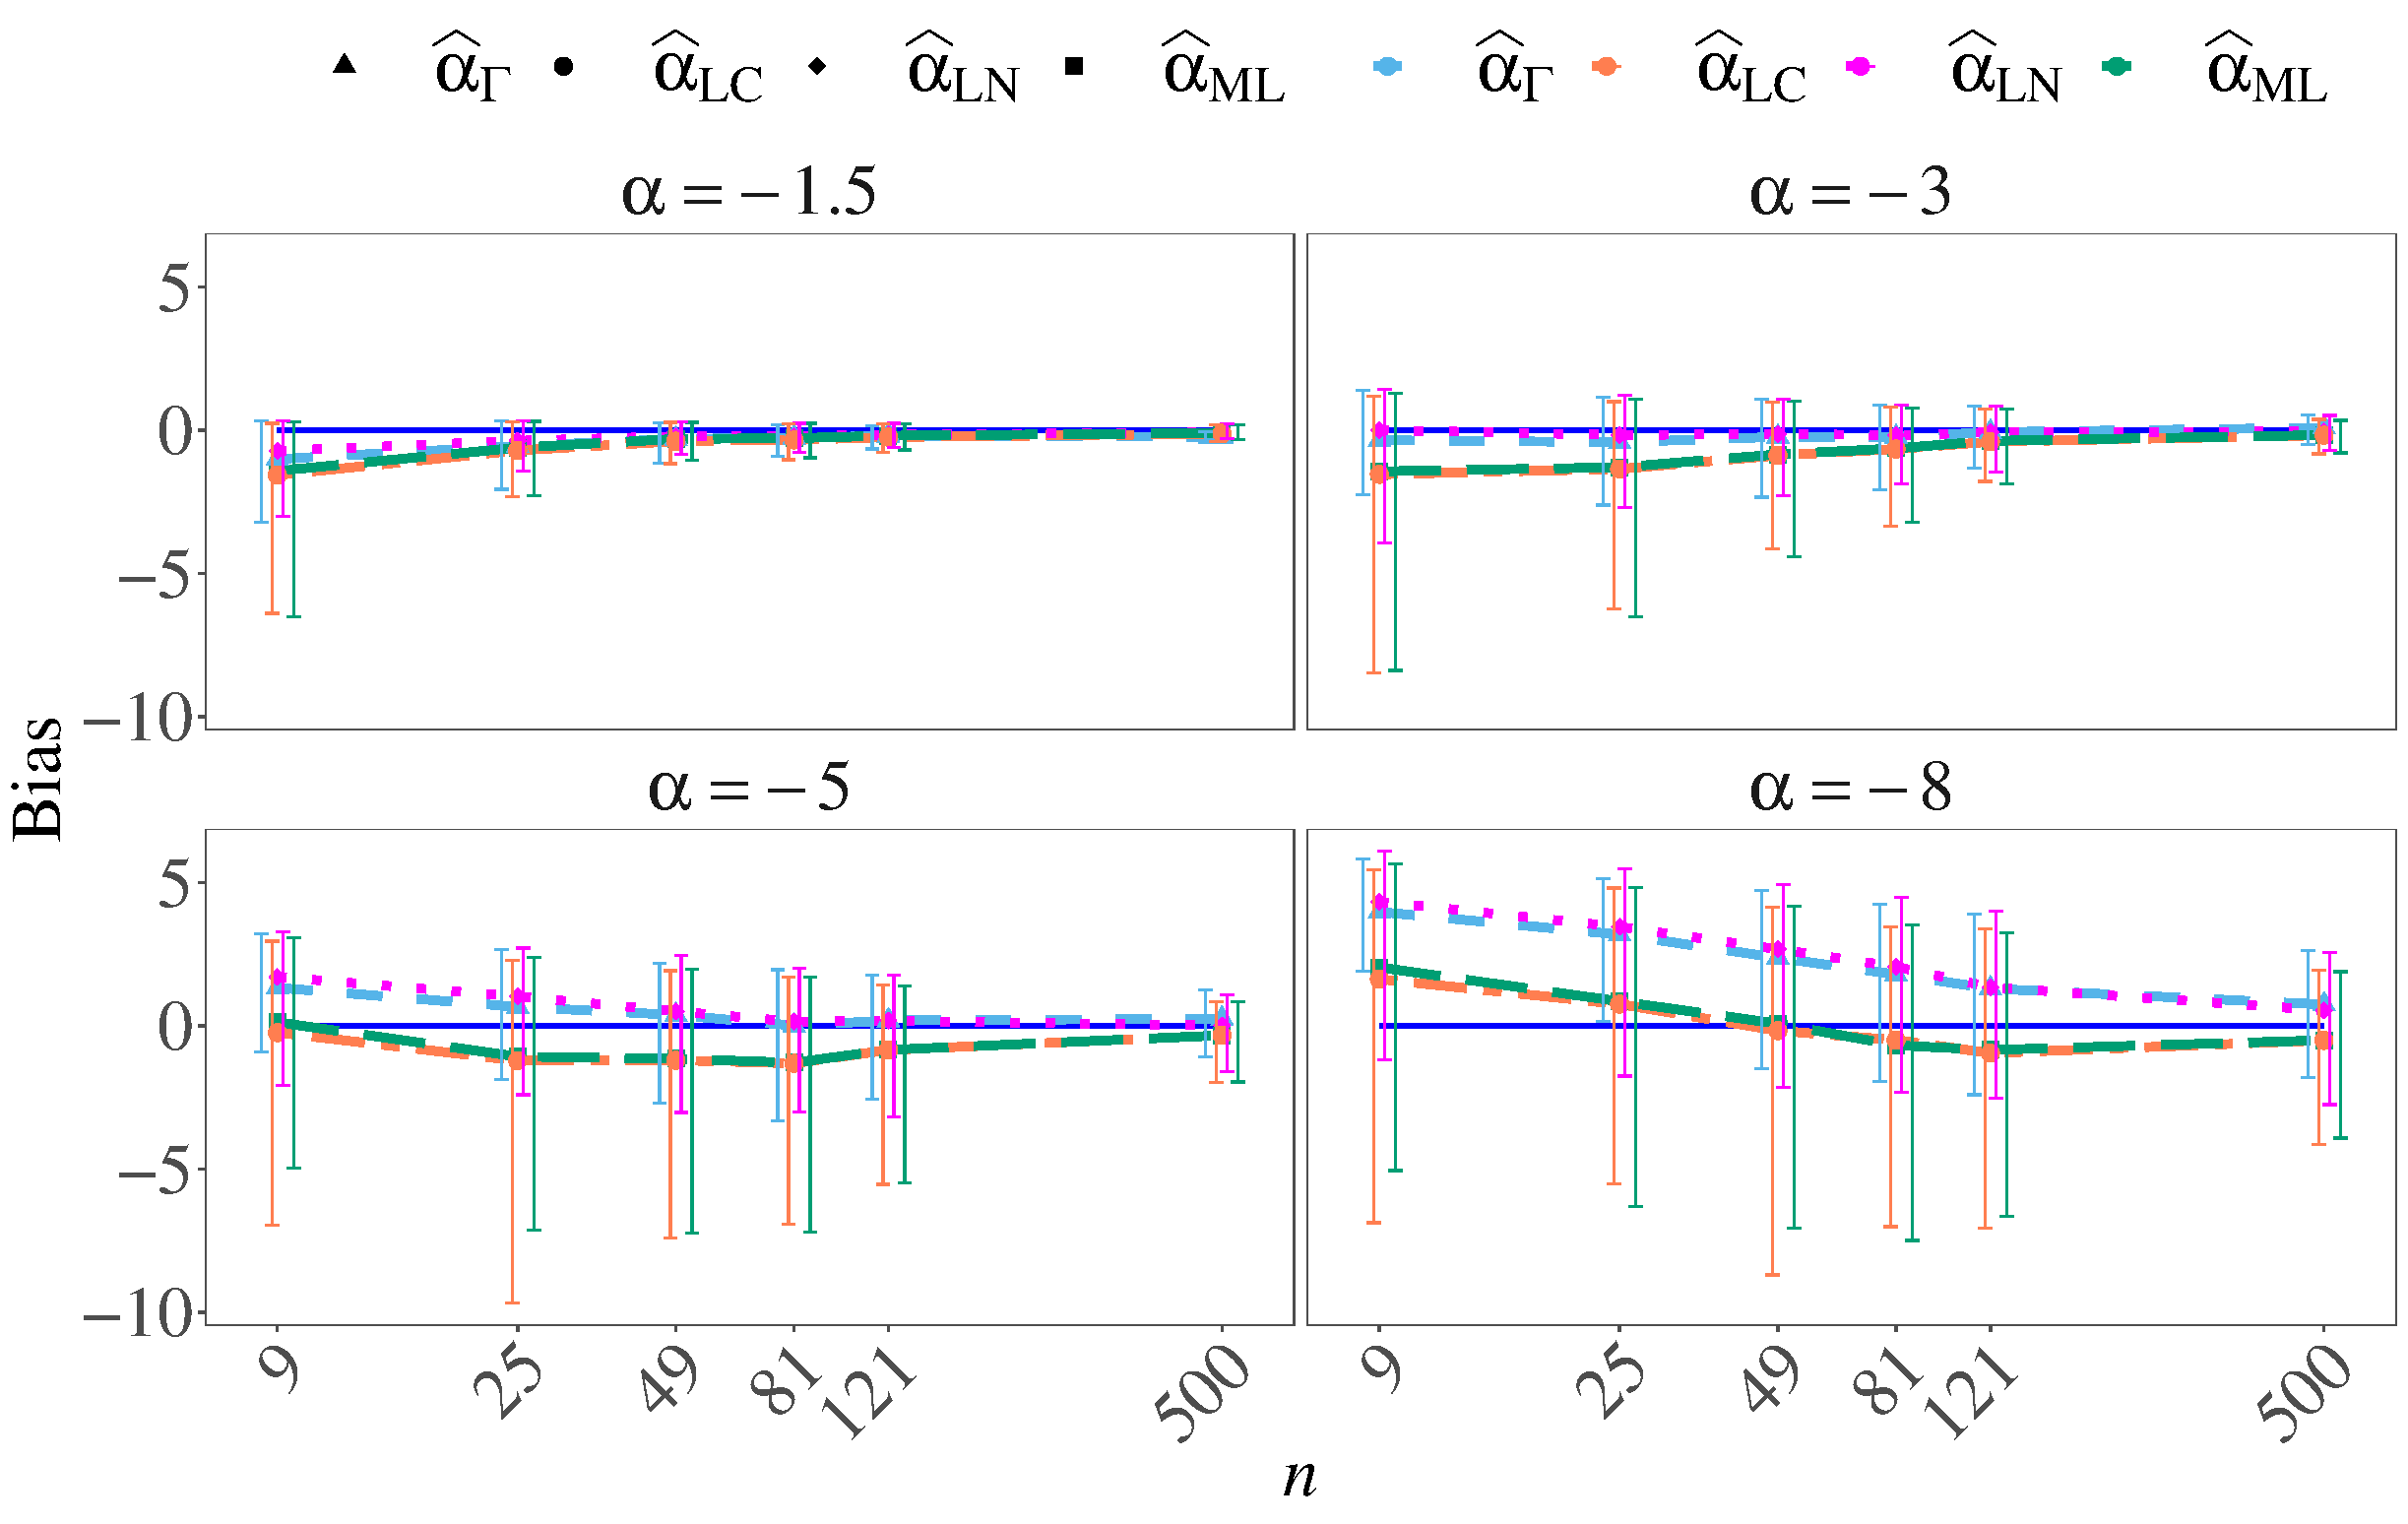
\includegraphics[width=.49\linewidth]{GraficoSesgoMVyGAyLNyLC_L=3Cont_BarrasErrorypercentil}}
\subfigure[\label{ECMConContL=3}$\widehat{\text{MSE}}$]{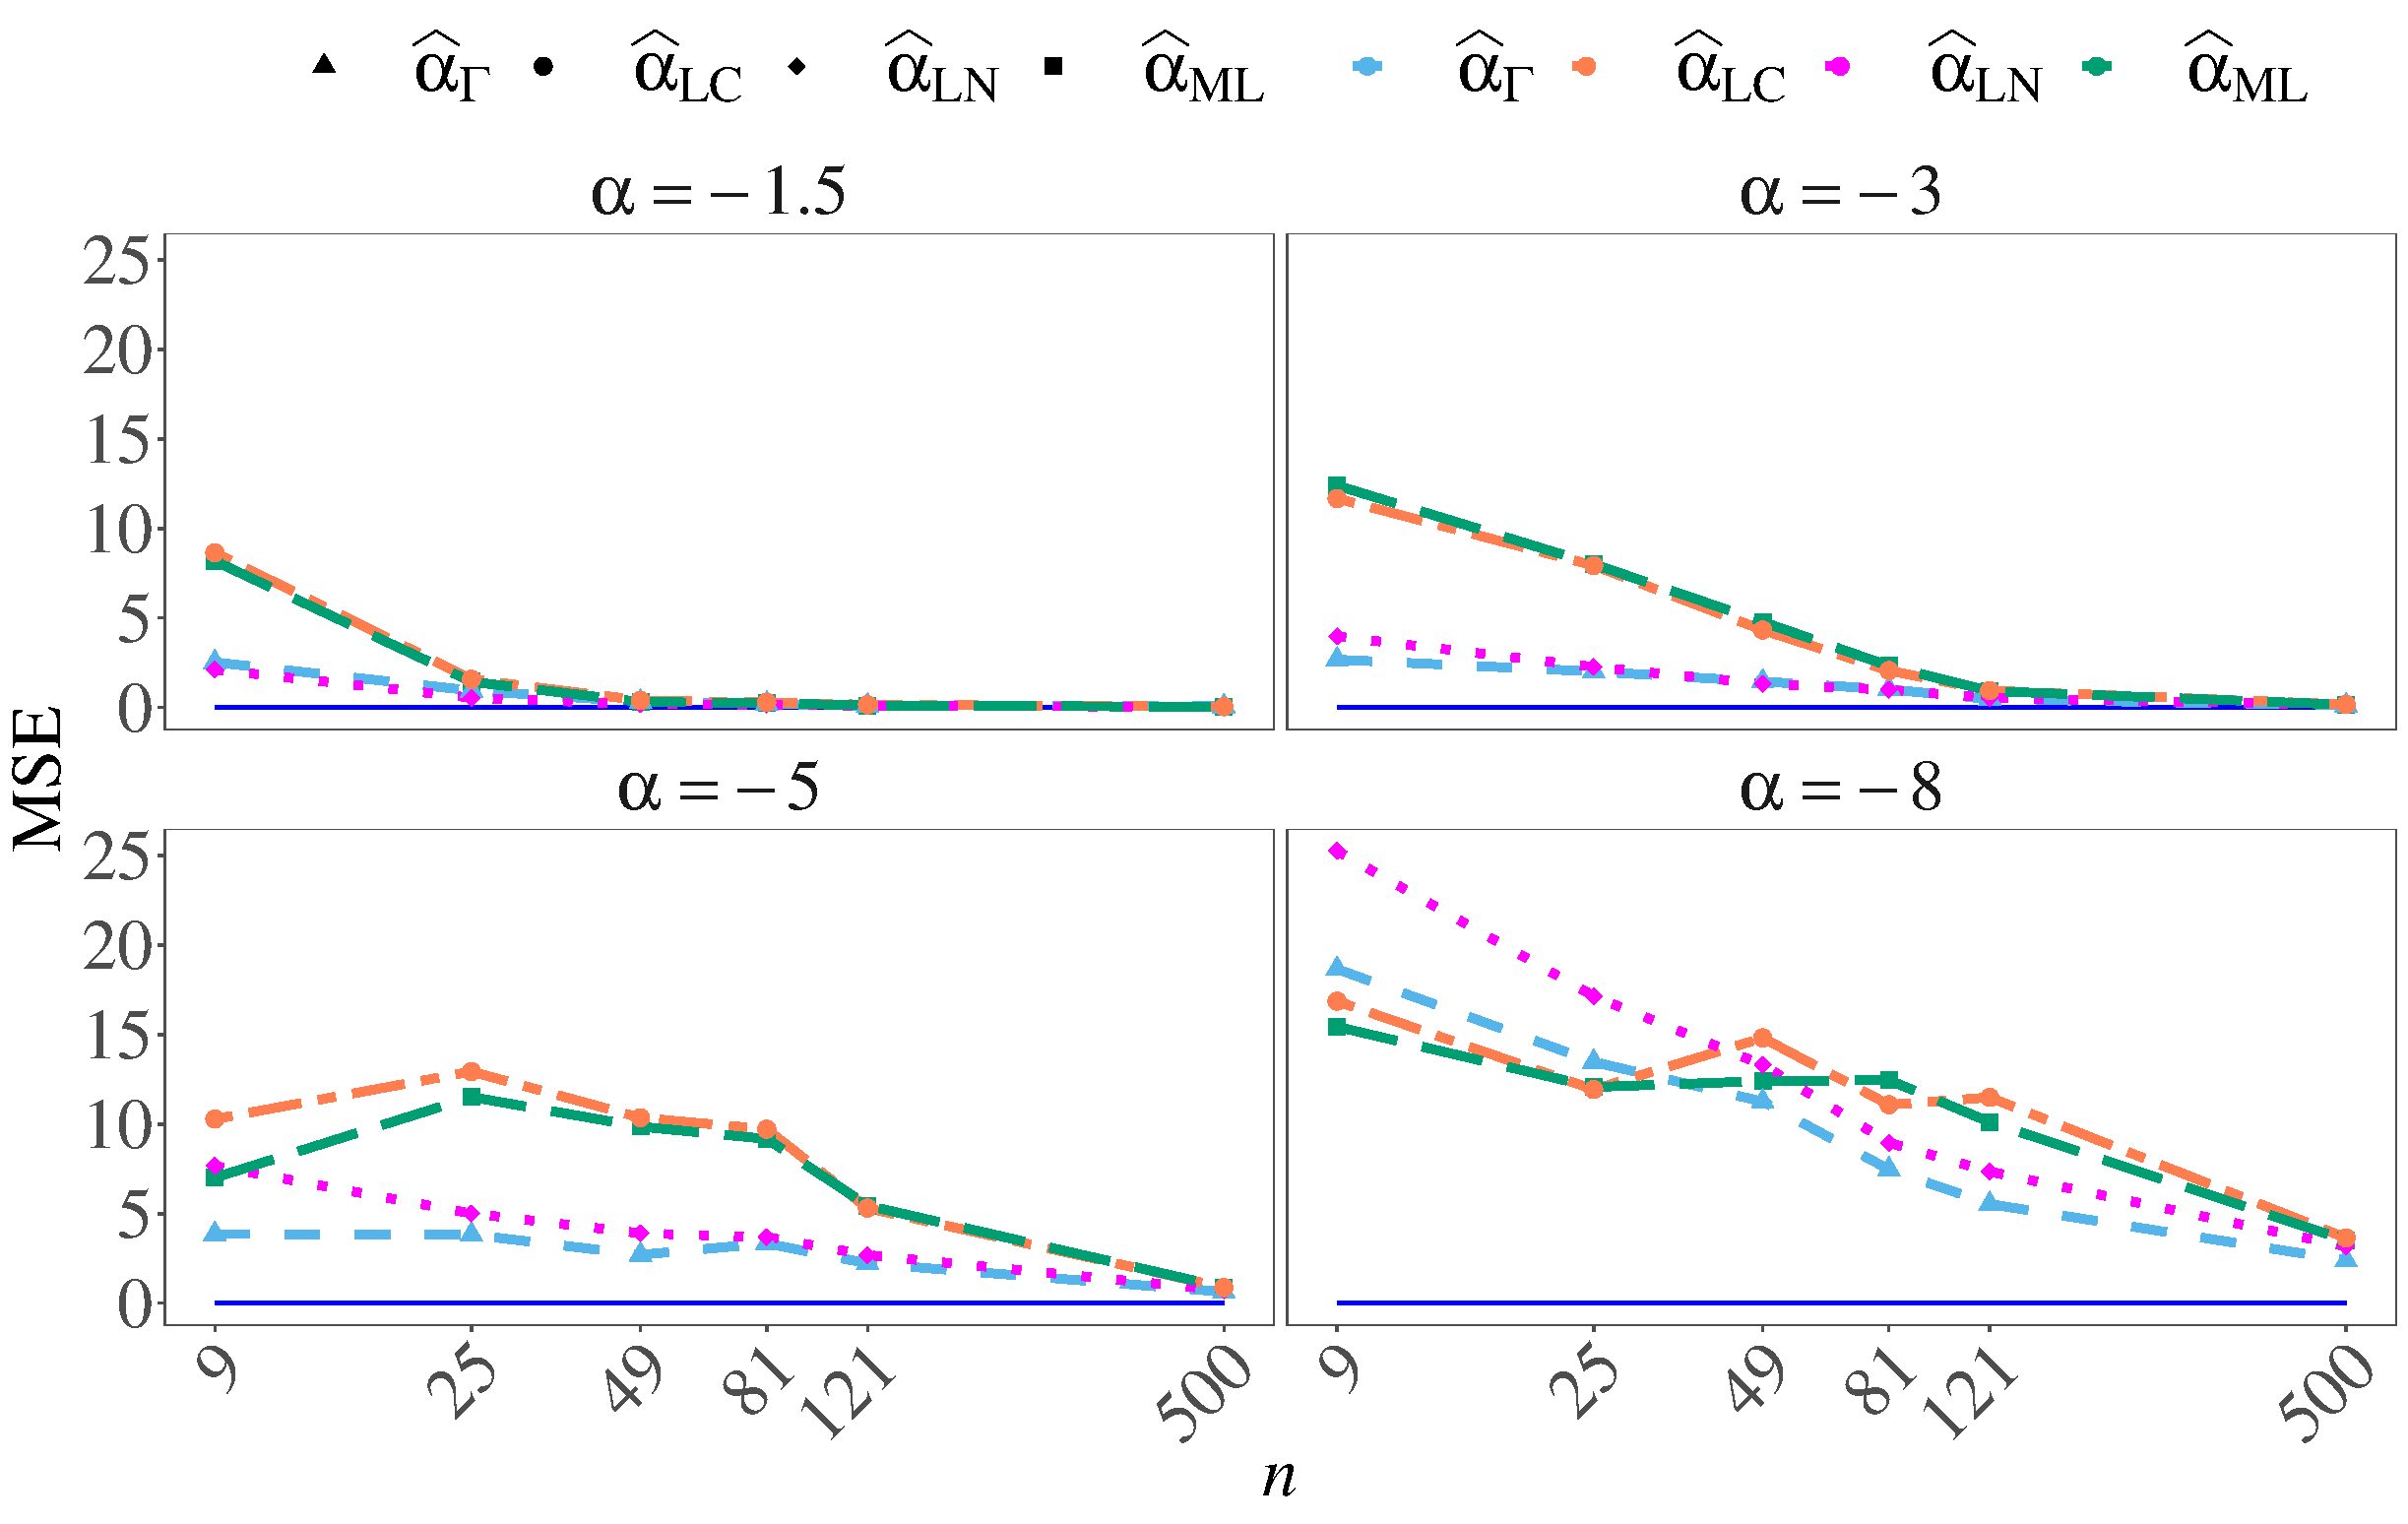
\includegraphics[width=.49\linewidth]{GraficoECMMVyGAyLNyLC_L=3Cont_BarrasErrorypercentil}}
\caption{Bias and MSE for contaminated data,  $\epsilon=0.05$ and $ L=3$.}\label{SesgoyECMConContL=3} 
\end{figure*}
%JC Programa: GraficoSesgoCont_L3BarrasError1ypercentil.R

\begin{figure*}[hbt]
\centering
\subfigure[\label{SesgoConContL=8}$\widehat{\text{Bias}}$]{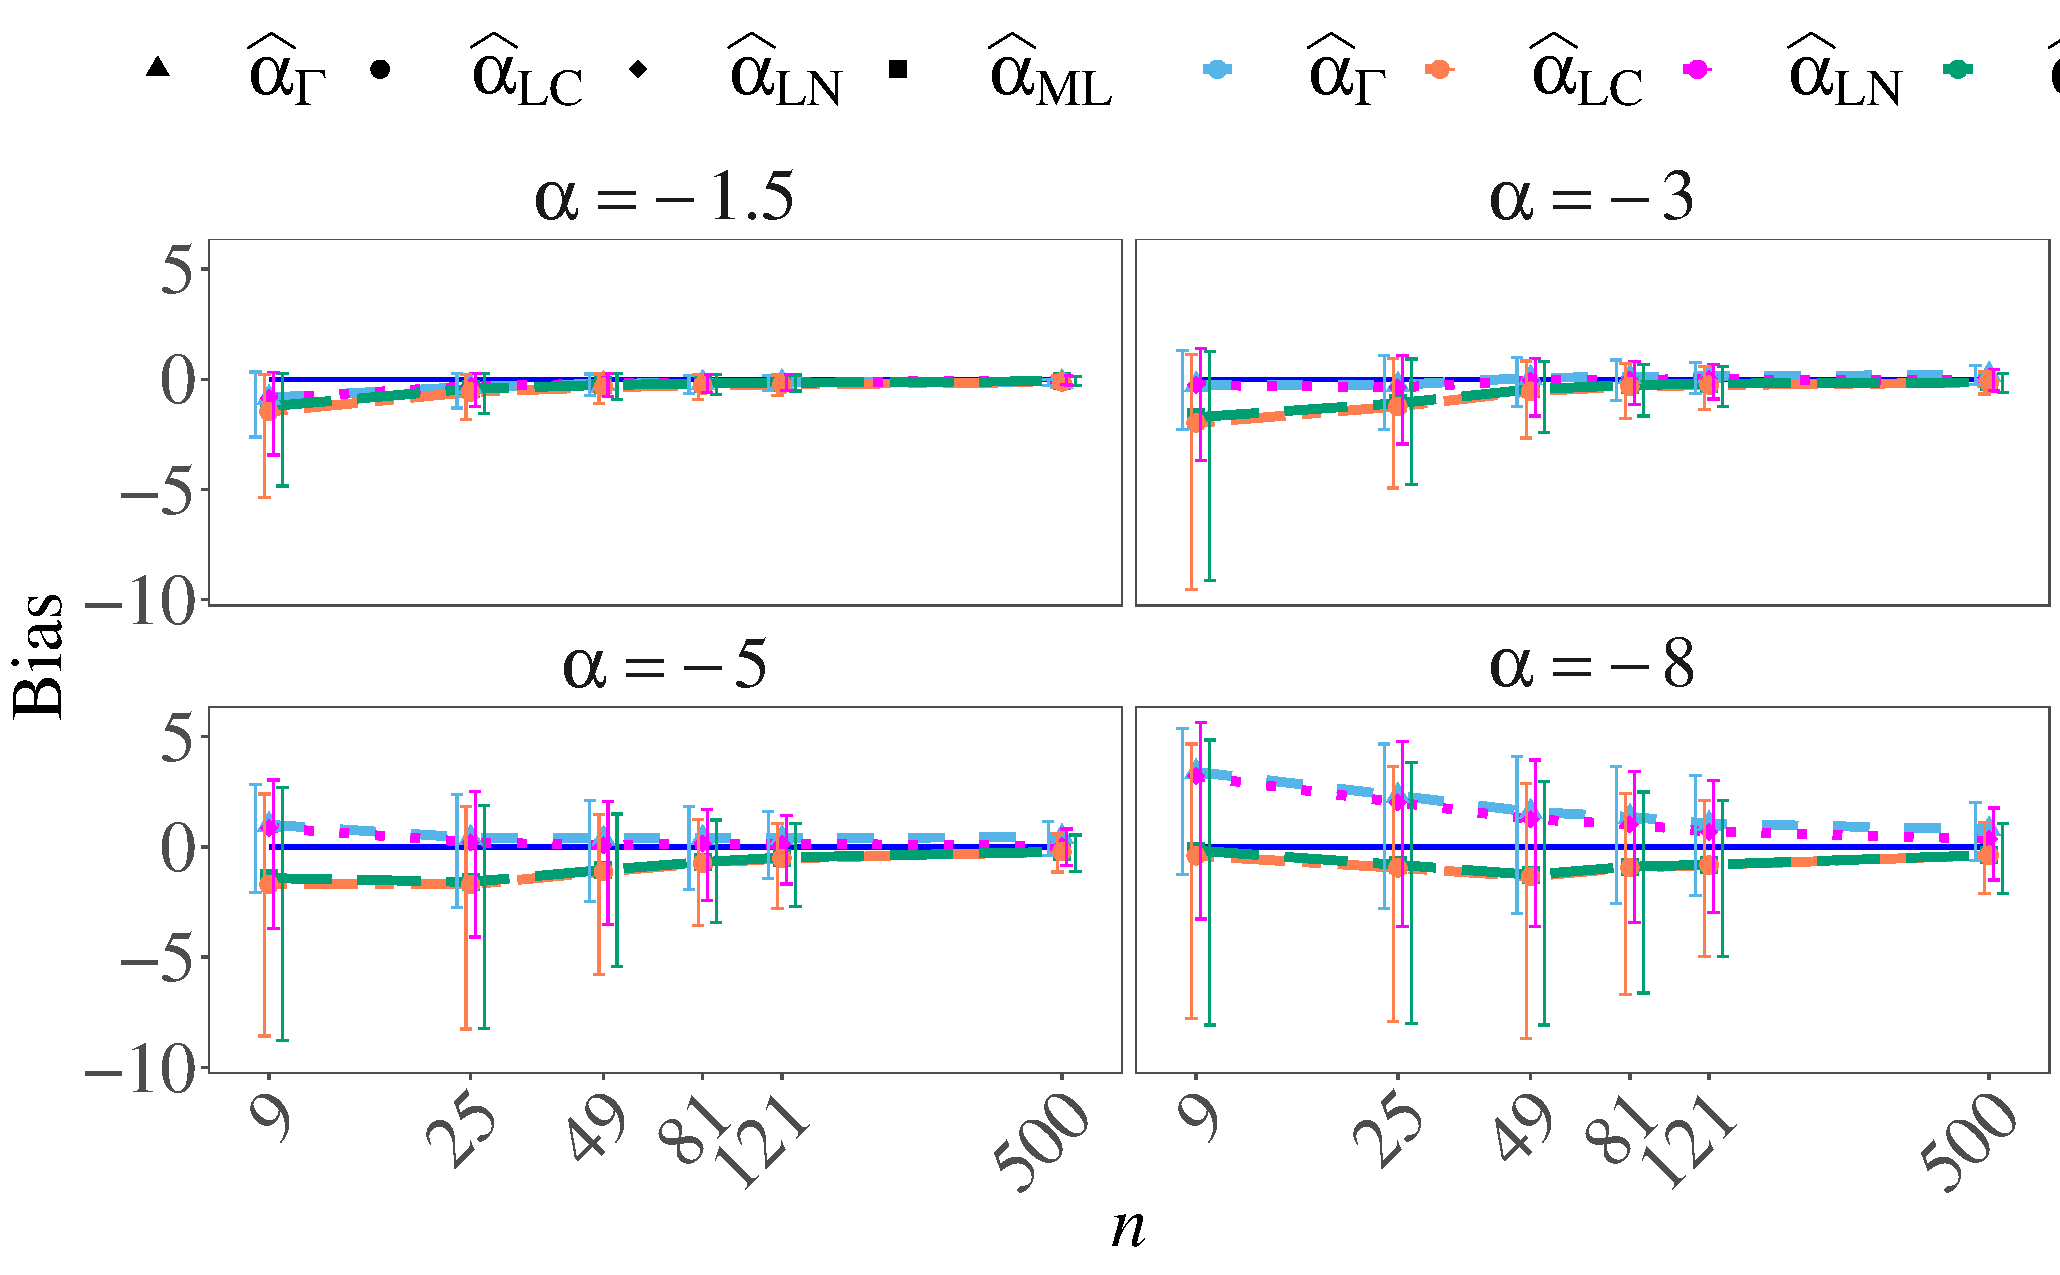
\includegraphics[width=.49\linewidth]{GraficoSesgoMVyGAyLNyLC_L=8Cont_BarrasErrorypercentil}}
\subfigure[\label{ECMConContL=8}$\widehat{\text{MSE}}$]{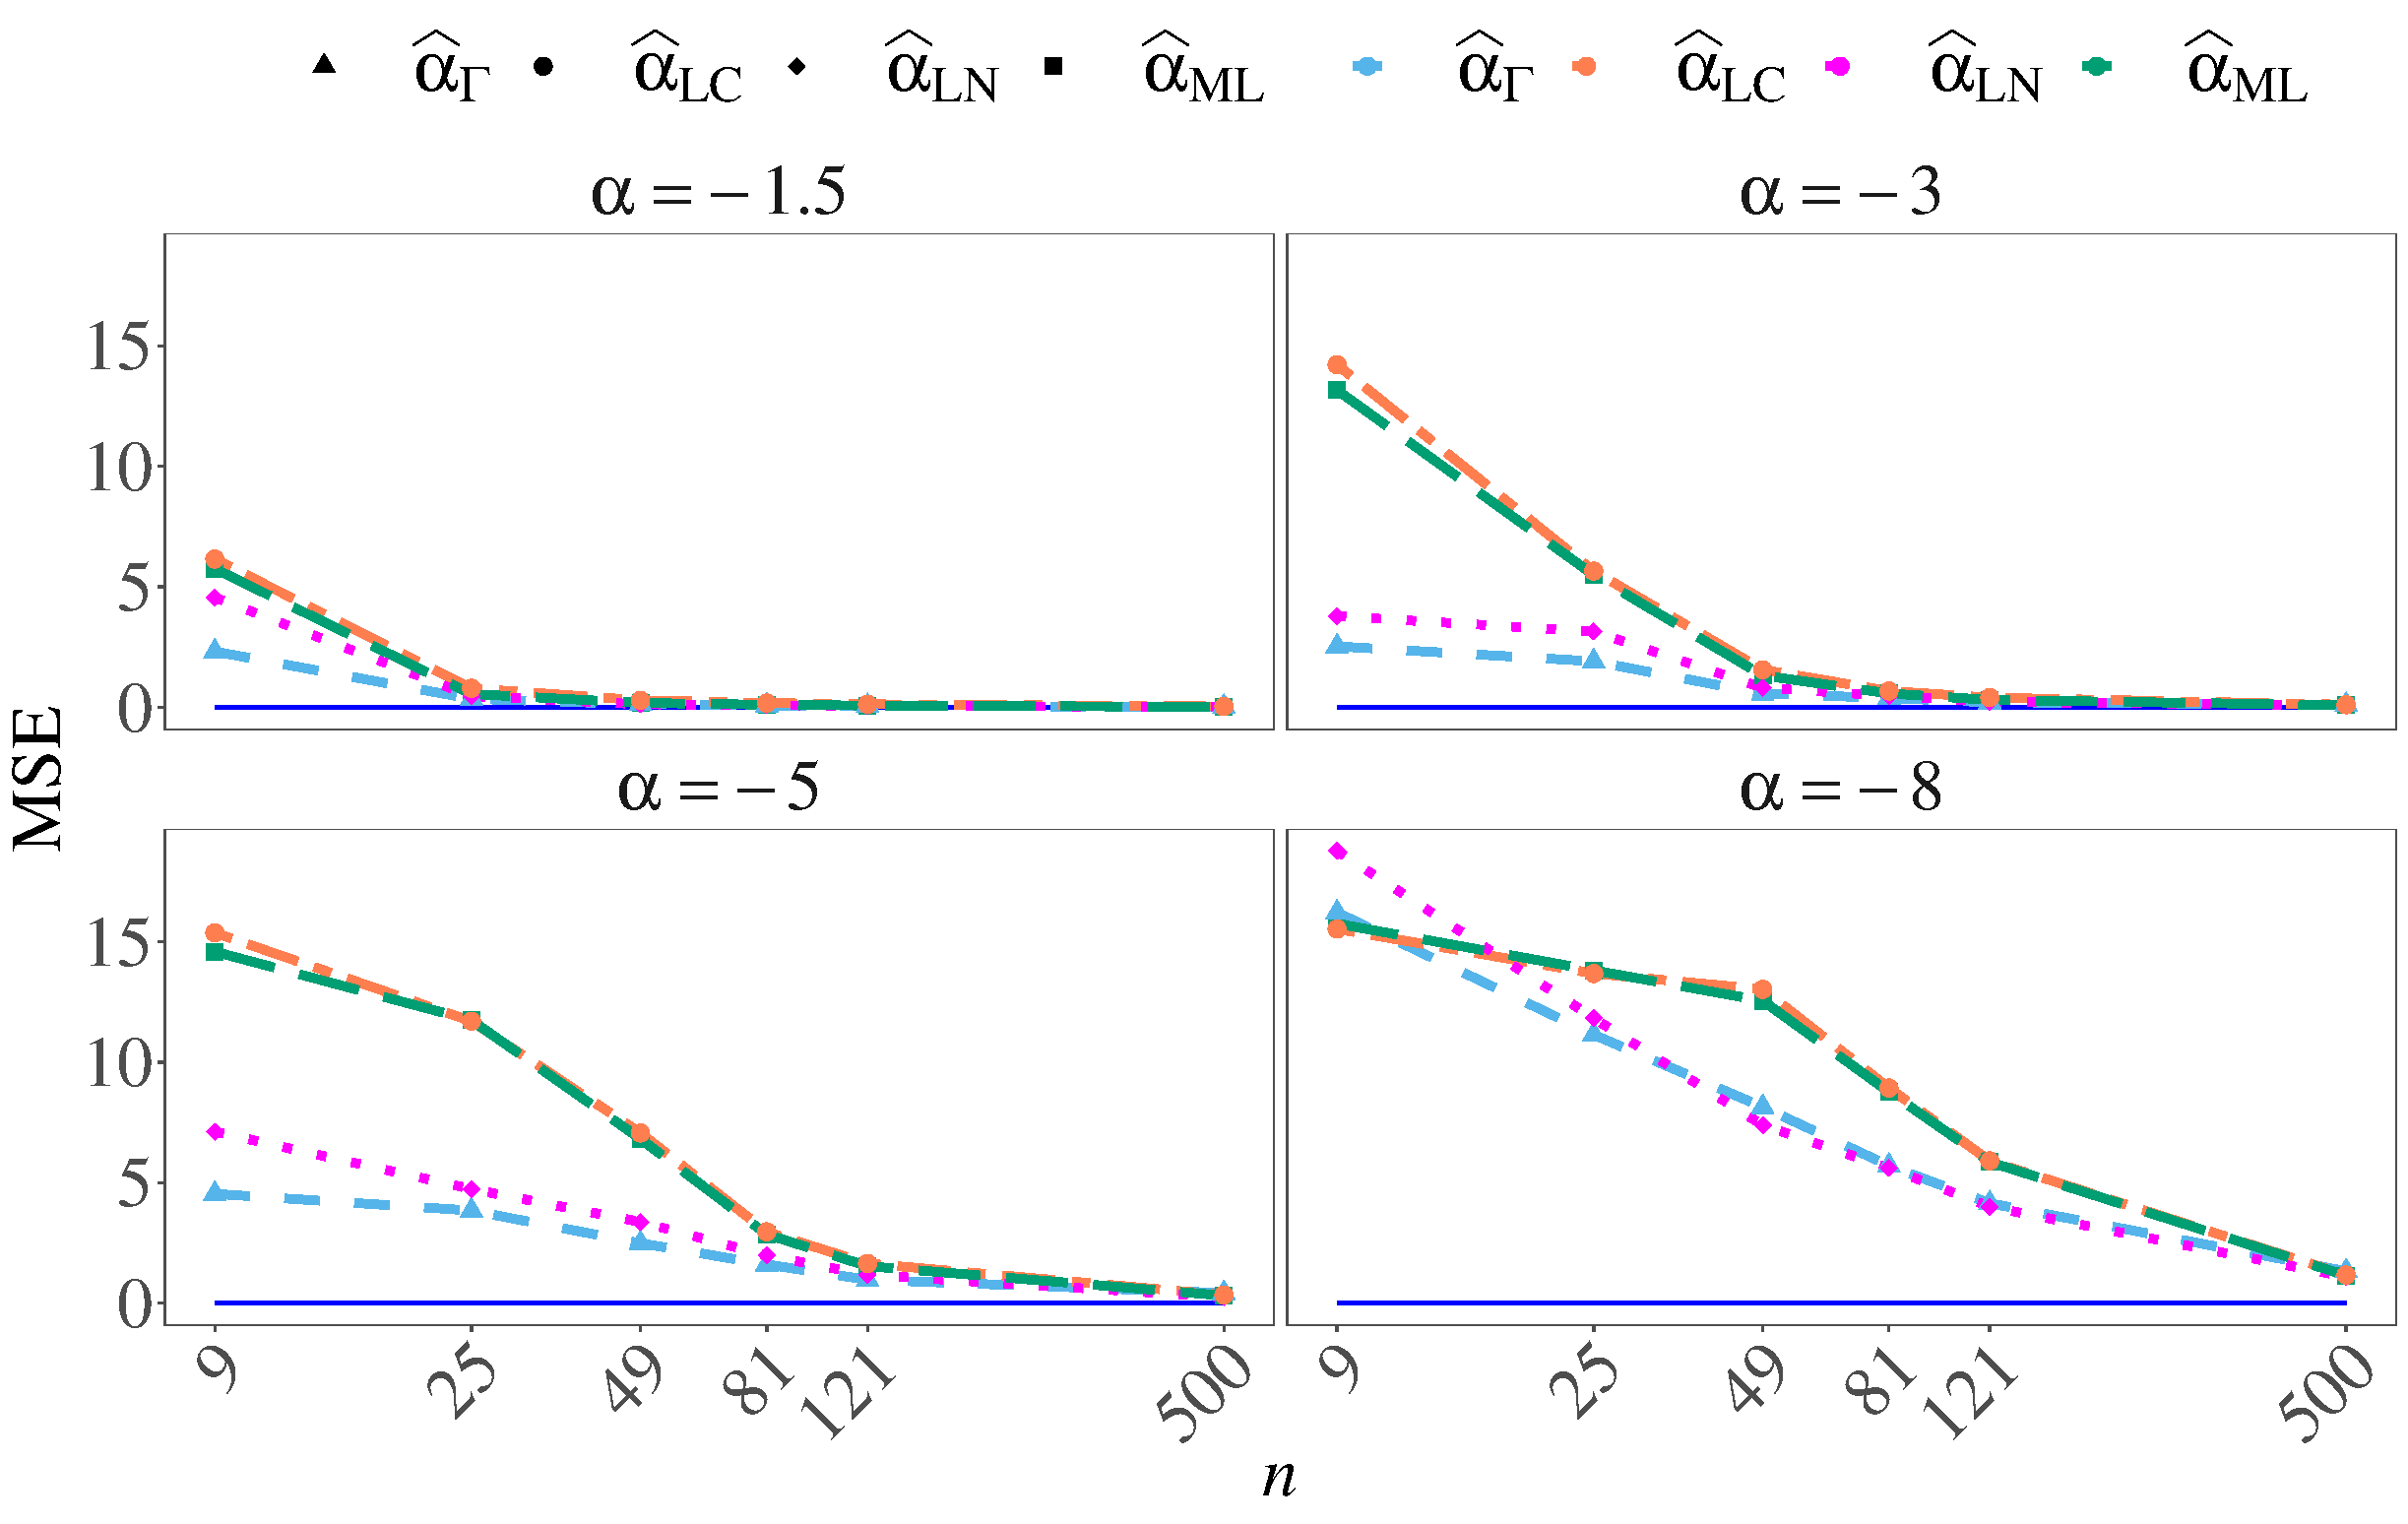
\includegraphics[width=.49\linewidth]{GraficoECMMVyGAyLNyLC_L=8Cont_BarrasErrorypercentil}}
\caption{Bias and MSE for contaminated data,  $\epsilon=0.05$ and $ L=8$.}\label{SesgoyECMConContL=8} 
\end{figure*}
%JC Programa: GraficoSesgoCont_L8BarrasError1ypercentil.R

At this level of contamination, it can be seen more clearly how the estimators are grouped by performance, $\widehat{\alpha}_{\text{{ML}}}$ and $\widehat{\alpha}_{\text{{LC}}}$ have suchlike behavior, while the same happens with $\widehat{\alpha}_{\Gamma}$ and $\widehat{\alpha}_{\text{{LN}}}$.  
The difference is noticeable, both in bias and in MSE, in favor of the MDE estimators for large values of $\alpha$. 
In the majority of the cases studied, the MDE estimators have shorter intervals than the other estimators. 
In moderately textured areas, all methods are comparable, although the MDE estimators have lower MSE than the classical ones. 
For homogeneous areas $\widehat{\alpha}_{\text{{ML}}}$ and $\widehat{\alpha}_{\text{{LC}}}$ have lower bias although greater variability.

\section{Application to actual data}
\label{application}

We applied the four estimation methods to an actual image from the surroundings of Munich, Germany, obtained by the E-SAR system~\cite{Horn1996} in L~band, HH~polarization, and intensity format. 
This image has $300\times250$ pixels and mainly comprises two different growth areas.

The original image is single-look.
To obtain comparable multilook data, we computed new pixels averaging the intensity values in $2\times2$ non-overlapping windows. This technique is known as pyramidal processing~\cite{Adelson1984}, and the resulting image is multilook.

The number of looks, defined by ${\text{E}(I)^2}/{\text{Var}(I)}$ in textureless areas, is not known, but it can be estimated by the equivalent number of looks (ENL) using uncorrelated data and the moment estimator
$\text{ENL}={1}/{\widehat{\text{CV}^2}}$, the reciprocal of the sample coefficient of variation $\widehat{\text{CV}}={\widehat{\sigma}}/{\widehat\mu}$, where $\widehat{\sigma}$ is the sample standard deviation and $\widehat\mu$ the sample mean.
In order to find the $\text{ENL}$ we selected manually four textureless areas and calculated $\text{ENL}_i$ for $i=1, \ldots, 4$. 
The final $\text{ENL}$ is their average weighted by the size of the areas. 
We then set $\widehat L=3.21$ in the analysis of the multilook image.

We found approximate confidence intervals at the \SI{95}{\percent} level with bootstrap and the percentile method~\cite{Davison1997}, using $2000$ independent replications.
This method uses the percentiles $\theta^*_{(\alpha)}$ and $\theta^*_{(1-\alpha)}$ of the distribution of $\widehat{\theta} $ generated by the bootstrap samples, where $\theta^*_{(\alpha)}$ and $\theta^*_{(1-\alpha)}$ are the sample percentiles of the distribution of $\widehat{\theta} $. 
According to Efron and Tibshirani~\cite{Efron93}, this method is preferable to the standard normal interval when there is evidence of non-normality.
Since our smallest sample size of interest is $n=9$, and the number of permutations is $n!=362880$, we obtained the bootstrap samples by uniform sampling $2000$ permutations.

\begin{figure}[hbt]
\centering
%\subfigure[\label{MuestraLooks}Samples used to estimate ENL]{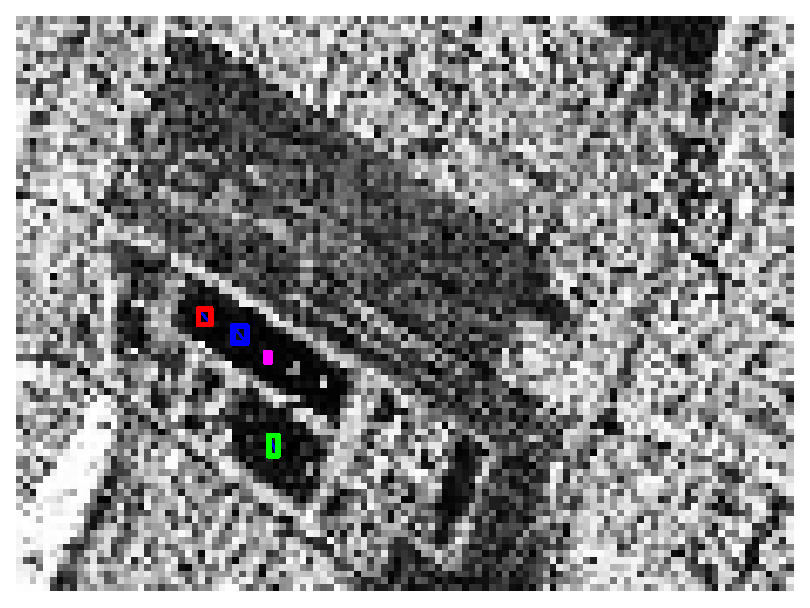
\includegraphics[width=0.48\linewidth]{MuestrasEstimNumLooks}}
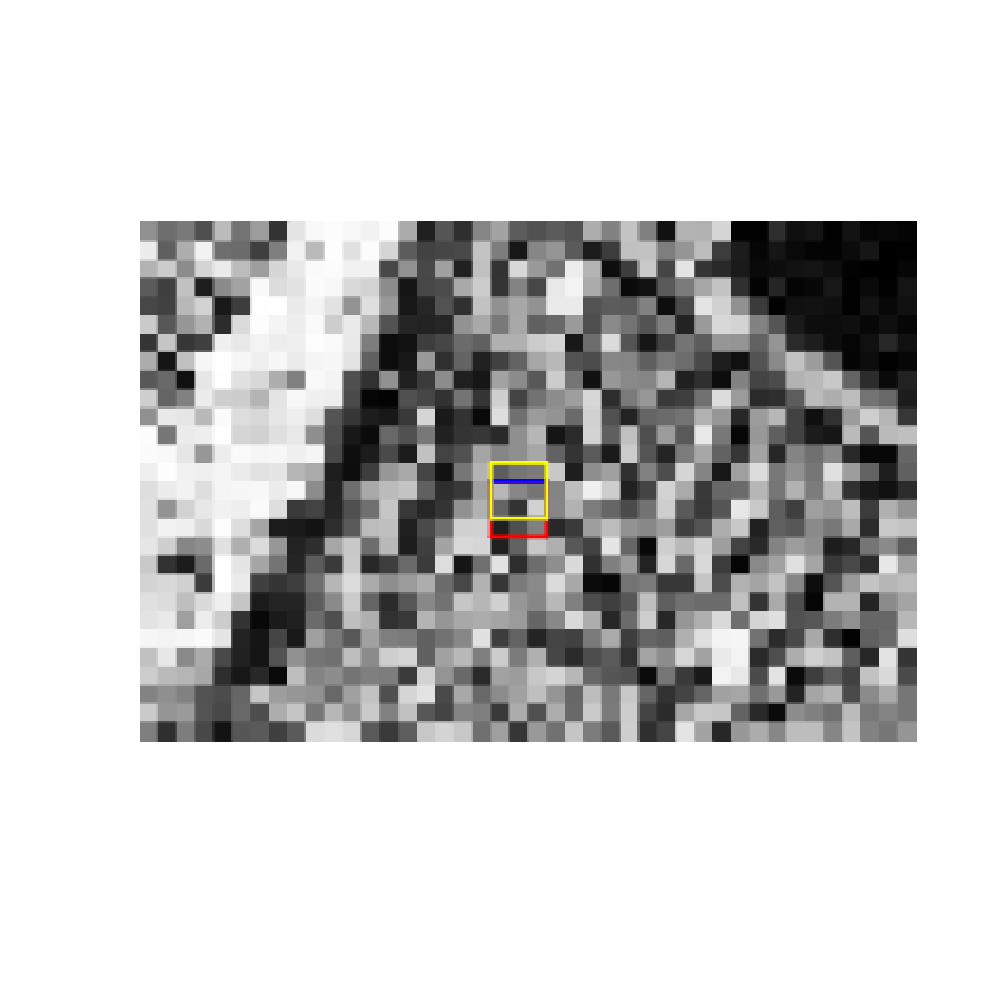
\includegraphics[width=0.8\linewidth]{TresMuestrasAgrandada}
\caption{Samples used to estimate $\widehat{\alpha}$.}\label{TresMuestras} 
\end{figure}
%JC Programa: GraficaTresMuestrasImagenESARUnPar_dlr_munichAgrandada.R

Figure~\ref{TresMuestras} shows three samples: yellow, red, and blue. 
The size of the first two is $16$, and the latter has a size $12$. 
The red sample is a shift from the yellow one in a row of the image data matrix, and the blue sample is contained within the yellow sample.

Table~\ref{TablaTresMuestras} shows the estimates obtained with the four methods in each sample. 
It can be seen that the estimates differ considerably in the yellow sample: 
both $\widehat{\alpha}_{\text{{ML}}}=-7.21$ and $\widehat{\alpha}_{\text{{LC}}}=-6.74$ are compatible with a homogeneous zone, while $\widehat{\alpha}_{\Gamma}=-4.34$ indicates that it is a heterogeneous one, and $\widehat{\alpha}_{\text{{LN}}}=-3.23$ is on the limit of affirming whether the area is heterogeneous or extremely heterogeneous.

On the one hand, both $\widehat{\alpha}_{\text{{ML}}}$ and $\widehat{\alpha}_{\text{{LC}}}$ have substantially changed the estimations value between the yellow and the red samples, indicating a different kind of textures. 
On the other hand, $\widehat{\alpha}_{\Gamma}$ and $\widehat{\alpha}_{\text{{LN}}}$ changed their values, but the type of zone they describe was not modified.

Table~\ref{TablaTresMuestras} also presents the bootstrap confidence intervals for each of the cases studied. 
It is important to mention that we only considered cases where the algorithm for the search of the texture parameter estimate converges. 
The final bootstrap sample size is indicated with the variable $n_b$ and it is mentioned as effective sample size.  
It can be observed that $\widehat{\alpha}_{\text{{LC}}}$ and $\widehat{\alpha}_{\text{{ML}}}$ methods yielded the smallest effective sample sizes, and that the most accurate confidence intervals were achieved by $\widehat{\alpha}_{\text{{LN}}}$.
These results suggest that this last method is the most dependable in term of algorithm convergence. 

\begin{table*}[hbt]
\centering
\caption{Estimates of $\widehat{\alpha}_{\text{{ML}}}$, $\widehat{\alpha}_{\Gamma}$, $\widehat{\alpha}_{\text{{LN}}}$ and $\widehat{\alpha}_{\text{{LC}}}$ for three samples from the ESAR image, along with their bootstrap confidence intervals and effective bootstrap sample sizes ($n_b$).}\label{TablaTresMuestras}
\begin{tabular}{c*5{c}}
	\toprule
	Color       &  $n$    &  $\widehat{\alpha}_{\text{{ML}}}$    &  $\widehat{\alpha}_{\Gamma}$  &  $\widehat{\alpha}_{\text{{LN}}}$ &  $\widehat{\alpha}_{\text{{LC}}}$\\
	\cmidrule(lr){1-6}
	Yellow      & $16$  & $-7.21$ & $-4.34$ & $-3.23$ & $-6.74$\\
	&	& $[-17.4;-2.47]$ & $[-11.5;-1.88]$ & $[-9.40;-1.64]$ & $[-14.5;-1.86]$\\
	$n_{b}$    	& & 1392          & 1894          & 1926          &  1250        \\ \midrule
	Red         & $16$  & $-3.04$ & $-3.42$ & $-2.12$ & $-3.27$\\
	& & $[-12.4;-1.72]$ & $[-10.3;-1.74]$ & $[-4.88;-1.43]$ & $[-12.0;-1.60]$\\
	$n_{b}$    	& & 1924          & 1948          & 1988          & 1586         \\ \midrule
	Blue        & $12$  & $-4.62$ & $-3.85$ & $-2.35$ & $-4.52$\\
	& & $[-15.5;-1.88]$ & $[-11.9;-1.68]$ & $[-7.46;-1.44]$ & $[-14.4;-1.59]$\\
	$n_{b}$    & & 1615          & 1879          & 1968          & 1376         \\
	\bottomrule
\end{tabular}
\end{table*} 


%\begin{table}[hbt]
%	\addtolength{\tabcolsep}{-4pt}
%	\centering
%	\caption{Confidence intervals and effective bootstrap sample sizes for the estimates of $\widehat{\alpha}_{\text{{ML}}}$, $\widehat{\alpha}_{\Gamma}$, $\widehat{\alpha}_{\text{{LN}}}$ and $\widehat{\alpha}_{\text{{LC}}}$ from Table~\ref{TablaTresMuestras}.}\label{ICTresMuestras}
%	\begin{tabular}{c*4{c}}
%		\toprule
%		Color       &  $\widehat{\alpha}_{\text{{ML}}}$    &  $\widehat{\alpha}_{\Gamma}$  &  $\widehat{\alpha}_{\text{{LN}}}$ &  $\widehat{\alpha}_{\text{{LC}}}$\\
%		\cmidrule(lr){1-5}
%		Yellow      & $[-17.4;-2.47]$ & $[-11.5;-1.88]$ & $[-9.40;-1.64]$ & $[-14.5;-1.86]$\\
%		$n_{b}$    & 1392          & 1894          & 1926          &  1250        \\
%		\cmidrule(lr){1-5}
%		Red         & $[-12.4;-1.72]$ & $[-10.3;-1.74]$ & $[-4.88;-1.43]$ & $[-12.0;-1.60]$\\
%		$n_{b}$    & 1924          & 1948          & 1988          & 1586         \\
%		\cmidrule(lr){1-5}
%		Blue        & $[-15.5;-1.88]$ & $[-11.9;-1.68]$ & $[-7.46;-1.44]$ & $[-14.4;-1.59]$\\
%		$n_{b}$    & 1615          & 1879          & 1968          & 1376         \\
%		\bottomrule
%	\end{tabular}
%\end{table} 

Then, based on the results of the simulations obtained for the SEIF corresponding to Figures~\ref{InflL3alfa-3n25} and~\ref{InflL3alfa-3n25}, that show the lack of robustness of $\widehat{\alpha}_{\text{{ML}}}$ and $\widehat{\alpha}_{\text{{LC}}}$ when contaminated with a small value, we re-estimate this parameter removing the smallest observation that corresponds to a value \SI{86}{\percent} lower than the average. 
Table~\ref{SinPrimero} shows the estimates after this censoring.

\begin{table*}[hbt]
\centering
\caption{Estimates of $\widehat{\alpha}_{\text{{ML}}}$, $\widehat{\alpha}_{\Gamma}$, $\widehat{\alpha}_{\text{{LN}}}$ y $\widehat{\alpha}_{\text{{LC}}}$ in the yellow sample without the smallest observation, along with their bootstrap confidence intervals and effective bootstrap sample sizes ($n_b$).}\label{SinPrimero} 
\begin{tabular}{c*4{c}}
	\toprule
	&  $\widehat{\alpha}_{\text{{ML}}}$    &  $\widehat{\alpha}_{\Gamma}$  &  $\widehat{\alpha}_{\text{{LN}}}$ &  $\widehat{\alpha}_{\text{{LC}}}$\\
	\cmidrule(lr){2-5}
	& $-5.73$   & $-3.97$    & $-3.13$    & $-4.81$\\
	& $[-16.9;-2.21]$ & $[-12.0;-1.80]$ & $[-10.2;-1.644]$ & $[-15.0;-1.70]$\\
	$n_{b}$	& 1538          & 1913           & 1940          &  1371 \\
	\bottomrule
\end{tabular}
\end{table*}

Again, it can be observed a significant change in the estimated values of the $\widehat{\alpha}_{\text{{ML}}}$ and $\widehat{\alpha}_{\text{{LC}}}$, giving now estimates compatible with a homogeneous zone. This shows the robustness of the stochastic distance estimator against the $\widehat{\alpha}_{\text{{ML}}}$ and $\widehat{\alpha}_{\text{{LC}}}$ estimators.
The table also presents the bootstrap confidence intervals and the effective sample sizes $n_b$. 
We observe the same behaviour as before: $\widehat{\alpha}_{\text{{LN}}}$ has the largest $n_b$ and the shortest confidence interval.

%\begin{table}[hbt]
%	\addtolength{\tabcolsep}{-4pt}
%	\centering
%	\caption{ $\widehat{\alpha}_{\text{{ML}}}$, $\widehat{\alpha}_{\Gamma}$, $\widehat{\alpha}_{\text{{LN}}}$ and $\widehat{\alpha}_{\text{{LC}}}$ confidence interval of table~\ref{SinPrimero} estimations.}\label{ICYellowSinOutlier}
%	\textcolor{blue}{
%		\begin{tabular}{c*4{c}}
	%			\toprule
	%			& $\widehat{\alpha}_{\text{{ML}}}$    &  $\widehat{\alpha}_{\Gamma}$  &  $\widehat{\alpha}_{\text{{LN}}}$ &  $\widehat{\alpha}_{\text{{LC}}}$\\
	%			\cmidrule(lr){1-5}
	%			&[-16.9;-2.21] & [-12.0;-1.80] & [-10.2;-1.644] & [-15.0;-1.70]\\
	%			$n_{b}$       & 1538          & 1913           & 1940          &  1371 \\
	%			\bottomrule
	%		\end{tabular}
%	}
%\end{table} 

We performed another analysis of the behavior of the estimation methods with the five samples shown in Figure~\ref{CincoMuestras}. 
We chose nested squared samples of sides $n=9,25,49,81$ and $121$. 
Figure~\ref{AlfaVsTamCincoMuestras} shows the estimates $\widehat{\alpha}$ for each method and each sample as functions of the sample size $n$. 

\begin{figure}[hbt]
\centering
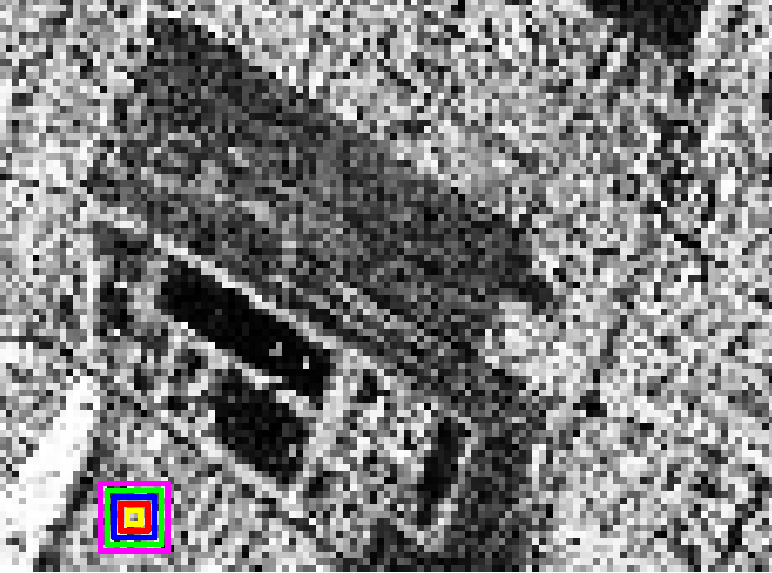
\includegraphics[width=0.7\linewidth]{CincoMuestras}
\caption{Five samples used to compare $\widehat{\alpha}_{\text{{ML}}}$, $\widehat{\alpha}_{\Gamma}$, $\widehat{\alpha}_{\text{{LN}}}$ and  $\widehat{\alpha}_{\text{{LC}}}$.}\label{CincoMuestras}
\end{figure}
%JC Programa: GraficaTresMuestrasImagenESARUnPar_dlr_munichAgrandada.R

\begin{figure}[hbt]
\centering
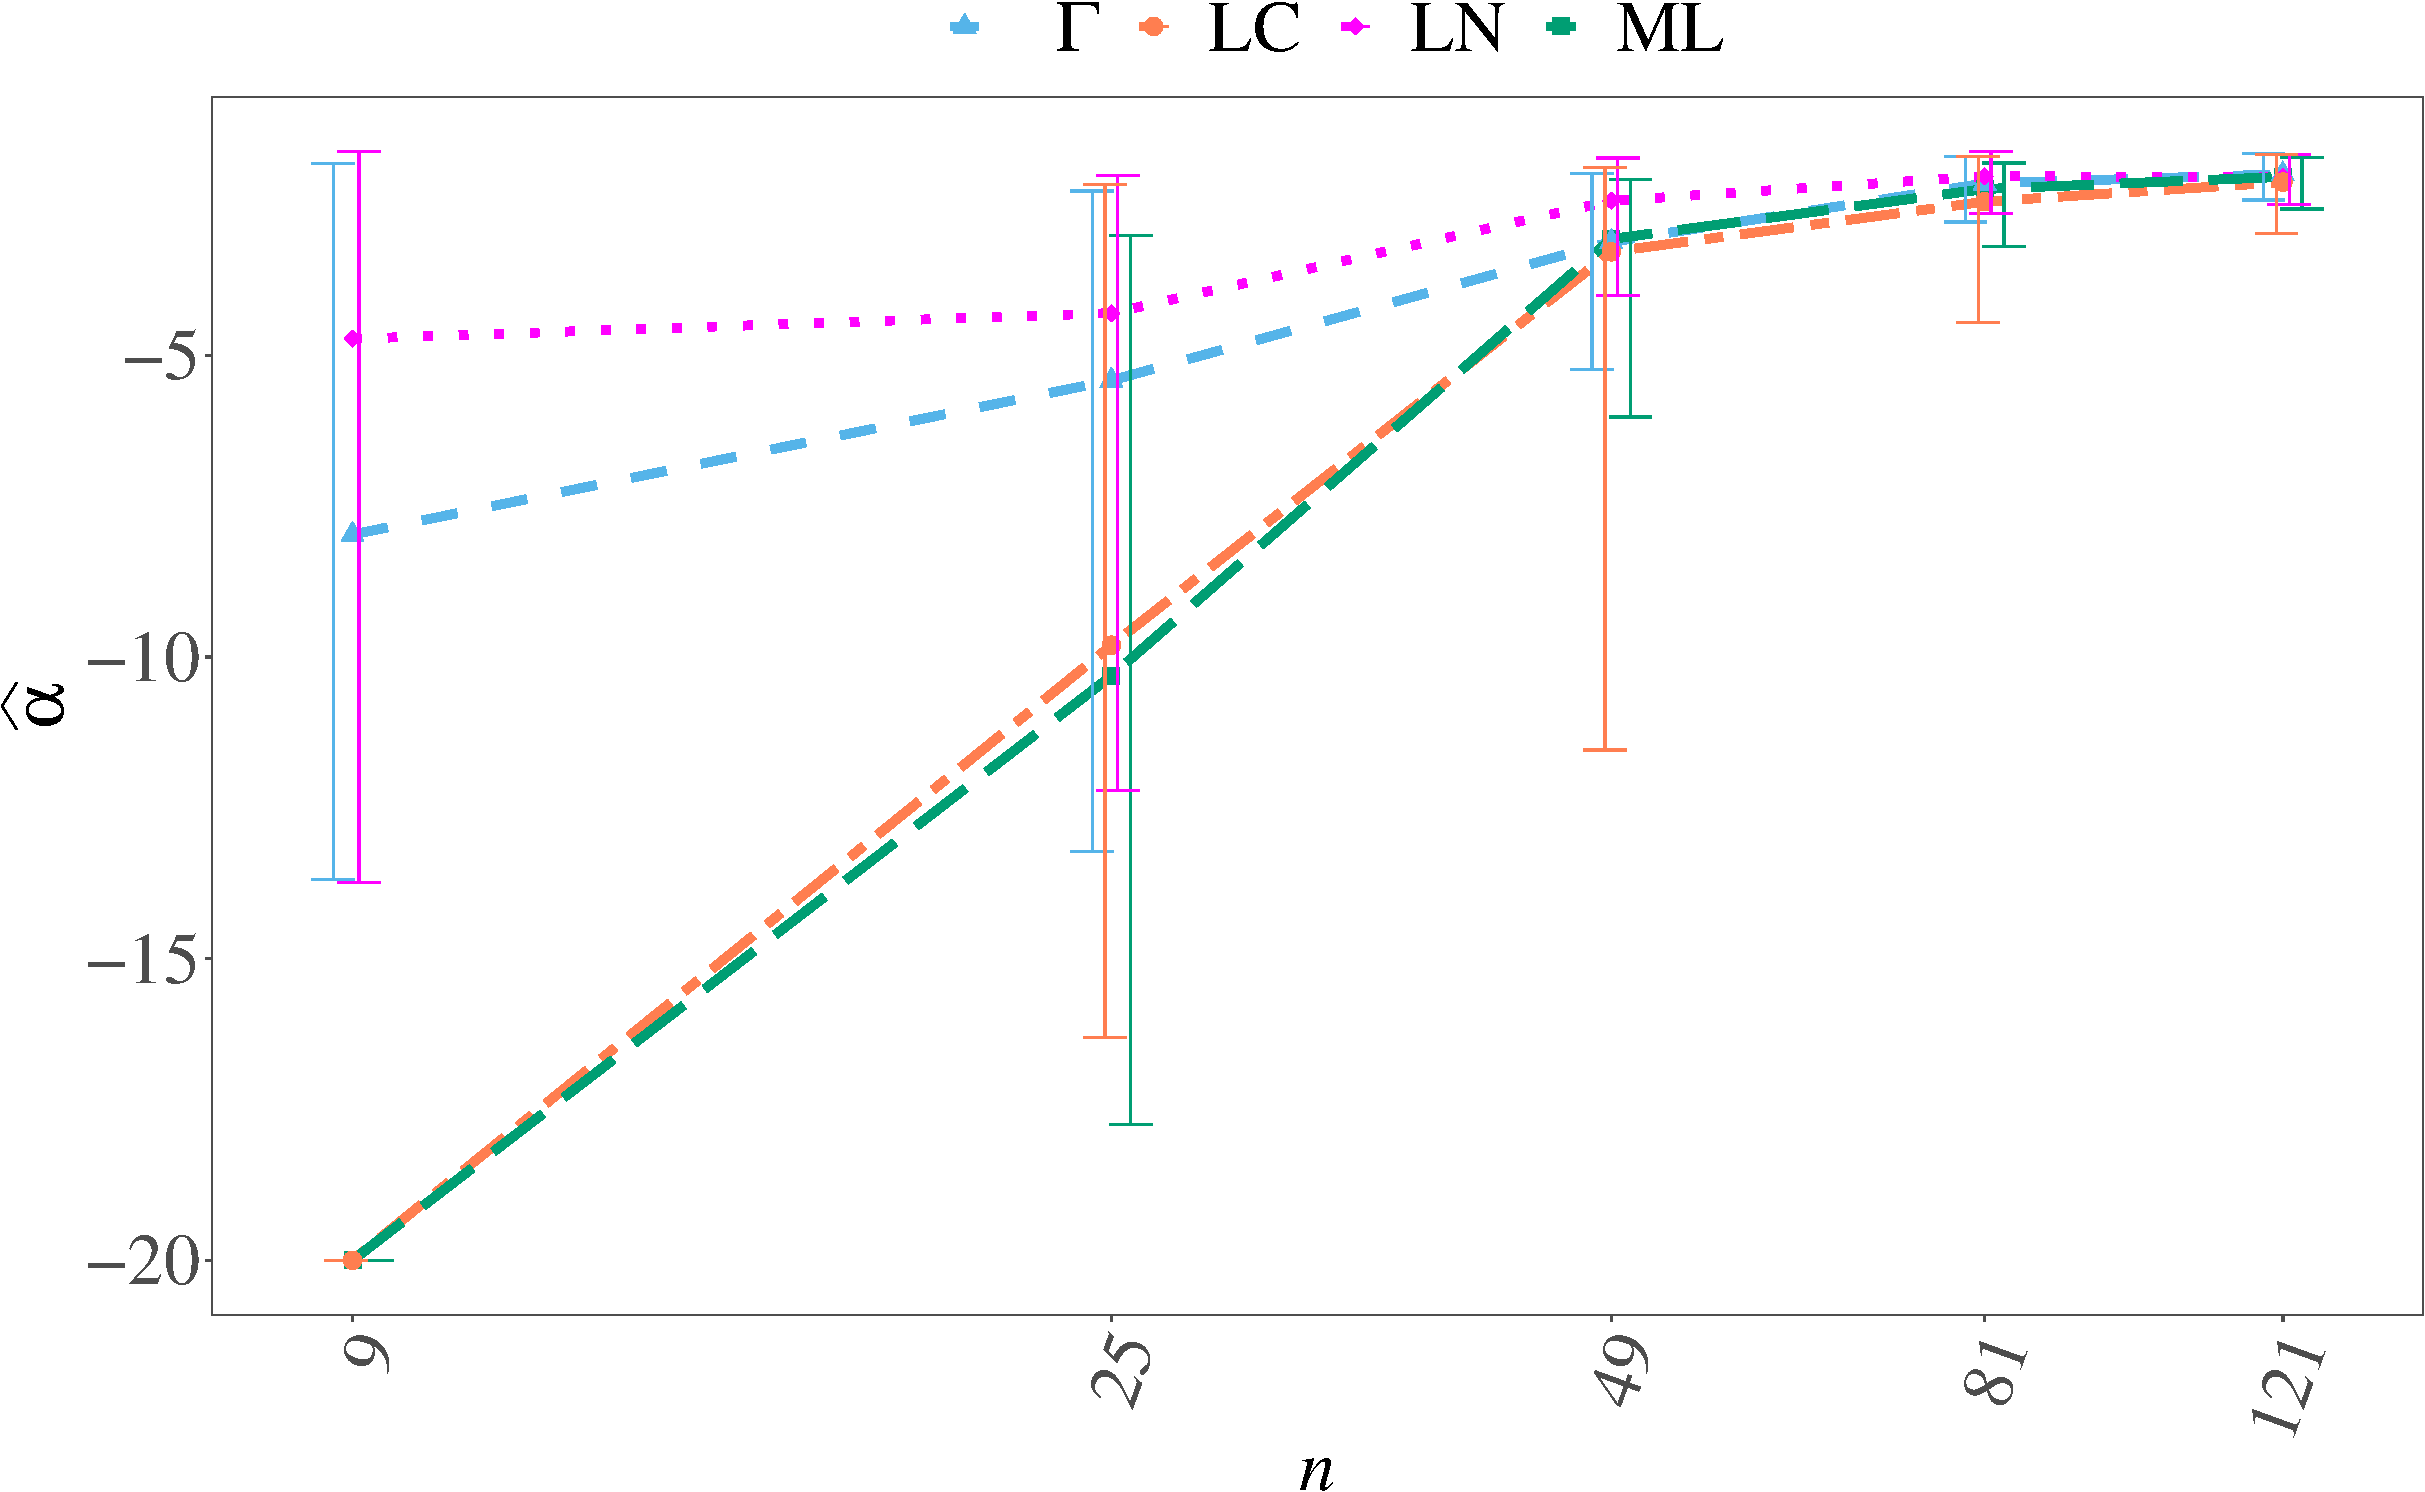
\includegraphics[width=\linewidth]{AlfaVsTamCincoMuestrasCorregido_v2}
\caption{ $\widehat{\alpha}_{\text{{ML}}}$, $\widehat{\alpha}_{\Gamma}$, $\widehat{\alpha}_{\text{{LN}}}$ and $\widehat{\alpha}_{\text{{LC}}}$ for corresponding samples to image~\ref{CincoMuestras}.}\label{AlfaVsTamCincoMuestras}
\end{figure}
%JC programa: GraficoAlfaEstvs_n_ImagenReal_Corregido.R

Table~\ref{TablaCincoMuestras} shows the estimates, along with the confidence intervals and effective bootstrap sample sizes (denoted as $n_b$).
It can be seen that $\widehat{\alpha}_{\text{{ML}}}$ and $\widehat{\alpha}_{\text{{LC}}}$ have similar performance, and so have $\widehat{\alpha}_{\text{{LN}}}$ and $\widehat{\alpha}_{\Gamma}$. 
For $n= 9$ none of the ML and LC methods converge, thus the value $-20$. 
As the sample size increases, the estimates stabilize, showing that the LN method is the most stable while $\widehat{\alpha}_{\text{{ML}}}$ and $\widehat{\alpha}_{\text{{LC}}}$ are the most unstable, giving poor estimates for small sample sizes.
It can also be observed that $n_b$ is smaller for MC and LC methods for small sample sizes, suggesting that these techniques are more prone to numerical instabilities in such cases.


%\begin{table}[hbt]
%	\centering
%	\caption{Estimates of ${\alpha}$ for the five nested samples shown in Fig.~\ref{CincoMuestras}.}\label{TablaCincoMuestras} 
%	\begin{tabular}{c*5{r}}
%		\toprule
%		Color       &  $n$    &  $\widehat{\alpha}_{\text{{ML}}}$    &  $\widehat{\alpha}_{\Gamma}$  &  $\widehat{\alpha}_{\text{{LN}}}$ &  $\widehat{\alpha}_{\text{{LC}}}$\\
%		\cmidrule(lr){1-6}
%		Yellow      & $9$     & $-20.00$      & $-7.97$ & $-4.73$ & $-20.00$\\
%		Red         & $25$    & $-10.31$  & $-5.42$ & $-4.30$ & $-9.81$\\
%		Blue        & $49$    & $-3.07$   & $-3.12$ & $-2.44$ & $-3.28$\\
%		Green       & $81$    & $-2.24$   & $-2.15$ & $-2.03$ & $-2.45$\\
%		Magenta     & $121$   & $-2.04$   & $-1.99$ & $-2.05$ & $-2.13$\\
%		\bottomrule
%	\end{tabular}
%\end{table}

\begin{table*}[hbt]
\centering
\caption{Estimates of $\widehat{\alpha}_{\text{{ML}}}$, $\widehat{\alpha}_{\Gamma}$, $\widehat{\alpha}_{\text{{LN}}}$ and $\widehat{\alpha}_{\text{{LC}}}$ for five nested samples from the ESAR image, along with their bootstrap confidence intervals and effective bootstrap sample sizes ($n_b$).}\label{TablaCincoMuestras}
\begin{tabular}{c*5{c}}
	\toprule
	Color       &  $n$    &  $\widehat{\alpha}_{\text{{ML}}}$    &  $\widehat{\alpha}_{\Gamma}$  &  $\widehat{\alpha}_{\text{{LN}}}$ &  $\widehat{\alpha}_{\text{{LC}}}$\\
	\cmidrule(lr){1-6}
	Yellow      & $9$     & $-20.00$      & $-7.97$           & $-4.73$          & $-20.00$\\
	&	      & -             & $[-13.69;-1.83]$  & $[-13.74;-1.63]$ & -\\
	$n_{b}$    	&         &   $857$       & $1642$            &  $1740$          & $947$         \\ \midrule
	Red         & $25$  & $-10.31$        & $-5.42$           & $-4.30$          & $-9.81$\\
	&                   & $[-17.75;-3.02]$ & $[-13.22;-2.28]$  & $[-12.22;-2.02]$ & $[-16.30;-2.16]$\\
	$n_{b}$    	&       &  $1332$         & $1900$            &  $1957$          &   $1159$       \\ \midrule
	Blue        & $49$  & $-3.07$         & $-3.12$         & $-2.44$         &  $-3.28$\\
	&       & $[-6.02;-2.08]$ & $[-5.24;-1.98]$ & $[-4.01;-1.73]$ & $[-11.54;-1.89]$\\
	$n_{b}$    	&       & $1997$          &  $1999$         &   $2000$        &  $1893$        \\ \midrule
	Green       & $81$  & $-2.24$         & $-2.15$         & $-2.03$         & $-2.45$\\
	&       & $[-3.20;-1.82]$ & $[-2.79;-1.70]$ & $[-2.65;-1.63]$ & $[-4.46;-1.70]$\\
	$n_{b}$    	&       & $2000$          &  $2000$         &  $2000$         & $1997$         \\ \midrule
	Magenta     & $121$ & $-2.04$         & $-1.99$        & $-2.05$          & $-2.13$\\
	&       & $[-2.58;-1.73]$ & $[-2.43;-1.66]$ & $[-2.50;-1.67]$ & $[-2.99;-1.67]$\\
	$n_{b}$    	&       &  $2000$         &  $2000$         &  $2000$         &  $2000$        \\ \midrule
	\bottomrule
\end{tabular}
\end{table*} 
In Table~\ref{tab:LongIC} we see the length of the confidence intervals depicted in Fig.~\ref{AlfaVsTamCincoMuestras}.
In most cases, the ML and LC produce wider intervals than those from other methods. 
All the widths decrease as the sample size increases; that is, estimates become progressively more precise. 
It is noteworthy that the shortest confidence interval corresponds to the LN method in most cases. 
It should be noted that there is no confidence interval for the cases where ML and LC methods did not converge.
It is important to clarify that this analysis is performed for small samples corresponding to the chosen windows sizes. 

\begin{table}[htb]
\centering
\caption{\label{tab:LongIC}Length of bootstrap confidence intervals showed in Fig.\ref{AlfaVsTamCincoMuestras}}
\begin{tabular}{*5{r}}
	\toprule 
	$n$     &  $\widehat{\alpha}_{\text{{ML}}}$    &  $\widehat{\alpha}_{\Gamma}$  &  $\widehat{\alpha}_{\text{{LN}}}$ &  $\widehat{\alpha}_{\text{{LC}}}$ \\
	\midrule
	9     &    ---  & 11.86 & 12.12 & --- \\
	25    & 14.74 & 10.94 & 10.20 & 14.14 \\
	49    & 3.94  & 3.25  & 2.28  & 9.65 \\
	81    & 1.38  & 1.09  & 1.03  & 2.75 \\
	121   & 0.85  & 0.77  & 0.83  & 1.31 \\
	\bottomrule
\end{tabular}
\end{table}%



%	\begin{table}[hbt]
%		\centering
%		\caption{Estimates of ${\alpha}$ for the five nested samples shown in Fig.~\ref{CincoMuestras}.}\label{TablaCincoMuestras} 
%		\begin{tabular}{c*5{r}}
	%			\toprule
	%			Color       &  $n$    &  $\widehat{\alpha}_{\text{{ML}}}$    &  $\widehat{\alpha}_{\Gamma}$  &  $\widehat{\alpha}_{\text{{LN}}}$ &  $\widehat{\alpha}_{\text{{LC}}}$\\
	%			\cmidrule(lr){1-6}
	%			Yellow      & $9$     & $-20.00$      & $-7.97$ & $-4.73$ & $-20.00$\\
	%			Red         & $25$    & $-10.31$  & $-5.42$ & $-4.30$ & $-9.81$\\
	%			Blue        & $49$    & $-3.07$   & $-3.12$ & $-2.44$ & $-3.28$\\
	%			Green       & $81$    & $-2.24$   & $-2.15$ & $-2.03$ & $-2.45$\\
	%			Magenta     & $121$   & $-2.04$   & $-1.99$ & $-2.05$ & $-2.13$\\
	%			\bottomrule
	%		\end{tabular}
%	\end{table}

Figure~\ref{CornerReflector} shows the same ESAR image with a corner reflector in a dark background. 
We selected nested samples to estimate $\alpha$; only the two largest (in yellow and red) include the corner reflector.
Table~\ref{ResultadosCorner} shows the estimates, the confidence interval and the effective bootstrap sample size $n_b$.
None of the estimators converge for $n=9$. 
For the rest of the sample sizes, LN estimator is the most stable. 
Furthermore, the LN estimator does not show any change between the green sample and the yellow sample, which contain the corner reflector. 
All the other methods showed changes in the estimation by changing the type of texture from one sample to another. 
That is the kind of stability sought for a good estimator for these kinds of problems of image processing and understanding. 
It is important to note that the confidence intervals are larger than those presented in Table~\ref{TablaCincoMuestras}, a likely effect of the corner reflector.

\begin{figure}[hbt]
\centering
\includegraphics[width=\linewidth]{CornerJulia_Roja}
\caption{Nested samples with and without a corner reflector.}\label{CornerReflector}
\end{figure}
%JC Programa: ImagenESARUnPar_dlr_munich_RecoradaCorner.R


%\begin{table}[hbt]
%	\caption{Estimated $\widehat{\alpha}$ in nested boxes.}\label{ResultadosCorner} 
%	%\begin{tabular}{c 5*(c c c c c)}
%	\begin{tabular}{c r S[table-number-alignment = right] S[table-number-alignment = right] S[table-number-alignment = right] S[table-number-alignment = right]}
%		\toprule
%		Color & $n$ &  ${\widehat\alpha}_{\text{MV}}$ & ${\widehat{\alpha}_{\Gamma}}$ &${\widehat\alpha}_{\text{{LN}}}$  &${\widehat\alpha}_{\text{{LC}}}$ \\
%		\cmidrule(lr){1-6}
%		Magenta     & 9   & -20.00   & -20.00  & -20.00   & -20.00    \\
%		Green       & 30  & -13.04  & -6.82  & -7.76     &  -20.00  \\
%		Yellow     & {81}   & -4.72  & -5.09   & -7.99     &  -4.29    \\
%		Red        & {144}  & -6.94  & -8.42   & -8.53     &   -6.79\\
%		\bottomrule
%	\end{tabular}
%\end{table}

\begin{table*}[hbt]
\centering
\caption{Estimated $\widehat{\alpha}$, confidence intervals and effective bootstrap sample size ($n_b$) in nested boxes.}\label{ResultadosCorner} 
\begin{tabular}{c*5{c}}
	\toprule
	Color       &  $n$    &  $\widehat{\alpha}_{\text{{ML}}}$    &  $\widehat{\alpha}_{\Gamma}$  &  $\widehat{\alpha}_{\text{{LN}}}$ &  $\widehat{\alpha}_{\text{{LC}}}$\\
	\cmidrule(lr){1-6}
	%			Magenta     & 9   & -20.00   & -20.00  & -20.00   & -20.00    \\
	%		                &	  & -        & -       & -        & -\\
	%		$n_{b}$    	&         &         &             &            &          \\ \midrule
	Green       & $30$  & $-13.04$  & $-6.82$  & $-7.76$     &  $20.00$  \\
	&                   & $[18.6;-3.56]$ & $[-14.7;-2.56]$  & $[-15.4;-2.5]$ & -\\
	$n_{b}$    	&       &  $1131$         & $1888$            &  $1816$          &   $1810$       \\ \midrule
	Yellow     & $81$   & $-4.72$  & $-5.0$9   & $-7.99$     &  $-4.29$    \\
	&       & $[-10.8;-2.97]$ & $[-9;-2.82]$ & $[-14.4;-3.41]$ & $[-13.7;-2.43]$\\
	$n_{b}$    	&       & $1989$          &  $1992$         &   $1943$        &  $1893$        \\ \midrule
	Red        & $144$  & $-6.94$  & $-8.42$   & $-8.53$     &   $-6.79$\\
	&           & $[-15.3;-4.40]$ & $[-13.5;-4.12]$ & $[-13.9;-4.12]$ & $[-16.6;-3.28]$\\
	$n_{b}$    	&       & $1956$          &  $1992$         &  $1943$         & $1667$         \\ \midrule
	\bottomrule
\end{tabular}
\end{table*} 


%	\begin{table}[hbt]
%	\addtolength{\tabcolsep}{-4pt}
%	\centering
%	\caption{ $\widehat{\alpha}_{\text{{ML}}}$, $\widehat{\alpha}_{\Gamma}$, $\widehat{\alpha}_{\text{{LN}}}$ and $\widehat{\alpha}_{\text{{LC}}}$ confidence interval of Table~\ref{TablaTresMuestras} estimations.}\label{ICTresMuestras}
%	\textcolor{blue}{
	%		\begin{tabular}{c*4{c}}
		%			\toprule
		%			Color       &  $\widehat{\alpha}_{\text{{ML}}}$    &  $\widehat{\alpha}_{\Gamma}$  &  $\widehat{\alpha}_{\text{{LN}}}$ &  $\widehat{\alpha}_{\text{{LC}}}$\\
		%			\cmidrule(lr){1-5}
		%			Green      & - & - & - & -\\
		%			$n_{b}$    &           &           &           &    -      \\
		%			\cmidrule(lr){1-5}
		%			Yellow         & [] & [] & [] & []\\
		%			$n_{b}$    &           &           &           &          \\
		%			\cmidrule(lr){1-5}
		%			Red        & [] & [] & [] & []\\
		%			$n_{b}$    &           &           &           &          \\
		%			\bottomrule
		%		\end{tabular}
	%	}
%\end{table} 	

\section{Conclusions}
\label{conclusion}

This work presented improvements to the MDE estimator for the texture parameter of the $\mathcal{G}^0$ model for intensity and multilook data, with respect to the one studied en~\cite{gambini2015}. 
We assessed two asymmetric kernels: Lognormal and $\Gamma$, along with the LSCV method to obtain the bandwidth instead of using a fixed one empirically chosen.
We also implemented an optimization procedure to find the minimum, maximum, and the roots of the functions associated with each of the estimators analyzed.
We evaluated the kernels in the estimation of the underlying density function in terms of MISE and the percentage of non-convergence cases. 
We show that the IG kernel, with fixed bandwidth obtained by LSCV, has higher MISE in all of the studied cases and a higher percentage of non-convergence cases in most of the instances analyzed with respect to the one presented by the $\Gamma$ and Lognormal kernels. 
For these reasons, we chose the latter to pursue the analysis.

A Monte Carlo study allowed us to verify that:
a)~On the one hand, the ML and LC methods have similar behavior; on the other, the MDE estimators using LN and $\Gamma$ kernels for both uncontaminated and contaminated data perform well. 
The SEIF function confirms this behavior.
b)~For uncontaminated and textured data, the MDE estimator is competitive with respect to the ML and LC in terms of bias and MSE. 
However, MDE outperforms ML and LC estimators in the presence of contamination, either using $\Gamma$ or LN kernels, with the latter being the most stable.
c)~The percentage of non-convergence cases presented by MDE estimators is significantly larger than ML and LC estimators.
d)~The computational time of the MDE estimators is significantly larger than ML and LC estimators.

MDE, together with the Lognormal kernel, showed the best performance in the application to actual data, exceeding ML and LC estimators. 

MDE estimators have excellent properties measured by its bias, mean square error, and the number of cases of non-convergence. 
They are competitive with the ML estimators and LC estimators in situations without contamination and outperform these classical methods in the presence of small contamination levels. 
MDE estimators have the best performance in the presence of a reflector corner.

For these reasons, we conclude that it is advisable to use $\widehat{\alpha}_{\text{T}}$ with the LN kernel, especially when using small samples and/or in the presence of contaminated data. 
Although the additional computational cost of this MDE estimator is not negligible, its advantages are more important than this increase in processing time.

All studies were made in the \texttt R platform and language for statistical computing~\cite{RLanguage}.

\bibliographystyle{spmpsci}
\bibliography{Biblio}
\end{document}